\documentclass[times, review, 10pt]{elsarticle}
\usepackage[T1]{fontenc}
\usepackage{amsmath,amssymb,amsfonts,amsthm,mathtools}
\usepackage{booktabs,multirow,array,tabularx,longtable}
\usepackage{graphicx}
\usepackage{float}
\usepackage{xcolor}
\usepackage[colorlinks=true,linkcolor=black,citecolor=black,urlcolor=blue]{hyperref}
\usepackage{url}
\usepackage{microtype}
\usepackage{enumitem}
\usepackage{placeins}
\usepackage{flafter}
\usepackage{pdflscape}
\usepackage[normalem]{ulem}

\newfloat{algorithm}{tbp}{loa}
\floatname{algorithm}{Algorithm}
\floatstyle{ruled}
\restylefloat{algorithm}
\newtheorem{proposition}{Proposition}
\newtheorem{remark}{Remark}
\newcommand{\R}{\mathbb{R}}
\newcommand{\one}{\mathbf{1}}
\newcommand{\odotm}{\mathbin{\odot}}
\newcommand{\Tr}{\operatorname{Tr}}
\DeclareMathOperator*{\argmax}{arg\,max}
\graphicspath{{figures/}}
\biboptions{numbers,sort&compress}
\journal{Pattern Recognition}
\allowdisplaybreaks
\setlength{\textfloatsep}{12pt plus 2pt minus 3pt}
\setlength{\floatsep}{10pt plus 2pt minus 2pt}

\begin{document}
\raggedbottom
\begin{frontmatter}

\title{Mass-Conserving Semantic Nonnegative Matrix Factorization for Semi-Supervised Clustering}

\author{Deshu Sun\corref{cor1}}
\cortext[cor1]{Corresponding author}
\ead{sundeshu@gzmu.edu.cn}
\author{Feng Wang}
\address{College of Data Science and Information Engineering, Guizhou Minzu University, Guiyang, Guizhou 550025, P.R. China}

\begin{abstract}
Semi-supervised nonnegative matrix factorization commonly propagates label information through a nonnegative coefficient matrix but controls each sample independently. Consequently, local propagation can produce a globally distorted allocation of semantic mass across classes. We propose mass-conserving semantic nonnegative matrix factorization (MCS-NMF), which constrains the unlabeled semantic block to a transport polytope. Each unlabeled row lies on the probability simplex, and its aggregate column marginal matches the class proportions estimated from the labeled set. The constraint is imposed directly on the semantic factor of a high-order diffusion-regularized NMF model and introduces no additional regularization parameter. We develop an alternating solver combining a multiplicative basis update, exponentiated semantic descent, Sinkhorn marginal projection, and monotone backtracking. The accepted iterates preserve nonnegativity and semantic marginals and yield a convergent objective-value sequence. Under a shared class-stratified supervision protocol, experiments with 12 baselines on nine datasets show that MCS-NMF obtains the highest mean ACC on eight datasets and the highest mean NMI on eight datasets. Paired tests and 10,000-resample bootstrap intervals establish broad gains and quantify the dataset-specific outcomes on AR and Optdigits. Supervision, robustness, parameter, ablation, convergence, scalability, long-tail, and t-SNE analyses characterize semantic mass conservation.
\end{abstract}

\begin{keyword}
semi-supervised clustering \sep nonnegative matrix factorization \sep semantic mass conservation \sep transport polytope \sep high-order diffusion
\end{keyword}
\end{frontmatter}

\section{Introduction}

Clustering seeks a compact partition of unlabeled observations, whereas semi-supervised clustering uses limited annotations or constraints to reduce partition ambiguity \cite{Jain1999Clustering,Jain2010Clustering,Bair2013SSC,VanEngelen2020Survey}. Nonnegative matrix factorization (NMF) is well suited to this setting because it learns additive bases and nonnegative coefficients that can be interpreted as cluster evidence \cite{Lee1999NMF,Lee2001Algorithms,Gillis2014WhyHow}. Label constraints, graph regularization, hypergraph relations, and label propagation have therefore been incorporated into NMF to transfer sparse supervision across a data manifold \cite{Liu2012CNMF,Cai2011GNMF,Zeng2014HypergraphNMF,Yi2015LpSNMF,Lan2022LPNMF,Wang2015ConstraintNMF}.

Most propagation-guided NMF models focus on local semantic consistency. A labeled coefficient is fixed or encouraged toward its class indicator, and a graph or hypergraph operator transfers this information to nearby unlabeled samples \cite{Wang2022PNLP,Yin2023HSSNMF,Mo2024PNLPSCNMF,Li2025GOCNMF,Li2025OCSNMF,Yang2025SPNMF,Li2026HLPNMF}. Local consistency does not determine the global amount of semantic mass assigned to each class. During propagation, several classes can absorb an excessive share of the unlabeled coefficient mass while other classes become depleted. This drift directly affects assignments decoded by the largest semantic coefficient.

Global allocation constraints have precedents in balanced clustering, doubly stochastic factorization, and optimal-transport label allocation \cite{Yang2016Doubly,Tai2021Sinkhorn,Wang2026BSNMF}. These methods establish that class-size or marginal information can regularize a partition. Their allocation variables differ from the semantic coefficient block of a joint data-reconstruction NMF with fixed labeled rows and high-order diffusion. Sinkhorn-related semi-supervised NMF has also been studied through feature scaling \cite{Li2022SinkhornNMF}; its Sinkhorn quantity acts on input features rather than enforcing sample and class marginals on the semantic factor.

This work introduces mass-conserving semantic NMF (MCS-NMF). The labeled rows are fixed to one-hot labels. Every unlabeled semantic row has unit sum, and the column sums of the unlabeled block follow the empirical labeled proportions. These two constraints form a transport polytope and prevent unconstrained global class-mass drift. They require no new trade-off coefficient: the target marginal is estimated from the available labels.

The contributions are as follows.
\begin{enumerate}[leftmargin=*]
\item We formulate high-order graph-regularized semi-supervised NMF with a labeled-prior transport polytope imposed directly on the unlabeled semantic factor.
\item We derive an alternating solver that combines a multiplicative nonnegative basis update with exponentiated semantic descent, Sinkhorn marginal scaling, and monotone backtracking.
\item We establish feasibility preservation and convergence of the nonnegative objective-value sequence, and verify row and column marginal residuals numerically.
\item We evaluate MCS-NMF against 12 baselines on nine datasets with paired supervision masks and six metrics. Statistical, supervision-budget, robustness, sensitivity, ablation, convergence, scalability, and representation analyses provide complementary evidence.
\end{enumerate}

\section{Related work}

\subsection{Semi-supervised NMF}

Constrained NMF introduced label-aware coefficient transformations for image representation \cite{Liu2012CNMF}. Later models combined labels with discriminative penalties \cite{Xing2021DSSNMF,Li2025EDNMF,Xing2021GNMFLD}, robust reconstruction \cite{Peng2021CSNMF}, self-supervision \cite{Chavoshinejad2023S4NMF}, graph regularization \cite{Cai2011GNMF,Li2025GOCNMF}, and symmetric factorizations \cite{Li2025OCSNMF,Yin2023HSSNMF}. Label propagation can be embedded into factorization through Gaussian-field, local-global, ordinary graph, or hypergraph mechanisms \cite{Zhu2003GaussianFields,Zhou2004LGC,Yi2015LpSNMF,Lan2022LPNMF,Wang2022PNLP}. Weighted and high-order propagation further improve the reach and selectivity of supervision \cite{Jing2026SNMFWLP,Li2026HLPNMF}. MCS-NMF retains the reconstruction--diffusion structure but changes the feasible geometry of the semantic factor.

\subsection{Global balance and transport constraints}

Doubly stochastic low-rank decomposition uses probabilistic normalization to regularize unsupervised cluster assignments \cite{Yang2016Doubly}. Sinkhorn label allocation solves a class-proportion-aware transport problem within semi-supervised self-training \cite{Tai2021Sinkhorn}. Balanced symmetric NMF uses a soft regularizer to control cluster sizes \cite{Wang2026BSNMF}. Size-constrained and balanced clustering similarly demonstrate the value of global allocation information. MCS-NMF differs at the formula level: the transport allocation is the semantic factor that simultaneously reconstructs the data, receives high-order diffusion, and contains fixed labeled rows.

\subsection{Graph and hypergraph diffusion}

Graphs encode pairwise neighborhoods, while hypergraphs model higher-order relations among groups of samples \cite{Qiao2018GraphReview,Gao2022HypergraphReview,Song2023GSSLReview}. Repeated transitions enlarge the propagation range but can also amplify global allocation drift. We use a symmetric transition matrix and its $k$-step diffusion to form a positive-semidefinite regularizer, while the transport marginal fixes the total unlabeled mass assigned to each class.

\section{Mass-conserving semantic NMF}

\subsection{Notation and high-order diffusion}

Let $X=[x_1,\ldots,x_n]\in\R_+^{d\times n}$ contain $n$ nonnegative samples. The first $n_L$ samples are labeled and the remaining $n_U=n-n_L$ samples are unlabeled. Let $c$ be the number of classes and $Y_L\in\{0,1\}^{n_L\times c}$ the labeled one-hot matrix. A hypergraph incidence matrix $H$ and nonnegative hyperedge weights $W$ define a symmetric normalized transition matrix $P$. The $k$-step diffusion operator is
\begin{equation}
L_k=I-P^k.
\label{eq:Lk}
\end{equation}
The implementation symmetrizes $P$ and $L_k$. Since the eigenvalues of the normalized symmetric transition lie in $[-1,1]$, $L_k$ is positive semidefinite.

\subsection{Transport-polytope semantic constraint}

MCS-NMF learns a basis $U\in\R_+^{d\times c}$ and semantic coefficients $F=[F_L^\top,F_U^\top]^\top\in\R_+^{n\times c}$ by
\begin{equation}
\min_{U,F}\;\mathcal J(U,F)=\lVert X-UF^\top\rVert_F^2+\alpha\Tr(F^\top L_kF)
\label{eq:objective}
\end{equation}
subject to
\begin{equation}
U\ge0,\quad F_L=Y_L,\quad F_U\one_c=\one_{n_U},\quad
F_U^\top\one_{n_U}=n_U\pi_L,
\label{eq:constraints}
\end{equation}
where
\begin{equation}
\pi_L=\frac{Y_L^\top\one_{n_L}}{n_L}.
\label{eq:prior}
\end{equation}
Thus, each unlabeled row is a probability vector and the total unlabeled class mass follows the labeled proportions. The feasible set
\begin{equation}
\mathcal T(\pi_L)=\{Q\ge0:Q\one_c=\one_{n_U},\;Q^\top\one_{n_U}=n_U\pi_L\}
\end{equation}
is a transport polytope. Figure~\ref{fig:mechanism} summarizes the mechanism.

\begin{figure}[!htbp]
\centering
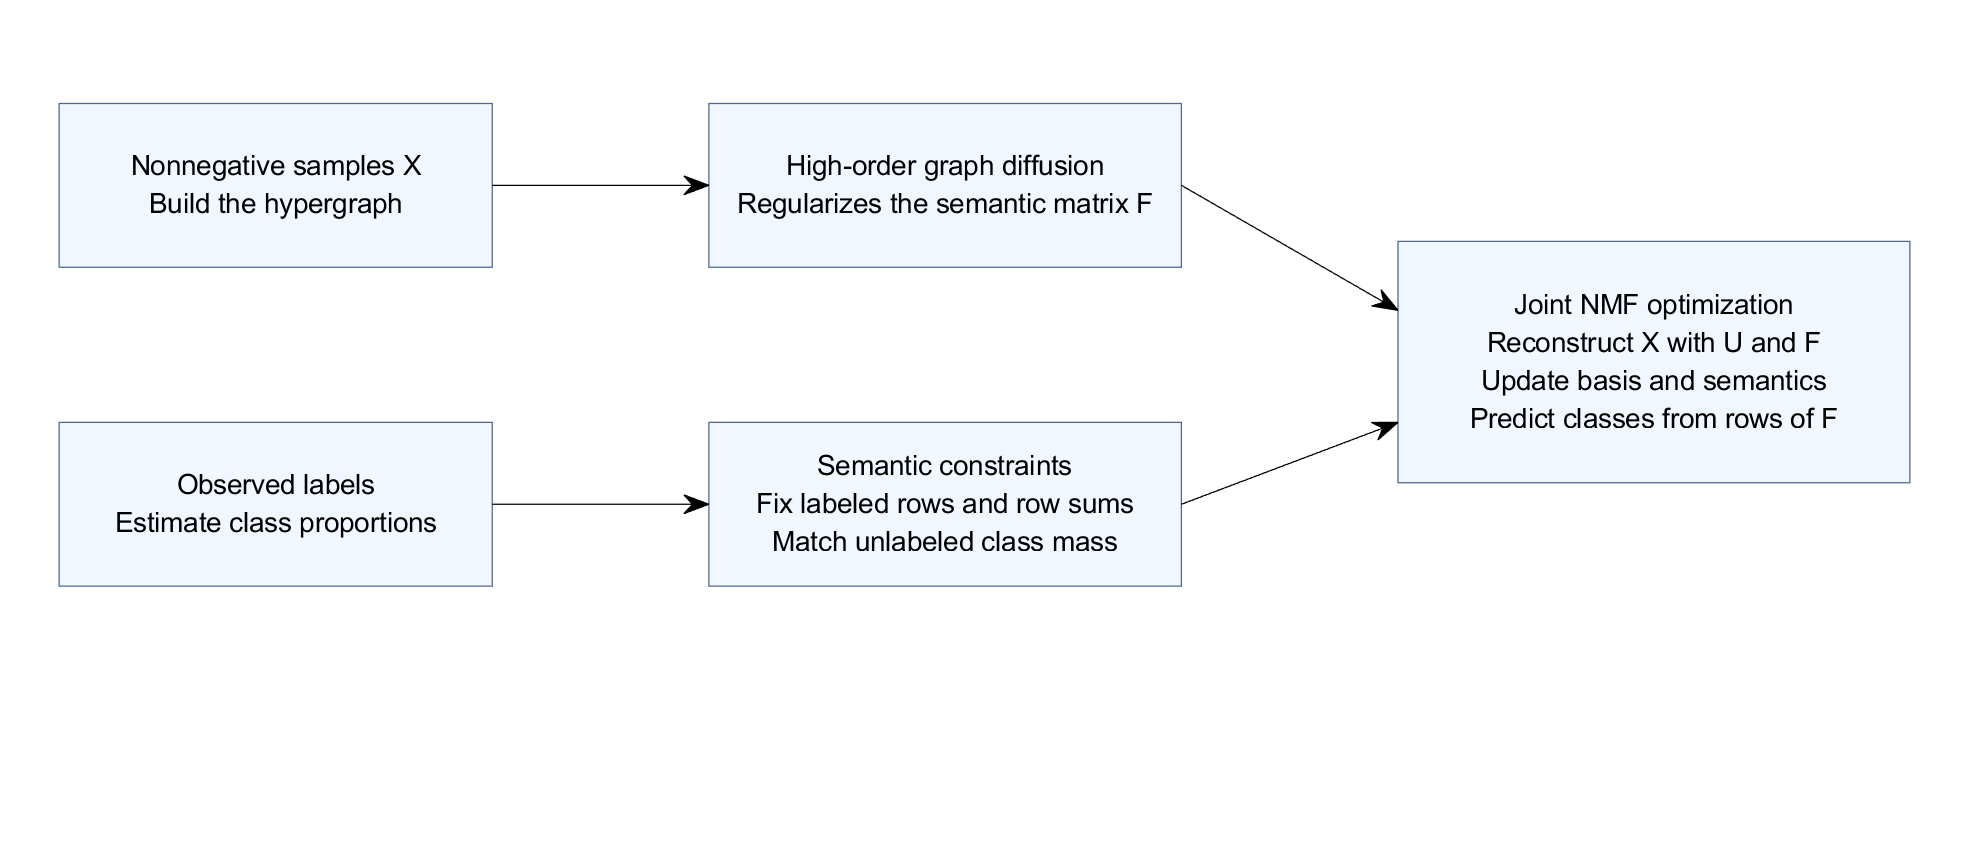
\includegraphics[width=0.96\linewidth]{mechanism.png}
\caption{Mechanism of MCS-NMF. High-order diffusion supplies local structural information, while the transport-polytope constraint preserves the prescribed unlabeled semantic mass across classes.}
\label{fig:mechanism}
\end{figure}

\subsection{Optimization}

For fixed $F$, the multiplicative update of the basis is
\begin{equation}
U\leftarrow U\odotm\frac{XF}{U(F^\top F)+\varepsilon}.
\label{eq:Uupdate}
\end{equation}
The gradient with respect to $F$ is
\begin{equation}
\nabla_F\mathcal J=2\{F(U^\top U)-X^\top U+\alpha L_kF\}.
\label{eq:Fgradient}
\end{equation}
For a trial step $\eta>0$, the unlabeled block is updated in exponentiated form,
\begin{equation}
K=\max(F_U,\varepsilon)\odotm\exp\{-\eta(\nabla_F\mathcal J)_U\}.
\label{eq:mirrortrial}
\end{equation}
Alternating row and column scaling projects $K$ numerically onto $\mathcal T(\pi_L)$:
\begin{equation}
Q\leftarrow\operatorname{diag}\!\left(\frac{\one}{Q\one}\right)Q,
\qquad
Q\leftarrow Q\operatorname{diag}\!\left(\frac{n_U\pi_L}{Q^\top\one}\right).
\label{eq:sinkhorn}
\end{equation}
The trial is accepted when its objective is finite and no larger than the objective before the semantic update; otherwise $\eta$ is halved.

\begin{algorithm}[t]
\caption{MCS-NMF}
\label{alg:mcsnmf}
\begin{minipage}{0.96\linewidth}
\small
\textbf{Input:} $X,Y_L,L_k,\alpha$, maximum cycles $T$, tolerance $\epsilon$.\\
\textbf{Initialize:} $U>0$, $F_U>0$; set $F_L=Y_L$ and scale $F_U$ into $\mathcal T(\pi_L)$.\\
\textbf{for} $t=1,\ldots,T$ \textbf{do}\\
\quad Update $U$ by Eq.~\eqref{eq:Uupdate}.\\
\quad Compute the gradient in Eq.~\eqref{eq:Fgradient}.\\
\quad Form the exponentiated trial in Eq.~\eqref{eq:mirrortrial}.\\
\quad Apply alternating marginal scaling in Eq.~\eqref{eq:sinkhorn}.\\
\quad Accept the trial if the objective does not increase; otherwise halve the step.\\
\quad Restore $F_L=Y_L$ and test the relative objective change.\\
\textbf{end for}\\
\textbf{Output:} $U,F$ and $\hat y_i=\arg\max_j F_{ij}$.
\end{minipage}
\end{algorithm}

\subsection{Computational complexity}

Let $d$, $n$, and $c$ denote the feature, sample, and class counts, let $s=\operatorname{nnz}(L_k)$, and let $R$ and $B$ denote the numbers of marginal-scaling iterations and semantic backtracking trials. One alternating cycle requires
\begin{equation}
\mathcal O\!\left(dnc+nc^2+sc+B(dnc+nc^2+sc+Rnc)\right),
\end{equation}
with memory cost $\mathcal O(dn+dc+nc+s)$. In the present implementation, exact neighbor search used to construct the graph costs $\mathcal O(dn^2)$; the sparse transition representation limits the subsequent diffusion and semantic operations to the observed graph support.

\subsection{Objective-value convergence}

\begin{proposition}
Assume that every accepted semantic trial is finite and belongs to $\mathcal T(\pi_L)$. The alternating cycles of Algorithm~\ref{alg:mcsnmf} preserve nonnegativity and the constraints in Eq.~\eqref{eq:constraints}. Moreover, the sequence $\{\mathcal J(U^{(t)},F^{(t)})\}$ is nonincreasing and converges to a finite limit.
\end{proposition}
\begin{proof}
The multiplicative basis update preserves nonnegativity and is the standard auxiliary-function update for the Frobenius NMF block, hence it does not increase the reconstruction objective for fixed $F$. The semantic trial is positive before marginal scaling. Alternating positive row and column scaling preserves nonnegativity and enforces the two marginals numerically; the labeled block is then restored exactly. Backtracking accepts the semantic block only if the complete objective does not increase. Therefore every accepted cycle is nonincreasing. Both terms in Eq.~\eqref{eq:objective} are nonnegative because $L_k\succeq0$, so the objective sequence is bounded below by zero and consequently converges.
\end{proof}

\begin{remark}
The proposition establishes feasibility preservation and convergence in objective value. The stopping rule uses relative objective change, and the implementation records row and column marginal residuals together with objective monotonicity.
\end{remark}

\section{Experiments}

\subsection{Datasets and evaluation protocol}

We used nine image and handwritten-digit datasets. Table~\ref{tab:datasets} reports their dimensions. All sample vectors were made nonnegative when necessary and normalized to unit Euclidean norm.

\begin{table}[H]
\centering
\caption{Dataset statistics.}
\label{tab:datasets}
\footnotesize
\renewcommand{\arraystretch}{0.90}
\begin{tabular}{lrrr}
\toprule
Dataset & Samples & Features & Classes\\
\midrule
AR & 1680 & 2000 & 120\\
PIE & 2856 & 1024 & 68\\
MSRA25 & 1799 & 256 & 12\\
YaleB & 2414 & 1024 & 38\\
COIL20 & 1440 & 1024 & 20\\
COIL100 & 7200 & 1024 & 100\\
MNIST & 6996 & 784 & 10\\
Palm & 2000 & 256 & 100\\
Optdigits & 5620 & 64 & 10\\
\bottomrule
\end{tabular}
\end{table}

\enlargethispage{4\baselineskip}

For every class containing $n_q$ samples, $\lceil0.1n_q\rceil$ samples were labeled. All methods used the same 20 class-stratified labeled sets, and only unlabeled samples entered evaluation. We compared MCS-NMF with HLPNMF, LpCNMF, PNLPSCONMF, SPNMF, CSDCP, LP, GOCNMF, OCSNMF, SNMFWLP, DSSNMF, ERDNMF, and LSAGNMTF. The six metrics were ACC, NMI, Purity, pair-counting F-score, Precision, and Recall. ACC used evaluation-only optimal assignment \cite{Kuhn1955Hungarian}; NMI followed the geometric-entropy normalization \cite{Vinh2010NMI}.

\begin{landscape}
\subsection{Main comparison}

MCS-NMF ran for at most 100 alternating cycles with a relative-objective tolerance of $10^{-7}$ after 30 cycles. Semantic backtracking allowed 40 halvings, and marginal scaling stopped at its numerical tolerance. Baselines used their native solvers and decision rules under the common data, supervision, and evaluation protocol.

Table~\ref{tab:unified_main} gives the complete six-metric comparison. MCS-NMF achieved the highest mean ACC on eight of nine datasets and the highest mean NMI on eight datasets. ERDNMF obtained the highest AR ACC, and MCS-NMF obtained the highest AR NMI. On Optdigits, the mean NMI difference between MCS-NMF and HLPNMF was $0.008$ percentage points.

\fontsize{6.5}{7.2}\selectfont
\renewcommand{\arraystretch}{0.88}
\setlength{\tabcolsep}{2.2pt}
\begin{longtable}{llrrrrrr}
\caption{Clustering results under the unified paired protocol (mean $\pm$ standard deviation, \%).}\label{tab:unified_main}\\
\toprule Dataset & Method & ACC & NMI & Purity & F-score & Precision & Recall \\
\midrule\endfirsthead
\toprule Dataset & Method & ACC & NMI & Purity & F-score & Precision & Recall \\
\midrule\endhead
AR & MCS-NMF & \underline{76.07 $\pm$ 1.50} & \textbf{88.53 $\pm$ 0.54} & \underline{76.52 $\pm$ 1.45} & \underline{64.01 $\pm$ 1.83} & \textbf{60.07 $\pm$ 2.22} & \underline{68.51 $\pm$ 1.43} \\
 & HLPNMF & 75.11 $\pm$ 1.43 & \underline{88.23 $\pm$ 0.54} & 75.52 $\pm$ 1.42 & 62.21 $\pm$ 1.92 & 57.31 $\pm$ 2.38 & 68.05 $\pm$ 1.41 \\
 & LpCNMF & 75.54 $\pm$ 1.42 & 88.08 $\pm$ 0.53 & 76.05 $\pm$ 1.33 & 62.44 $\pm$ 1.98 & 58.46 $\pm$ 2.38 & 67.02 $\pm$ 1.55 \\
 & PNLPSCONMF & 68.00 $\pm$ 1.65 & 83.06 $\pm$ 0.70 & 68.48 $\pm$ 1.56 & 51.13 $\pm$ 1.94 & 47.35 $\pm$ 2.15 & 55.60 $\pm$ 1.81 \\
 & SPNMF & 40.00 $\pm$ 6.27 & 66.26 $\pm$ 4.34 & 42.25 $\pm$ 6.27 & 7.80 $\pm$ 2.79 & 4.26 $\pm$ 1.66 & 51.60 $\pm$ 6.31 \\
 & CSDCP & 55.44 $\pm$ 1.30 & 83.14 $\pm$ 0.51 & 60.24 $\pm$ 1.02 & 44.16 $\pm$ 1.98 & 36.42 $\pm$ 2.58 & 56.24 $\pm$ 1.20 \\
 & LP & 72.08 $\pm$ 1.36 & 86.89 $\pm$ 0.56 & 72.59 $\pm$ 1.35 & 58.92 $\pm$ 1.86 & 53.62 $\pm$ 2.17 & 65.39 $\pm$ 1.52 \\
 & GOCNMF & 72.01 $\pm$ 1.91 & 86.94 $\pm$ 0.73 & 72.61 $\pm$ 1.78 & 58.32 $\pm$ 2.41 & 53.25 $\pm$ 2.82 & 64.49 $\pm$ 1.91 \\
 & OCSNMF & 71.22 $\pm$ 1.53 & 86.40 $\pm$ 0.48 & 72.09 $\pm$ 1.31 & 57.32 $\pm$ 1.72 & 53.29 $\pm$ 2.00 & 62.03 $\pm$ 1.41 \\
 & SNMFWLP & 57.24 $\pm$ 1.87 & 81.47 $\pm$ 0.98 & 61.23 $\pm$ 1.63 & 33.08 $\pm$ 4.36 & 23.51 $\pm$ 4.39 & 57.01 $\pm$ 1.59 \\
 & DSSNMF & 26.80 $\pm$ 1.53 & 61.74 $\pm$ 1.21 & 28.43 $\pm$ 1.61 & 13.63 $\pm$ 1.42 & 8.77 $\pm$ 1.12 & 31.10 $\pm$ 2.56 \\
 & ERDNMF & \textbf{77.35 $\pm$ 1.91} & 87.86 $\pm$ 0.93 & \textbf{77.60 $\pm$ 1.92} & \textbf{64.06 $\pm$ 2.61} & \underline{59.26 $\pm$ 3.00} & \textbf{69.74 $\pm$ 2.28} \\
 & LSAGNMTF & 60.23 $\pm$ 2.83 & 86.15 $\pm$ 0.98 & 65.61 $\pm$ 2.33 & 47.90 $\pm$ 3.95 & 38.03 $\pm$ 4.50 & 65.14 $\pm$ 1.84 \\
\midrule
PIE & MCS-NMF & \textbf{97.28 $\pm$ 0.51} & \textbf{97.76 $\pm$ 0.33} & \textbf{97.28 $\pm$ 0.51} & \textbf{94.82 $\pm$ 0.87} & \textbf{94.57 $\pm$ 0.96} & \textbf{95.06 $\pm$ 0.79} \\
 & HLPNMF & \underline{96.90 $\pm$ 0.65} & \underline{97.61 $\pm$ 0.35} & \underline{96.90 $\pm$ 0.65} & \underline{94.22 $\pm$ 1.03} & \underline{93.80 $\pm$ 1.22} & \underline{94.65 $\pm$ 0.87} \\
 & LpCNMF & 94.17 $\pm$ 0.57 & 95.14 $\pm$ 0.44 & 94.17 $\pm$ 0.57 & 88.66 $\pm$ 1.17 & 87.92 $\pm$ 1.44 & 89.42 $\pm$ 0.94 \\
 & PNLPSCONMF & 76.54 $\pm$ 2.02 & 82.39 $\pm$ 1.29 & 76.54 $\pm$ 2.02 & 50.91 $\pm$ 4.77 & 42.71 $\pm$ 5.75 & 63.45 $\pm$ 2.38 \\
 & SPNMF & 48.96 $\pm$ 4.71 & 69.56 $\pm$ 4.07 & 52.53 $\pm$ 4.89 & 19.02 $\pm$ 3.76 & 11.87 $\pm$ 2.73 & 49.63 $\pm$ 6.89 \\
 & CSDCP & 73.69 $\pm$ 3.38 & 92.19 $\pm$ 0.94 & 79.01 $\pm$ 2.54 & 72.06 $\pm$ 3.66 & 63.00 $\pm$ 4.72 & 84.33 $\pm$ 2.14 \\
 & LP & 96.15 $\pm$ 0.37 & 96.67 $\pm$ 0.31 & 96.15 $\pm$ 0.37 & 92.62 $\pm$ 0.70 & 92.38 $\pm$ 0.73 & 92.86 $\pm$ 0.67 \\
 & GOCNMF & 95.71 $\pm$ 0.86 & 96.56 $\pm$ 0.55 & 95.71 $\pm$ 0.86 & 91.86 $\pm$ 1.49 & 91.33 $\pm$ 1.66 & 92.40 $\pm$ 1.33 \\
 & OCSNMF & 94.13 $\pm$ 0.70 & 95.30 $\pm$ 0.42 & 94.13 $\pm$ 0.70 & 88.81 $\pm$ 1.16 & 88.02 $\pm$ 1.27 & 89.61 $\pm$ 1.06 \\
 & SNMFWLP & 64.38 $\pm$ 3.15 & 82.05 $\pm$ 2.07 & 69.71 $\pm$ 2.79 & 39.15 $\pm$ 4.82 & 27.73 $\pm$ 4.54 & 67.45 $\pm$ 3.90 \\
 & DSSNMF & 35.42 $\pm$ 1.83 & 65.54 $\pm$ 1.56 & 38.59 $\pm$ 2.00 & 22.64 $\pm$ 2.06 & 16.16 $\pm$ 1.95 & 38.11 $\pm$ 1.86 \\
 & ERDNMF & 78.35 $\pm$ 1.31 & 85.35 $\pm$ 0.75 & 78.63 $\pm$ 1.23 & 66.51 $\pm$ 1.73 & 64.18 $\pm$ 1.71 & 69.02 $\pm$ 1.87 \\
 & LSAGNMTF & 72.78 $\pm$ 2.76 & 90.33 $\pm$ 1.43 & 77.34 $\pm$ 2.54 & 67.27 $\pm$ 4.33 & 58.73 $\pm$ 5.38 & 78.93 $\pm$ 2.83 \\
\midrule
MSRA25 & MCS-NMF & \textbf{99.43 $\pm$ 0.11} & \textbf{98.79 $\pm$ 0.22} & \textbf{99.43 $\pm$ 0.11} & \textbf{98.85 $\pm$ 0.23} & \textbf{98.83 $\pm$ 0.23} & \textbf{98.88 $\pm$ 0.24} \\
 & HLPNMF & \underline{99.39 $\pm$ 0.14} & \underline{98.73 $\pm$ 0.28} & \underline{99.39 $\pm$ 0.14} & \underline{98.76 $\pm$ 0.29} & \underline{98.73 $\pm$ 0.28} & \underline{98.80 $\pm$ 0.31} \\
 & LpCNMF & 98.94 $\pm$ 0.48 & 98.01 $\pm$ 0.71 & 98.94 $\pm$ 0.48 & 97.95 $\pm$ 0.91 & 98.01 $\pm$ 0.82 & 97.89 $\pm$ 1.01 \\
 & PNLPSCONMF & 74.31 $\pm$ 2.79 & 70.56 $\pm$ 2.76 & 74.31 $\pm$ 2.79 & 50.86 $\pm$ 4.99 & 41.30 $\pm$ 5.66 & 66.68 $\pm$ 3.19 \\
 & SPNMF & 86.81 $\pm$ 4.72 & 93.43 $\pm$ 1.82 & 89.09 $\pm$ 3.97 & 85.90 $\pm$ 5.53 & 79.73 $\pm$ 8.63 & 93.63 $\pm$ 2.28 \\
 & CSDCP & 80.03 $\pm$ 7.10 & 88.25 $\pm$ 2.97 & 82.26 $\pm$ 6.24 & 78.30 $\pm$ 6.83 & 70.90 $\pm$ 9.87 & 88.27 $\pm$ 3.39 \\
 & LP & 98.57 $\pm$ 0.89 & 97.66 $\pm$ 0.94 & 98.57 $\pm$ 0.89 & 97.23 $\pm$ 1.54 & 97.02 $\pm$ 1.69 & 97.44 $\pm$ 1.42 \\
 & GOCNMF & 97.66 $\pm$ 0.92 & 96.08 $\pm$ 1.28 & 97.66 $\pm$ 0.92 & 95.52 $\pm$ 1.75 & 95.40 $\pm$ 1.80 & 95.64 $\pm$ 1.73 \\
 & OCSNMF & 96.87 $\pm$ 0.80 & 95.10 $\pm$ 1.01 & 96.87 $\pm$ 0.80 & 94.22 $\pm$ 1.39 & 94.46 $\pm$ 1.31 & 93.98 $\pm$ 1.49 \\
 & SNMFWLP & 85.83 $\pm$ 4.61 & 88.64 $\pm$ 2.78 & 87.15 $\pm$ 3.77 & 82.24 $\pm$ 5.20 & 79.41 $\pm$ 6.69 & 85.40 $\pm$ 3.84 \\
 & DSSNMF & 43.75 $\pm$ 3.18 & 44.47 $\pm$ 2.86 & 45.70 $\pm$ 3.16 & 30.54 $\pm$ 2.89 & 26.50 $\pm$ 3.94 & 36.67 $\pm$ 3.23 \\
 & ERDNMF & 56.90 $\pm$ 2.93 & 49.13 $\pm$ 2.18 & 57.16 $\pm$ 2.69 & 38.71 $\pm$ 2.53 & 36.93 $\pm$ 2.98 & 40.71 $\pm$ 2.21 \\
 & LSAGNMTF & 82.95 $\pm$ 6.00 & 85.38 $\pm$ 3.82 & 84.52 $\pm$ 5.23 & 77.06 $\pm$ 6.86 & 75.14 $\pm$ 8.04 & 79.18 $\pm$ 5.82 \\
\midrule
YaleB & MCS-NMF & \textbf{75.18 $\pm$ 1.09} & \textbf{74.80 $\pm$ 0.72} & \textbf{75.19 $\pm$ 1.08} & \textbf{59.38 $\pm$ 1.23} & \textbf{58.26 $\pm$ 1.36} & \textbf{60.54 $\pm$ 1.15} \\
 & HLPNMF & \underline{74.61 $\pm$ 1.15} & \underline{74.39 $\pm$ 0.81} & \underline{74.61 $\pm$ 1.14} & \underline{58.42 $\pm$ 1.33} & \underline{57.00 $\pm$ 1.46} & \underline{59.92 $\pm$ 1.26} \\
 & LpCNMF & 55.73 $\pm$ 1.78 & 59.32 $\pm$ 1.17 & 55.96 $\pm$ 1.70 & 31.97 $\pm$ 1.48 & 27.58 $\pm$ 1.64 & 38.09 $\pm$ 1.63 \\
 & PNLPSCONMF & 39.21 $\pm$ 1.09 & 40.39 $\pm$ 1.14 & 39.30 $\pm$ 1.05 & 14.78 $\pm$ 1.20 & 11.38 $\pm$ 1.43 & 21.36 $\pm$ 1.08 \\
 & SPNMF & 47.18 $\pm$ 1.48 & 56.55 $\pm$ 1.76 & 48.79 $\pm$ 1.20 & 13.01 $\pm$ 1.42 & 7.71 $\pm$ 1.08 & 43.02 $\pm$ 3.63 \\
 & CSDCP & 40.15 $\pm$ 1.84 & 57.03 $\pm$ 1.24 & 44.22 $\pm$ 1.66 & 25.83 $\pm$ 1.80 & 21.55 $\pm$ 2.11 & 32.37 $\pm$ 1.40 \\
 & LP & 63.40 $\pm$ 1.62 & 65.46 $\pm$ 1.04 & 63.48 $\pm$ 1.60 & 44.67 $\pm$ 2.02 & 42.72 $\pm$ 2.43 & 46.83 $\pm$ 1.69 \\
 & GOCNMF & 72.14 $\pm$ 1.32 & 71.83 $\pm$ 0.85 & 72.15 $\pm$ 1.32 & 54.80 $\pm$ 1.66 & 53.48 $\pm$ 1.95 & 56.19 $\pm$ 1.38 \\
 & OCSNMF & 67.73 $\pm$ 1.08 & 67.21 $\pm$ 0.76 & 67.73 $\pm$ 1.08 & 48.53 $\pm$ 1.38 & 47.51 $\pm$ 1.49 & 49.60 $\pm$ 1.29 \\
 & SNMFWLP & 58.11 $\pm$ 2.12 & 66.02 $\pm$ 1.25 & 59.56 $\pm$ 1.85 & 22.97 $\pm$ 3.30 & 15.10 $\pm$ 2.96 & 49.53 $\pm$ 2.19 \\
 & DSSNMF & 16.35 $\pm$ 0.77 & 30.72 $\pm$ 1.02 & 17.41 $\pm$ 0.76 & 9.64 $\pm$ 0.61 & 7.82 $\pm$ 0.64 & 12.63 $\pm$ 0.71 \\
 & ERDNMF & 22.90 $\pm$ 1.04 & 38.22 $\pm$ 1.06 & 23.92 $\pm$ 1.06 & 14.91 $\pm$ 0.68 & 13.19 $\pm$ 0.85 & 17.18 $\pm$ 0.76 \\
 & LSAGNMTF & 28.44 $\pm$ 1.86 & 42.55 $\pm$ 1.98 & 31.48 $\pm$ 1.36 & 17.60 $\pm$ 1.52 & 14.93 $\pm$ 1.54 & 21.47 $\pm$ 1.49 \\
\midrule
COIL20 & MCS-NMF & \textbf{97.76 $\pm$ 0.65} & \textbf{97.50 $\pm$ 0.63} & \textbf{97.76 $\pm$ 0.65} & \textbf{95.82 $\pm$ 1.16} & \textbf{95.63 $\pm$ 1.24} & \textbf{96.01 $\pm$ 1.08} \\
 & HLPNMF & \underline{95.44 $\pm$ 1.14} & \underline{95.48 $\pm$ 0.99} & \underline{95.44 $\pm$ 1.14} & \underline{91.69 $\pm$ 1.98} & \underline{90.94 $\pm$ 2.28} & \underline{92.46 $\pm$ 1.73} \\
 & LpCNMF & 89.98 $\pm$ 1.30 & 92.37 $\pm$ 0.87 & 90.04 $\pm$ 1.27 & 86.08 $\pm$ 1.33 & 85.33 $\pm$ 1.48 & 86.86 $\pm$ 1.29 \\
 & PNLPSCONMF & 87.59 $\pm$ 2.13 & 88.46 $\pm$ 1.74 & 87.59 $\pm$ 2.13 & 79.84 $\pm$ 3.08 & 77.71 $\pm$ 3.67 & 82.13 $\pm$ 2.62 \\
 & SPNMF & 73.73 $\pm$ 3.95 & 87.67 $\pm$ 2.31 & 77.86 $\pm$ 3.41 & 69.09 $\pm$ 4.44 & 60.49 $\pm$ 5.49 & 80.93 $\pm$ 4.75 \\
 & CSDCP & 79.00 $\pm$ 2.25 & 92.70 $\pm$ 0.70 & 82.82 $\pm$ 1.88 & 79.58 $\pm$ 1.71 & 71.55 $\pm$ 3.63 & 89.89 $\pm$ 2.30 \\
 & LP & 89.04 $\pm$ 0.95 & 92.38 $\pm$ 0.48 & 89.09 $\pm$ 0.92 & 84.90 $\pm$ 0.98 & 81.91 $\pm$ 2.25 & 88.18 $\pm$ 1.42 \\
 & GOCNMF & 92.82 $\pm$ 1.31 & 94.20 $\pm$ 0.76 & 92.82 $\pm$ 1.31 & 88.90 $\pm$ 1.74 & 87.84 $\pm$ 2.34 & 89.99 $\pm$ 1.39 \\
 & OCSNMF & 94.62 $\pm$ 1.06 & 94.55 $\pm$ 0.86 & 94.62 $\pm$ 1.06 & 90.28 $\pm$ 1.87 & 89.55 $\pm$ 2.24 & 91.04 $\pm$ 1.51 \\
 & SNMFWLP & 71.62 $\pm$ 4.10 & 82.36 $\pm$ 3.02 & 74.94 $\pm$ 3.51 & 60.67 $\pm$ 5.64 & 52.69 $\pm$ 6.54 & 71.81 $\pm$ 4.43 \\
 & DSSNMF & 48.20 $\pm$ 3.02 & 62.19 $\pm$ 2.29 & 50.76 $\pm$ 3.02 & 41.09 $\pm$ 3.08 & 36.32 $\pm$ 3.32 & 47.44 $\pm$ 3.18 \\
 & ERDNMF & 70.11 $\pm$ 1.56 & 76.31 $\pm$ 1.59 & 70.40 $\pm$ 1.56 & 62.50 $\pm$ 2.68 & 61.11 $\pm$ 3.05 & 63.97 $\pm$ 2.35 \\
 & LSAGNMTF & 77.13 $\pm$ 4.66 & 88.81 $\pm$ 1.38 & 80.40 $\pm$ 3.49 & 75.98 $\pm$ 3.76 & 70.62 $\pm$ 4.95 & 82.33 $\pm$ 2.45 \\
\midrule
COIL100 & MCS-NMF & \textbf{90.94 $\pm$ 0.38} & \textbf{94.45 $\pm$ 0.21} & \textbf{90.99 $\pm$ 0.38} & \textbf{85.46 $\pm$ 0.65} & \textbf{84.66 $\pm$ 0.76} & \textbf{86.28 $\pm$ 0.60} \\
 & HLPNMF & \underline{89.08 $\pm$ 0.52} & \underline{93.27 $\pm$ 0.31} & \underline{89.09 $\pm$ 0.52} & \underline{82.19 $\pm$ 0.90} & \underline{80.77 $\pm$ 1.10} & 83.66 $\pm$ 0.73 \\
 & LpCNMF & 84.28 $\pm$ 0.41 & 91.02 $\pm$ 0.28 & 84.30 $\pm$ 0.42 & 77.29 $\pm$ 0.66 & 76.11 $\pm$ 0.84 & 78.51 $\pm$ 0.59 \\
 & PNLPSCONMF & 79.18 $\pm$ 0.89 & 86.02 $\pm$ 0.51 & 79.19 $\pm$ 0.89 & 63.98 $\pm$ 1.93 & 59.03 $\pm$ 2.52 & 69.86 $\pm$ 1.13 \\
 & SPNMF & 26.52 $\pm$ 2.02 & 46.31 $\pm$ 2.30 & 28.56 $\pm$ 2.08 & 9.36 $\pm$ 1.23 & 5.98 $\pm$ 0.91 & 21.81 $\pm$ 1.84 \\
 & CSDCP & 68.90 $\pm$ 1.76 & 90.41 $\pm$ 0.41 & 73.29 $\pm$ 1.34 & 66.28 $\pm$ 1.61 & 56.51 $\pm$ 2.22 & 80.22 $\pm$ 1.08 \\
 & LP & 83.02 $\pm$ 0.46 & 90.46 $\pm$ 0.29 & 83.06 $\pm$ 0.47 & 75.52 $\pm$ 0.56 & 73.18 $\pm$ 0.79 & 78.02 $\pm$ 0.56 \\
 & GOCNMF & 86.22 $\pm$ 0.55 & 91.91 $\pm$ 0.32 & 86.23 $\pm$ 0.55 & 79.15 $\pm$ 0.80 & 77.91 $\pm$ 0.95 & 80.42 $\pm$ 0.73 \\
 & OCSNMF & 88.23 $\pm$ 0.53 & 92.63 $\pm$ 0.35 & 88.24 $\pm$ 0.53 & 80.90 $\pm$ 0.94 & 79.71 $\pm$ 1.08 & 82.13 $\pm$ 0.82 \\
 & SNMFWLP & 45.47 $\pm$ 1.33 & 66.80 $\pm$ 1.50 & 50.70 $\pm$ 1.42 & 20.51 $\pm$ 2.28 & 13.68 $\pm$ 1.92 & 41.41 $\pm$ 2.04 \\
 & DSSNMF & 25.81 $\pm$ 0.96 & 55.06 $\pm$ 0.74 & 27.22 $\pm$ 1.08 & 19.31 $\pm$ 0.92 & 13.42 $\pm$ 0.80 & 34.52 $\pm$ 1.61 \\
 & ERDNMF & 55.76 $\pm$ 0.81 & 72.46 $\pm$ 0.60 & 56.02 $\pm$ 0.81 & 43.58 $\pm$ 0.96 & 39.56 $\pm$ 1.13 & 48.54 $\pm$ 0.93 \\
 & LSAGNMTF & 73.27 $\pm$ 1.80 & 92.45 $\pm$ 0.58 & 78.05 $\pm$ 1.49 & 67.93 $\pm$ 2.90 & 56.66 $\pm$ 3.89 & \underline{85.02 $\pm$ 1.43} \\
\midrule
MNIST & MCS-NMF & \textbf{93.78 $\pm$ 0.22} & \textbf{86.14 $\pm$ 0.41} & \textbf{93.78 $\pm$ 0.22} & \textbf{88.28 $\pm$ 0.39} & \textbf{88.15 $\pm$ 0.39} & \textbf{88.40 $\pm$ 0.39} \\
 & HLPNMF & 92.95 $\pm$ 0.28 & 85.09 $\pm$ 0.40 & 92.95 $\pm$ 0.28 & 86.85 $\pm$ 0.47 & 86.62 $\pm$ 0.51 & 87.08 $\pm$ 0.43 \\
 & LpCNMF & 93.08 $\pm$ 0.38 & 85.25 $\pm$ 0.48 & 93.08 $\pm$ 0.38 & 87.07 $\pm$ 0.59 & 86.85 $\pm$ 0.59 & 87.29 $\pm$ 0.60 \\
 & PNLPSCONMF & 77.58 $\pm$ 1.12 & 63.53 $\pm$ 1.21 & 77.58 $\pm$ 1.12 & 61.13 $\pm$ 1.67 & 56.93 $\pm$ 1.98 & 66.00 $\pm$ 1.32 \\
 & SPNMF & 93.09 $\pm$ 0.35 & 84.88 $\pm$ 0.46 & 93.09 $\pm$ 0.35 & 87.00 $\pm$ 0.62 & 86.83 $\pm$ 0.71 & 87.18 $\pm$ 0.55 \\
 & CSDCP & 76.23 $\pm$ 4.01 & 78.15 $\pm$ 0.97 & 76.96 $\pm$ 3.91 & 73.12 $\pm$ 2.72 & 65.37 $\pm$ 4.75 & 83.26 $\pm$ 1.24 \\
 & LP & 92.50 $\pm$ 0.39 & 84.35 $\pm$ 0.45 & 92.50 $\pm$ 0.39 & 86.04 $\pm$ 0.63 & 85.61 $\pm$ 0.69 & 86.48 $\pm$ 0.57 \\
 & GOCNMF & 93.31 $\pm$ 0.25 & 85.33 $\pm$ 0.41 & 93.31 $\pm$ 0.25 & \underline{87.42 $\pm$ 0.43} & \underline{87.25 $\pm$ 0.45} & 87.60 $\pm$ 0.42 \\
 & OCSNMF & 89.50 $\pm$ 0.56 & 78.75 $\pm$ 0.84 & 89.50 $\pm$ 0.56 & 80.80 $\pm$ 0.95 & 80.80 $\pm$ 0.94 & 80.80 $\pm$ 0.97 \\
 & SNMFWLP & \underline{93.31 $\pm$ 0.28} & \underline{85.47 $\pm$ 0.45} & \underline{93.31 $\pm$ 0.28} & 87.42 $\pm$ 0.50 & 87.24 $\pm$ 0.53 & \underline{87.60 $\pm$ 0.47} \\
 & DSSNMF & 42.00 $\pm$ 3.03 & 36.71 $\pm$ 2.02 & 46.21 $\pm$ 2.37 & 31.06 $\pm$ 1.97 & 28.84 $\pm$ 2.25 & 33.72 $\pm$ 2.04 \\
 & ERDNMF & 56.60 $\pm$ 1.70 & 45.92 $\pm$ 1.45 & 58.39 $\pm$ 1.53 & 41.82 $\pm$ 1.35 & 41.48 $\pm$ 1.34 & 42.16 $\pm$ 1.36 \\
 & LSAGNMTF & 83.43 $\pm$ 5.49 & 78.04 $\pm$ 1.69 & 85.35 $\pm$ 3.45 & 76.45 $\pm$ 3.79 & 74.56 $\pm$ 5.37 & 78.54 $\pm$ 2.42 \\
\midrule
Palm & MCS-NMF & \textbf{95.59 $\pm$ 0.86} & \textbf{98.05 $\pm$ 0.31} & \textbf{95.62 $\pm$ 0.85} & \textbf{92.98 $\pm$ 1.17} & \textbf{91.42 $\pm$ 1.54} & \textbf{94.60 $\pm$ 0.83} \\
 & HLPNMF & 95.10 $\pm$ 0.91 & \underline{97.89 $\pm$ 0.33} & 95.12 $\pm$ 0.90 & \underline{92.23 $\pm$ 1.27} & \underline{90.43 $\pm$ 1.63} & \underline{94.11 $\pm$ 0.91} \\
 & LpCNMF & 92.36 $\pm$ 1.65 & 97.24 $\pm$ 0.54 & 92.61 $\pm$ 1.53 & 88.28 $\pm$ 2.26 & 84.66 $\pm$ 2.91 & 92.23 $\pm$ 1.59 \\
 & PNLPSCONMF & 81.92 $\pm$ 2.31 & 89.96 $\pm$ 1.11 & 81.96 $\pm$ 2.28 & 65.57 $\pm$ 4.17 & 57.68 $\pm$ 5.23 & 76.14 $\pm$ 2.41 \\
 & SPNMF & 42.62 $\pm$ 3.34 & 72.90 $\pm$ 2.41 & 45.58 $\pm$ 3.42 & 27.69 $\pm$ 3.74 & 19.32 $\pm$ 3.24 & 49.49 $\pm$ 4.04 \\
 & CSDCP & 68.38 $\pm$ 2.88 & 92.14 $\pm$ 0.76 & 74.77 $\pm$ 2.17 & 65.50 $\pm$ 3.20 & 54.64 $\pm$ 3.89 & 81.92 $\pm$ 1.73 \\
 & LP & 91.94 $\pm$ 1.39 & 96.39 $\pm$ 0.70 & 92.02 $\pm$ 1.36 & 74.55 $\pm$ 6.60 & 63.08 $\pm$ 8.77 & 91.93 $\pm$ 1.28 \\
 & GOCNMF & 86.78 $\pm$ 1.97 & 95.24 $\pm$ 0.61 & 87.23 $\pm$ 1.82 & 81.32 $\pm$ 2.32 & 76.88 $\pm$ 2.87 & 86.33 $\pm$ 1.71 \\
 & OCSNMF & 87.25 $\pm$ 1.83 & 94.18 $\pm$ 1.06 & 87.48 $\pm$ 1.83 & 65.06 $\pm$ 9.89 & 52.94 $\pm$ 11.67 & 86.69 $\pm$ 1.62 \\
 & SNMFWLP & 56.60 $\pm$ 2.41 & 82.45 $\pm$ 1.71 & 63.22 $\pm$ 2.13 & 24.42 $\pm$ 6.72 & 15.17 $\pm$ 5.26 & 68.27 $\pm$ 3.14 \\
 & DSSNMF & 36.85 $\pm$ 1.72 & 67.45 $\pm$ 1.16 & 38.70 $\pm$ 1.83 & 23.74 $\pm$ 1.82 & 17.10 $\pm$ 1.71 & 39.05 $\pm$ 2.08 \\
 & ERDNMF & \underline{95.16 $\pm$ 0.97} & 97.10 $\pm$ 0.49 & \underline{95.16 $\pm$ 0.97} & 91.56 $\pm$ 1.43 & 90.36 $\pm$ 1.83 & 92.80 $\pm$ 1.09 \\
 & LSAGNMTF & 67.71 $\pm$ 2.33 & 91.27 $\pm$ 0.74 & 73.58 $\pm$ 1.82 & 62.40 $\pm$ 3.07 & 51.30 $\pm$ 3.67 & 79.83 $\pm$ 2.23 \\
\midrule
Optdigits & MCS-NMF & \textbf{98.55 $\pm$ 0.09} & \underline{96.23 $\pm$ 0.20} & \textbf{98.55 $\pm$ 0.09} & \textbf{97.12 $\pm$ 0.17} & \textbf{97.11 $\pm$ 0.17} & \textbf{97.14 $\pm$ 0.17} \\
 & HLPNMF & \underline{98.54 $\pm$ 0.12} & \textbf{96.24 $\pm$ 0.22} & \underline{98.54 $\pm$ 0.12} & \underline{97.11 $\pm$ 0.23} & \underline{97.11 $\pm$ 0.23} & \underline{97.12 $\pm$ 0.23} \\
 & LpCNMF & 98.40 $\pm$ 0.10 & 95.91 $\pm$ 0.22 & 98.40 $\pm$ 0.10 & 96.83 $\pm$ 0.20 & 96.81 $\pm$ 0.20 & 96.85 $\pm$ 0.20 \\
 & PNLPSCONMF & 92.55 $\pm$ 0.97 & 84.99 $\pm$ 1.29 & 92.55 $\pm$ 0.97 & 85.99 $\pm$ 1.71 & 85.41 $\pm$ 1.97 & 86.59 $\pm$ 1.44 \\
 & SPNMF & 90.11 $\pm$ 4.24 & 93.15 $\pm$ 1.44 & 90.66 $\pm$ 3.92 & 89.41 $\pm$ 3.74 & 83.96 $\pm$ 6.50 & 95.86 $\pm$ 0.96 \\
 & CSDCP & 92.32 $\pm$ 4.87 & 93.95 $\pm$ 1.36 & 92.59 $\pm$ 4.64 & 91.29 $\pm$ 4.21 & 87.12 $\pm$ 7.69 & 96.24 $\pm$ 0.33 \\
 & LP & 98.41 $\pm$ 0.13 & 95.95 $\pm$ 0.26 & 98.41 $\pm$ 0.13 & 96.85 $\pm$ 0.25 & 96.83 $\pm$ 0.25 & 96.87 $\pm$ 0.24 \\
 & GOCNMF & 98.27 $\pm$ 0.22 & 95.72 $\pm$ 0.45 & 98.27 $\pm$ 0.22 & 96.58 $\pm$ 0.42 & 96.55 $\pm$ 0.43 & 96.60 $\pm$ 0.41 \\
 & OCSNMF & 97.29 $\pm$ 0.29 & 93.62 $\pm$ 0.57 & 97.29 $\pm$ 0.29 & 94.70 $\pm$ 0.54 & 94.68 $\pm$ 0.55 & 94.72 $\pm$ 0.53 \\
 & SNMFWLP & 95.35 $\pm$ 5.21 & 94.85 $\pm$ 1.62 & 95.85 $\pm$ 4.27 & 94.07 $\pm$ 4.43 & 92.42 $\pm$ 7.32 & 96.03 $\pm$ 1.25 \\
 & DSSNMF & 55.40 $\pm$ 6.95 & 50.38 $\pm$ 5.66 & 57.83 $\pm$ 6.50 & 43.99 $\pm$ 5.98 & 41.41 $\pm$ 6.59 & 47.03 $\pm$ 5.33 \\
 & ERDNMF & 82.28 $\pm$ 0.66 & 71.07 $\pm$ 0.66 & 82.28 $\pm$ 0.66 & 70.13 $\pm$ 0.77 & 69.71 $\pm$ 0.86 & 70.56 $\pm$ 0.70 \\
 & LSAGNMTF & 96.10 $\pm$ 2.67 & 92.60 $\pm$ 1.31 & 96.25 $\pm$ 2.00 & 93.10 $\pm$ 2.35 & 92.79 $\pm$ 3.41 & 93.45 $\pm$ 1.32 \\
\bottomrule
\end{longtable}
\end{landscape}


Figure~\ref{fig:heatmap} summarizes ACC and NMI across the full comparison. It is used as a visual overview; exact values remain in Table~\ref{tab:unified_main}.

\begin{figure}[!htbp]
\centering
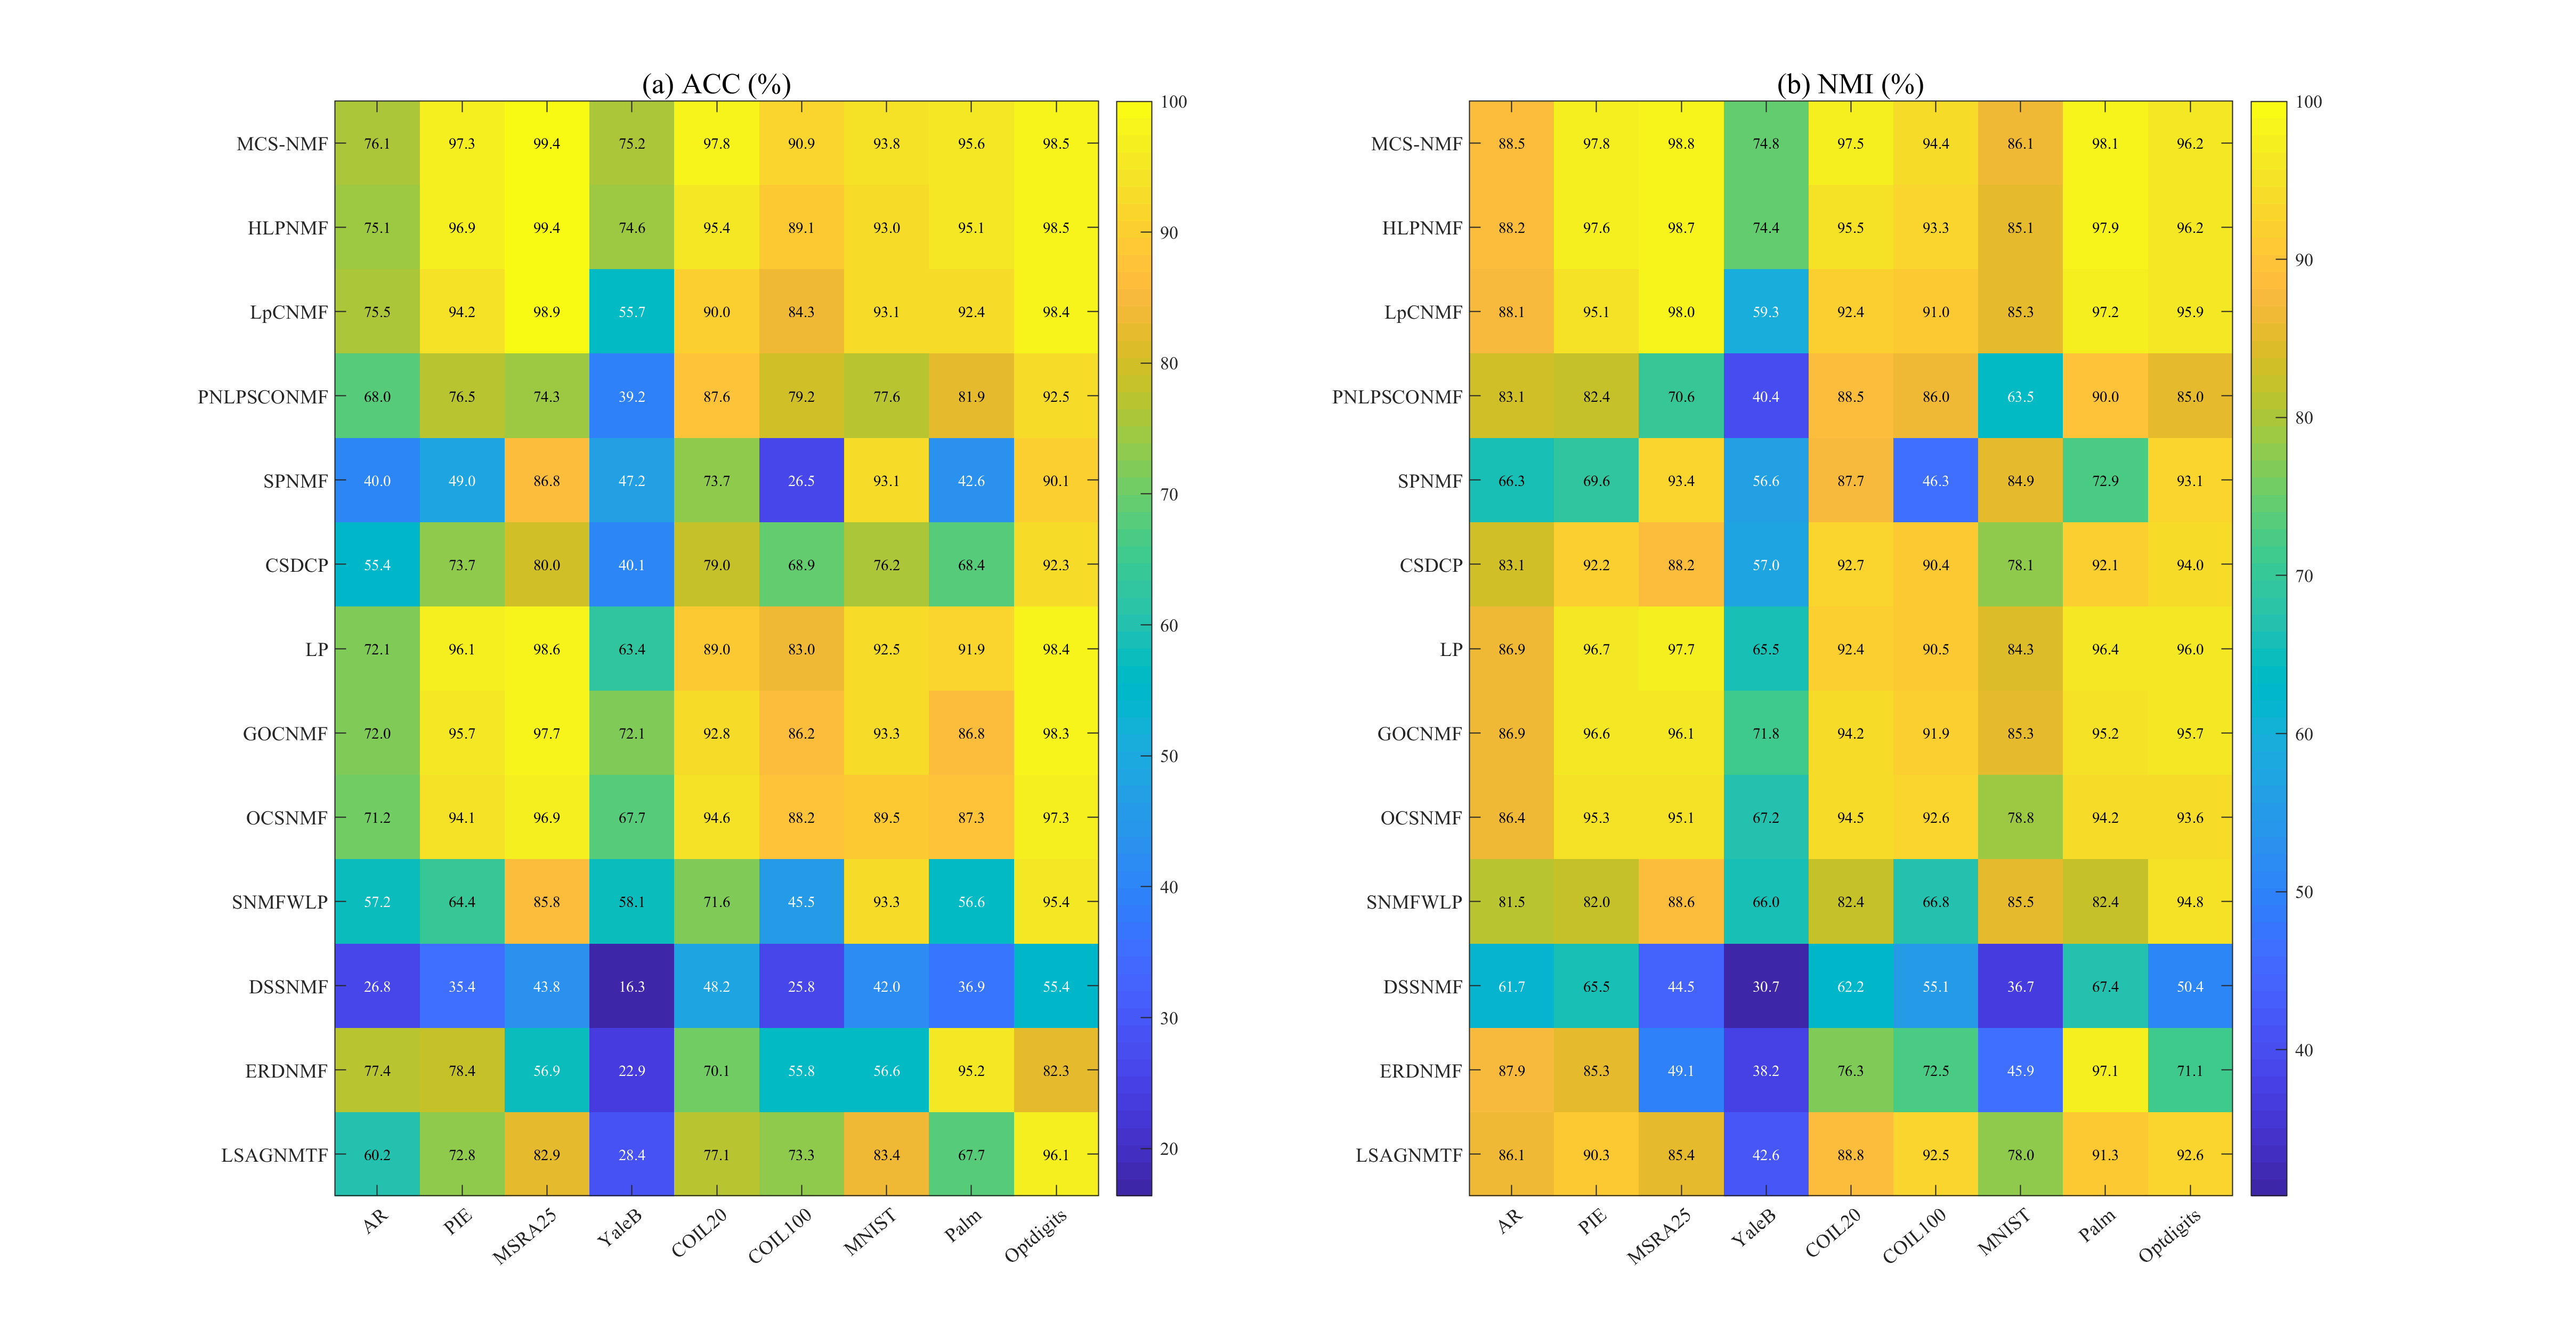
\includegraphics[width=0.96\textwidth]{main_heatmap.png}
\caption{Mean ACC and NMI for MCS-NMF and 12 baselines on nine datasets under the shared paired protocol.}
\label{fig:heatmap}
\end{figure}

\subsection{Paired statistical analysis}

For each baseline, dataset, and metric, we formed the within-mask difference between MCS-NMF and the baseline. We used two-sided paired $t$-tests, 10,000 paired bootstrap resamples, and Holm adjustment within each metric family. The analysis contains 648 comparisons. MCS-NMF had a positive mean difference in 107 of 108 comparisons for ACC, NMI, Purity, F-score, and Recall, and in all 108 Precision comparisons. The bootstrap interval lay entirely above zero in 104 ACC, 106 NMI, 104 Purity, and 105 F-score, Precision, and Recall comparisons.

The main exception was AR versus ERDNMF: the ACC difference was $-1.281$ percentage points with a 95\% bootstrap interval of $[-2.170,-0.410]$. On Optdigits, the NMI difference relative to HLPNMF was $-0.008$ points with an interval of $[-0.099,0.085]$. Figure~\ref{fig:paired} shows the paired ACC and NMI effects against the prespecified comparator HLPNMF.

\begin{figure}[!htbp]
\centering
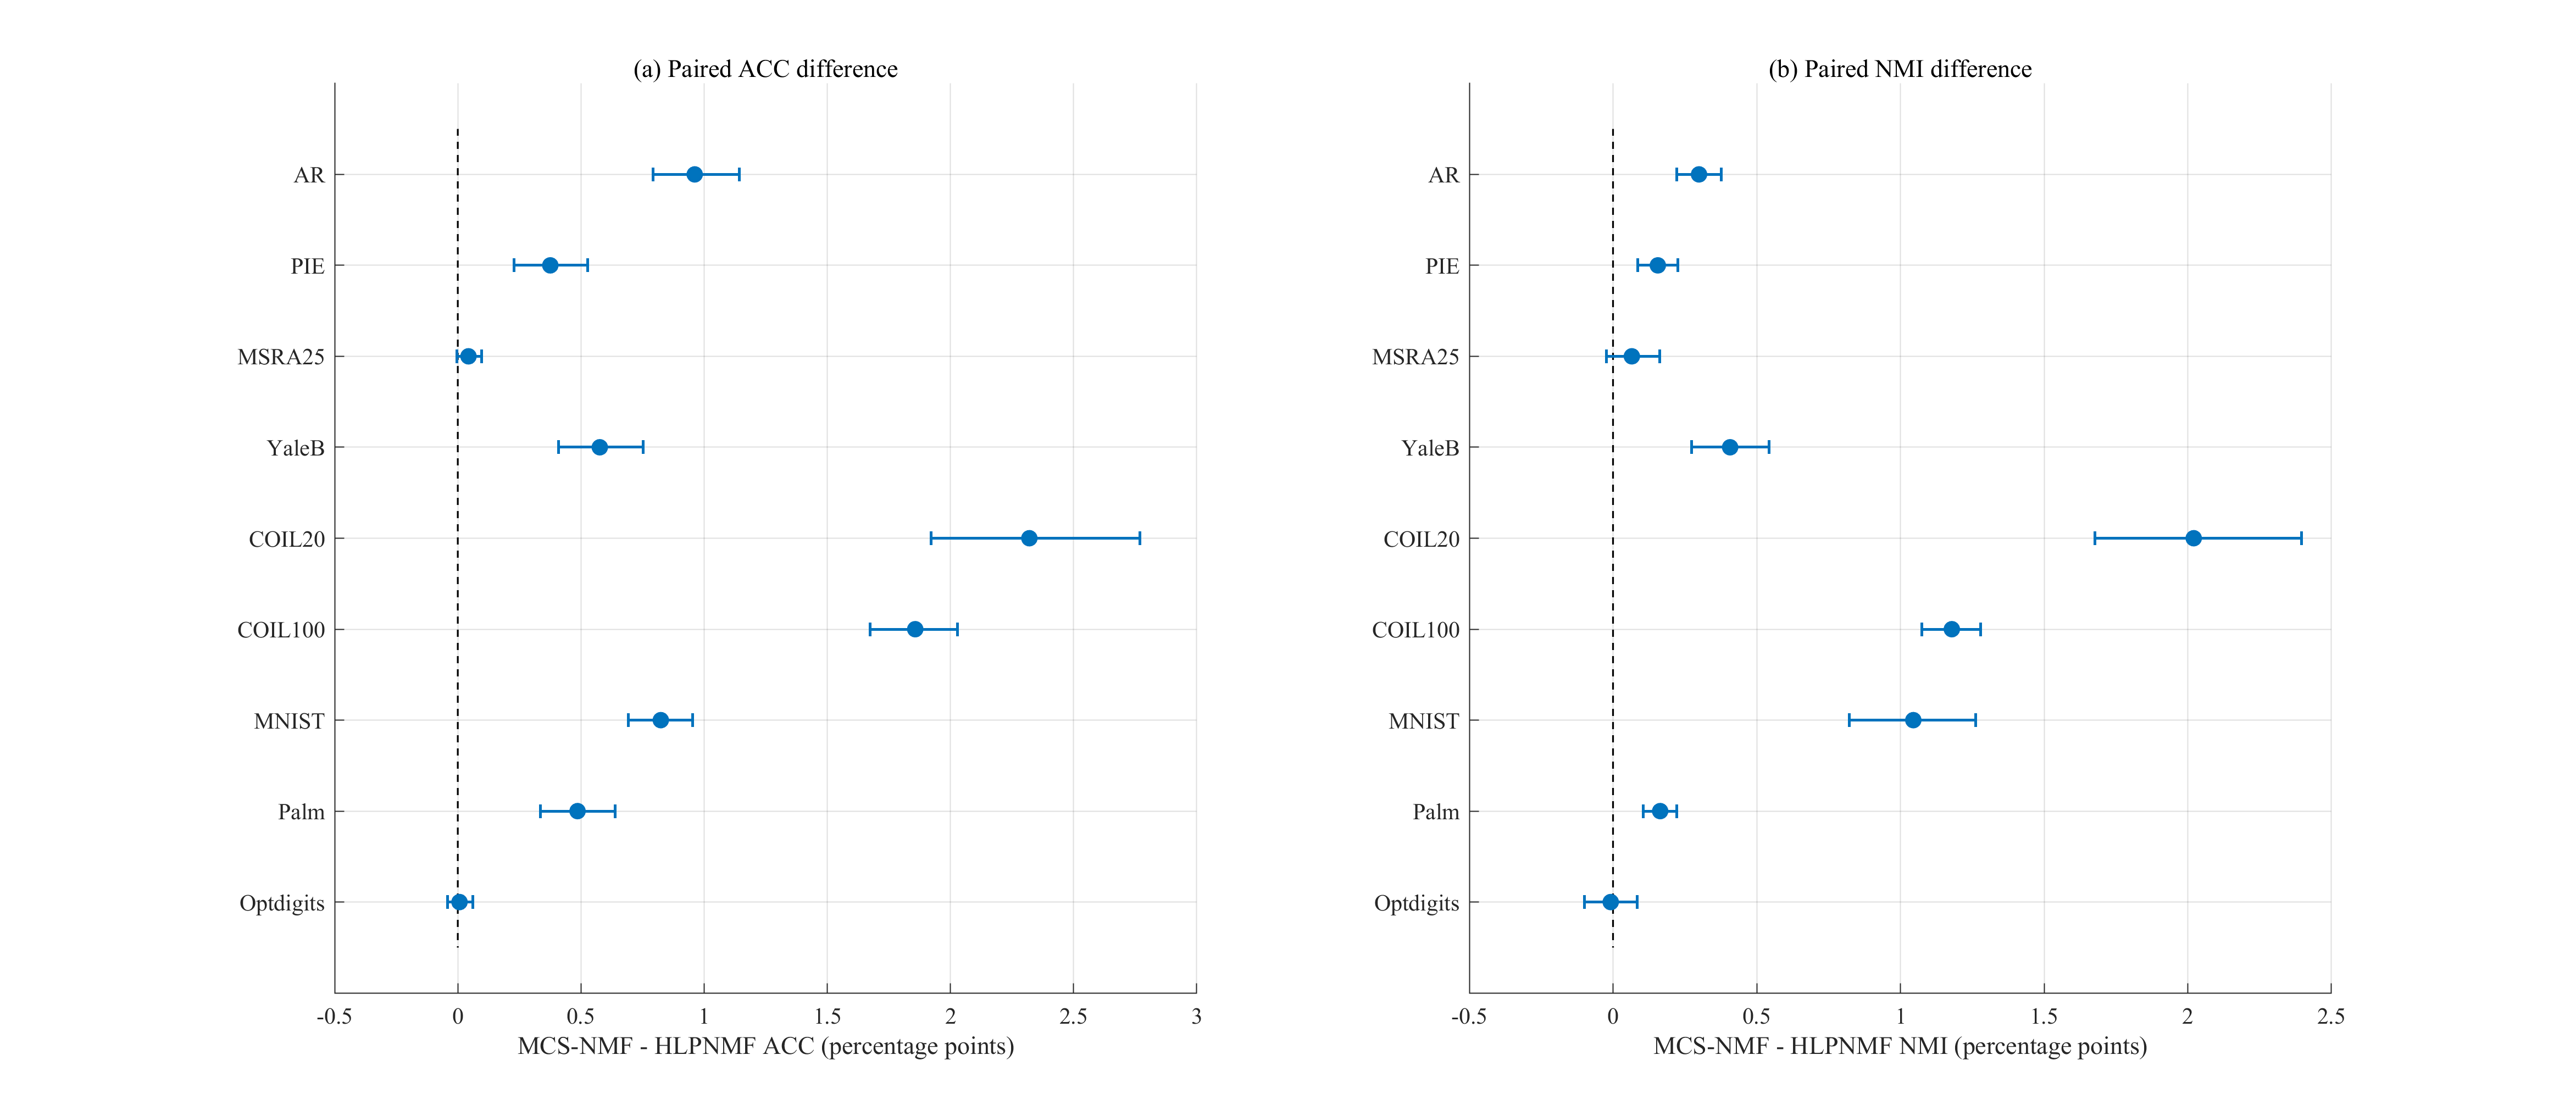
\includegraphics[width=0.94\textwidth]{paired_differences.png}
\caption{Paired ACC and NMI differences between MCS-NMF and HLPNMF. Points are mean paired differences; bars are 95\% percentile-bootstrap intervals from 10,000 paired resamples.}
\label{fig:paired}
\end{figure}

Table~\ref{tab:paired_significance} condenses the Holm-adjusted ACC and NMI tests and reports the distinct outcomes on AR and Optdigits.

\begin{table}[H]
\centering
\caption{Paired significance of MCS-NMF against the competing methods. Symbols $+$, $-$, and 0 denote significantly better, significantly worse, or no significant difference after Holm adjustment, respectively (two-sided paired $t$-tests, familywise $\alpha=0.05$).}
\label{tab:paired_significance}
\setlength{\tabcolsep}{3.2pt}
\small
\renewcommand{\arraystretch}{0.78}
\resizebox{\textwidth}{!}{%
\begin{tabular}{llccccccccc}
\toprule
Metric & Baseline & AR & PIE & MSRA25 & YaleB & COIL20 & COIL100 & MNIST & Palm & Optdigits \\
\midrule
\multirow{12}{*}{ACC} & HLPNMF & + & + & 0 & + & + & + & + & + & 0 \\
 & LpCNMF & + & + & + & + & + & + & + & + & + \\
 & PNLPSCONMF & + & + & + & + & + & + & + & + & + \\
 & SPNMF & + & + & + & + & + & + & + & + & + \\
 & CSDCP & + & + & + & + & + & + & + & + & + \\
 & LP & + & + & + & + & + & + & + & + & + \\
 & GOCNMF & + & + & + & + & + & + & + & + & + \\
 & OCSNMF & + & + & + & + & + & + & + & + & + \\
 & SNMFWLP & + & + & + & + & + & + & + & + & 0 \\
 & DSSNMF & + & + & + & + & + & + & + & + & + \\
 & ERDNMF & 0 & + & + & + & + & + & + & 0 & + \\
 & LSAGNMTF & + & + & + & + & + & + & + & + & + \\
\midrule
\multirow{12}{*}{NMI} & HLPNMF & + & + & 0 & + & + & + & + & + & 0 \\
 & LpCNMF & + & + & + & + & + & + & + & + & + \\
 & PNLPSCONMF & + & + & + & + & + & + & + & + & + \\
 & SPNMF & + & + & + & + & + & + & + & + & + \\
 & CSDCP & + & + & + & + & + & + & + & + & + \\
 & LP & + & + & + & + & + & + & + & + & + \\
 & GOCNMF & + & + & + & + & + & + & + & + & + \\
 & OCSNMF & + & + & + & + & + & + & + & + & + \\
 & SNMFWLP & + & + & + & + & + & + & + & + & + \\
 & DSSNMF & + & + & + & + & + & + & + & + & + \\
 & ERDNMF & + & + & + & + & + & + & + & + & + \\
 & LSAGNMTF & + & + & + & + & + & + & + & + & + \\
\bottomrule
\end{tabular}}
\end{table}


\subsection{Influence of supervision}

We varied the requested supervision ratio over $\{5\%,10\%,15\%,20\%,30\%\}$ on PIE, MSRA25, COIL20, and MNIST using paired labeled sets within each budget. Figure~\ref{fig:supervision} shows that increasing supervision generally improves ACC and NMI, with the largest gains occurring at the lower budgets. The comparison also shows the effect of mass conservation under limited labels.

\begin{figure}[!htbp]
\centering
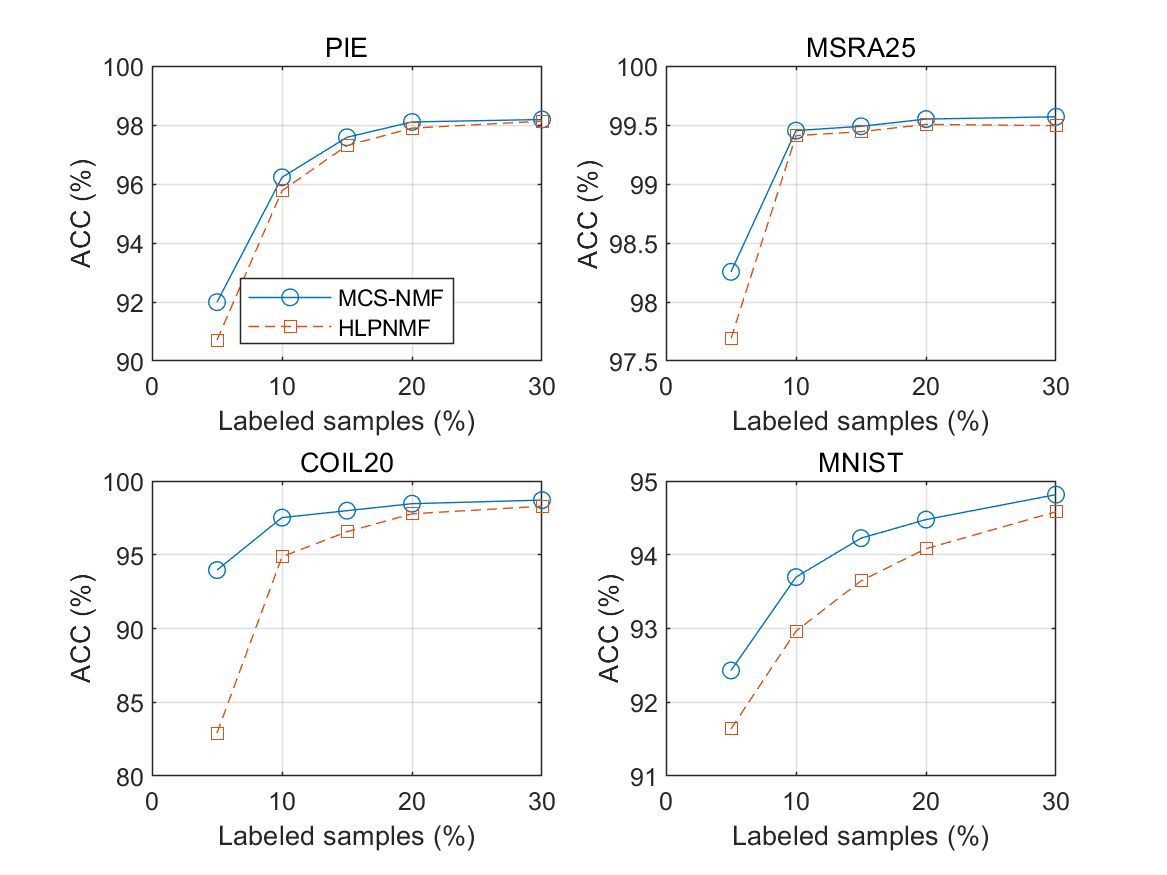
\includegraphics[width=0.48\textwidth]{supervision_acc.png}\hfill
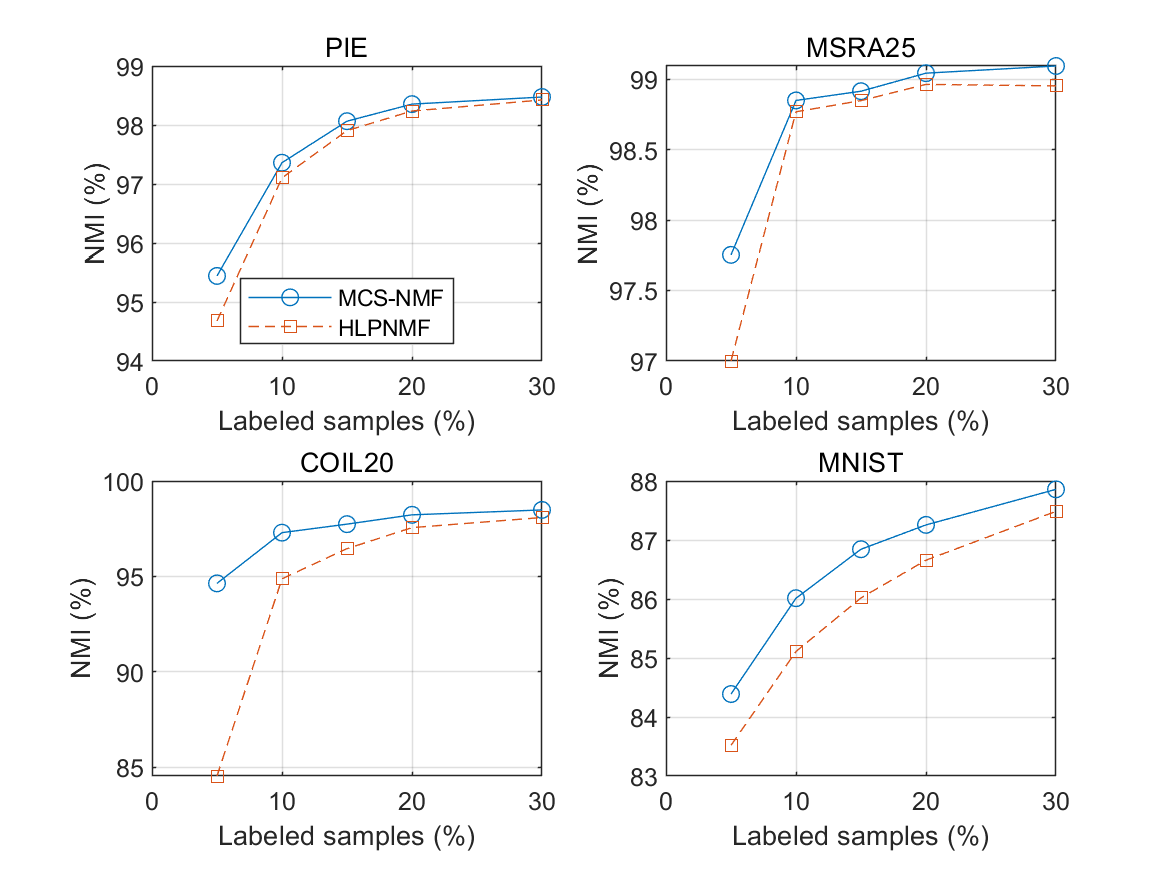
\includegraphics[width=0.48\textwidth]{supervision_nmi.png}
\caption{Influence of the supervision ratio on ACC and NMI.}
\label{fig:supervision}
\end{figure}

\subsection{Parameter sensitivity}

We varied the diffusion weight $\alpha\in\{10^{-3},10^{-2},10^{-1},1,10,10^2,10^3\}$, neighborhood size $p\in\{2,3,5,7,10\}$, propagation order $k\in\{1,\ldots,6\}$, and iteration limit $T\in\{10,15,20,25,30,35,40\}$. Figure~\ref{fig:parameters} reports ACC and NMI on eight datasets. Performance improves sharply as $\alpha$ moves from an under-regularized range and then stabilizes on most datasets. The preferred neighborhood size is data dependent, while the curves over $k$ and $T$ are comparatively stable after their initial region.

\begin{figure}[!htbp]
\centering
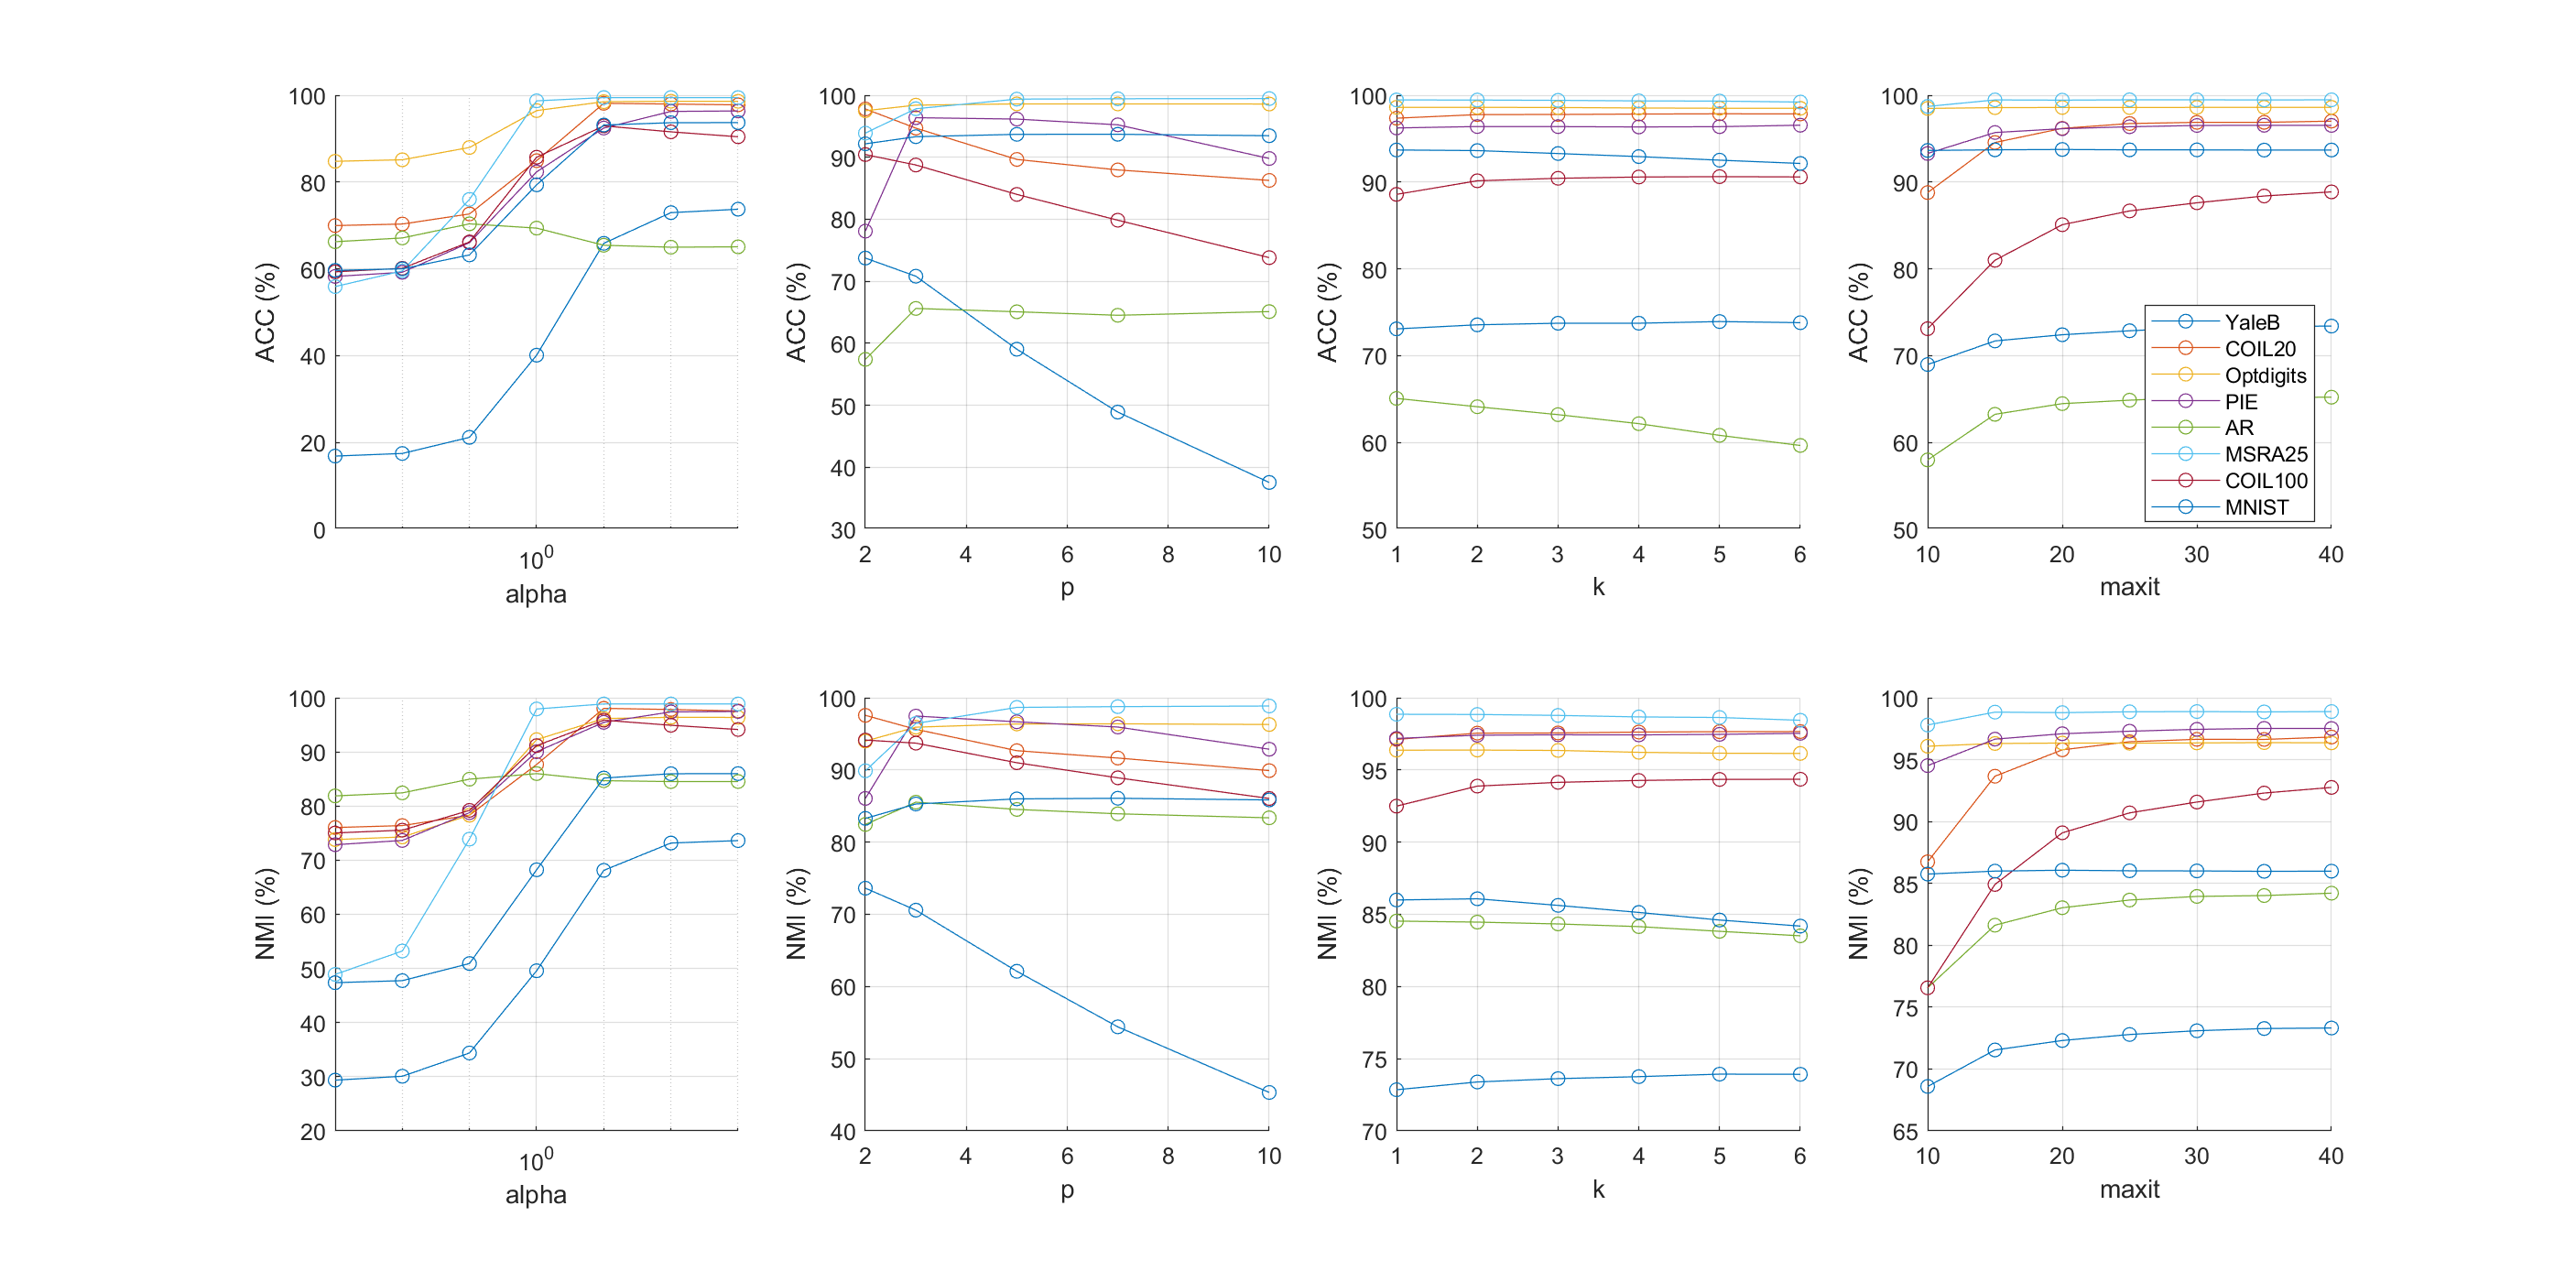
\includegraphics[width=0.99\textwidth]{parameter_sensitivity_full.png}
\caption{ACC and NMI sensitivity to $\alpha$, neighborhood size $p$, propagation order $k$, and iteration limit $T$.}
\label{fig:parameters}
\end{figure}

\subsection{Robustness and ablation}

We corrupted $10\%$--$50\%$ of the samples in COIL20, YaleB, and PIE using either salt-and-pepper noise of density 0.1 or a random $5\times5$ black block. Each condition used five paired runs. Figure~\ref{fig:noiseexamples} illustrates both corruptions. Figures~\ref{fig:noiserobustness} and \ref{fig:robustness} show that MCS-NMF retains higher ACC and NMI than HLPNMF throughout the salt-and-pepper tests. The block-occlusion curves record the strongest separation at severe corruption on YaleB and PIE.

\begin{figure}[!htbp]
\centering
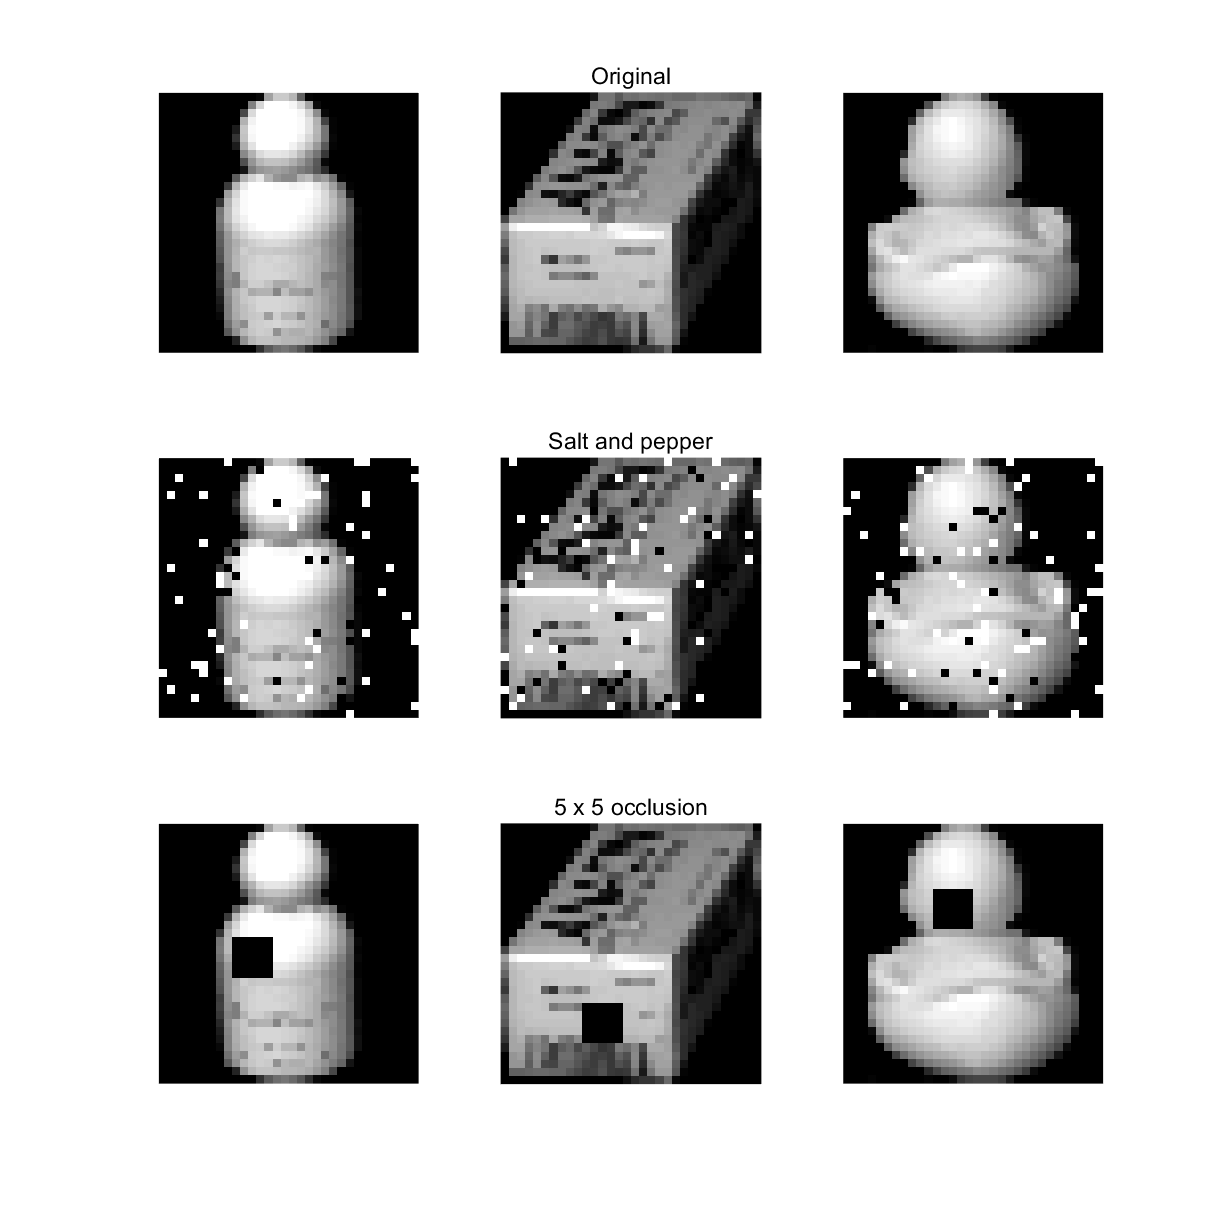
\includegraphics[width=0.78\textwidth]{noise_examples.png}
\caption{Examples of original COIL20 images, salt-and-pepper corruption, and $5\times5$ block occlusion.}
\label{fig:noiseexamples}
\end{figure}

\begin{figure}[!htbp]
\centering
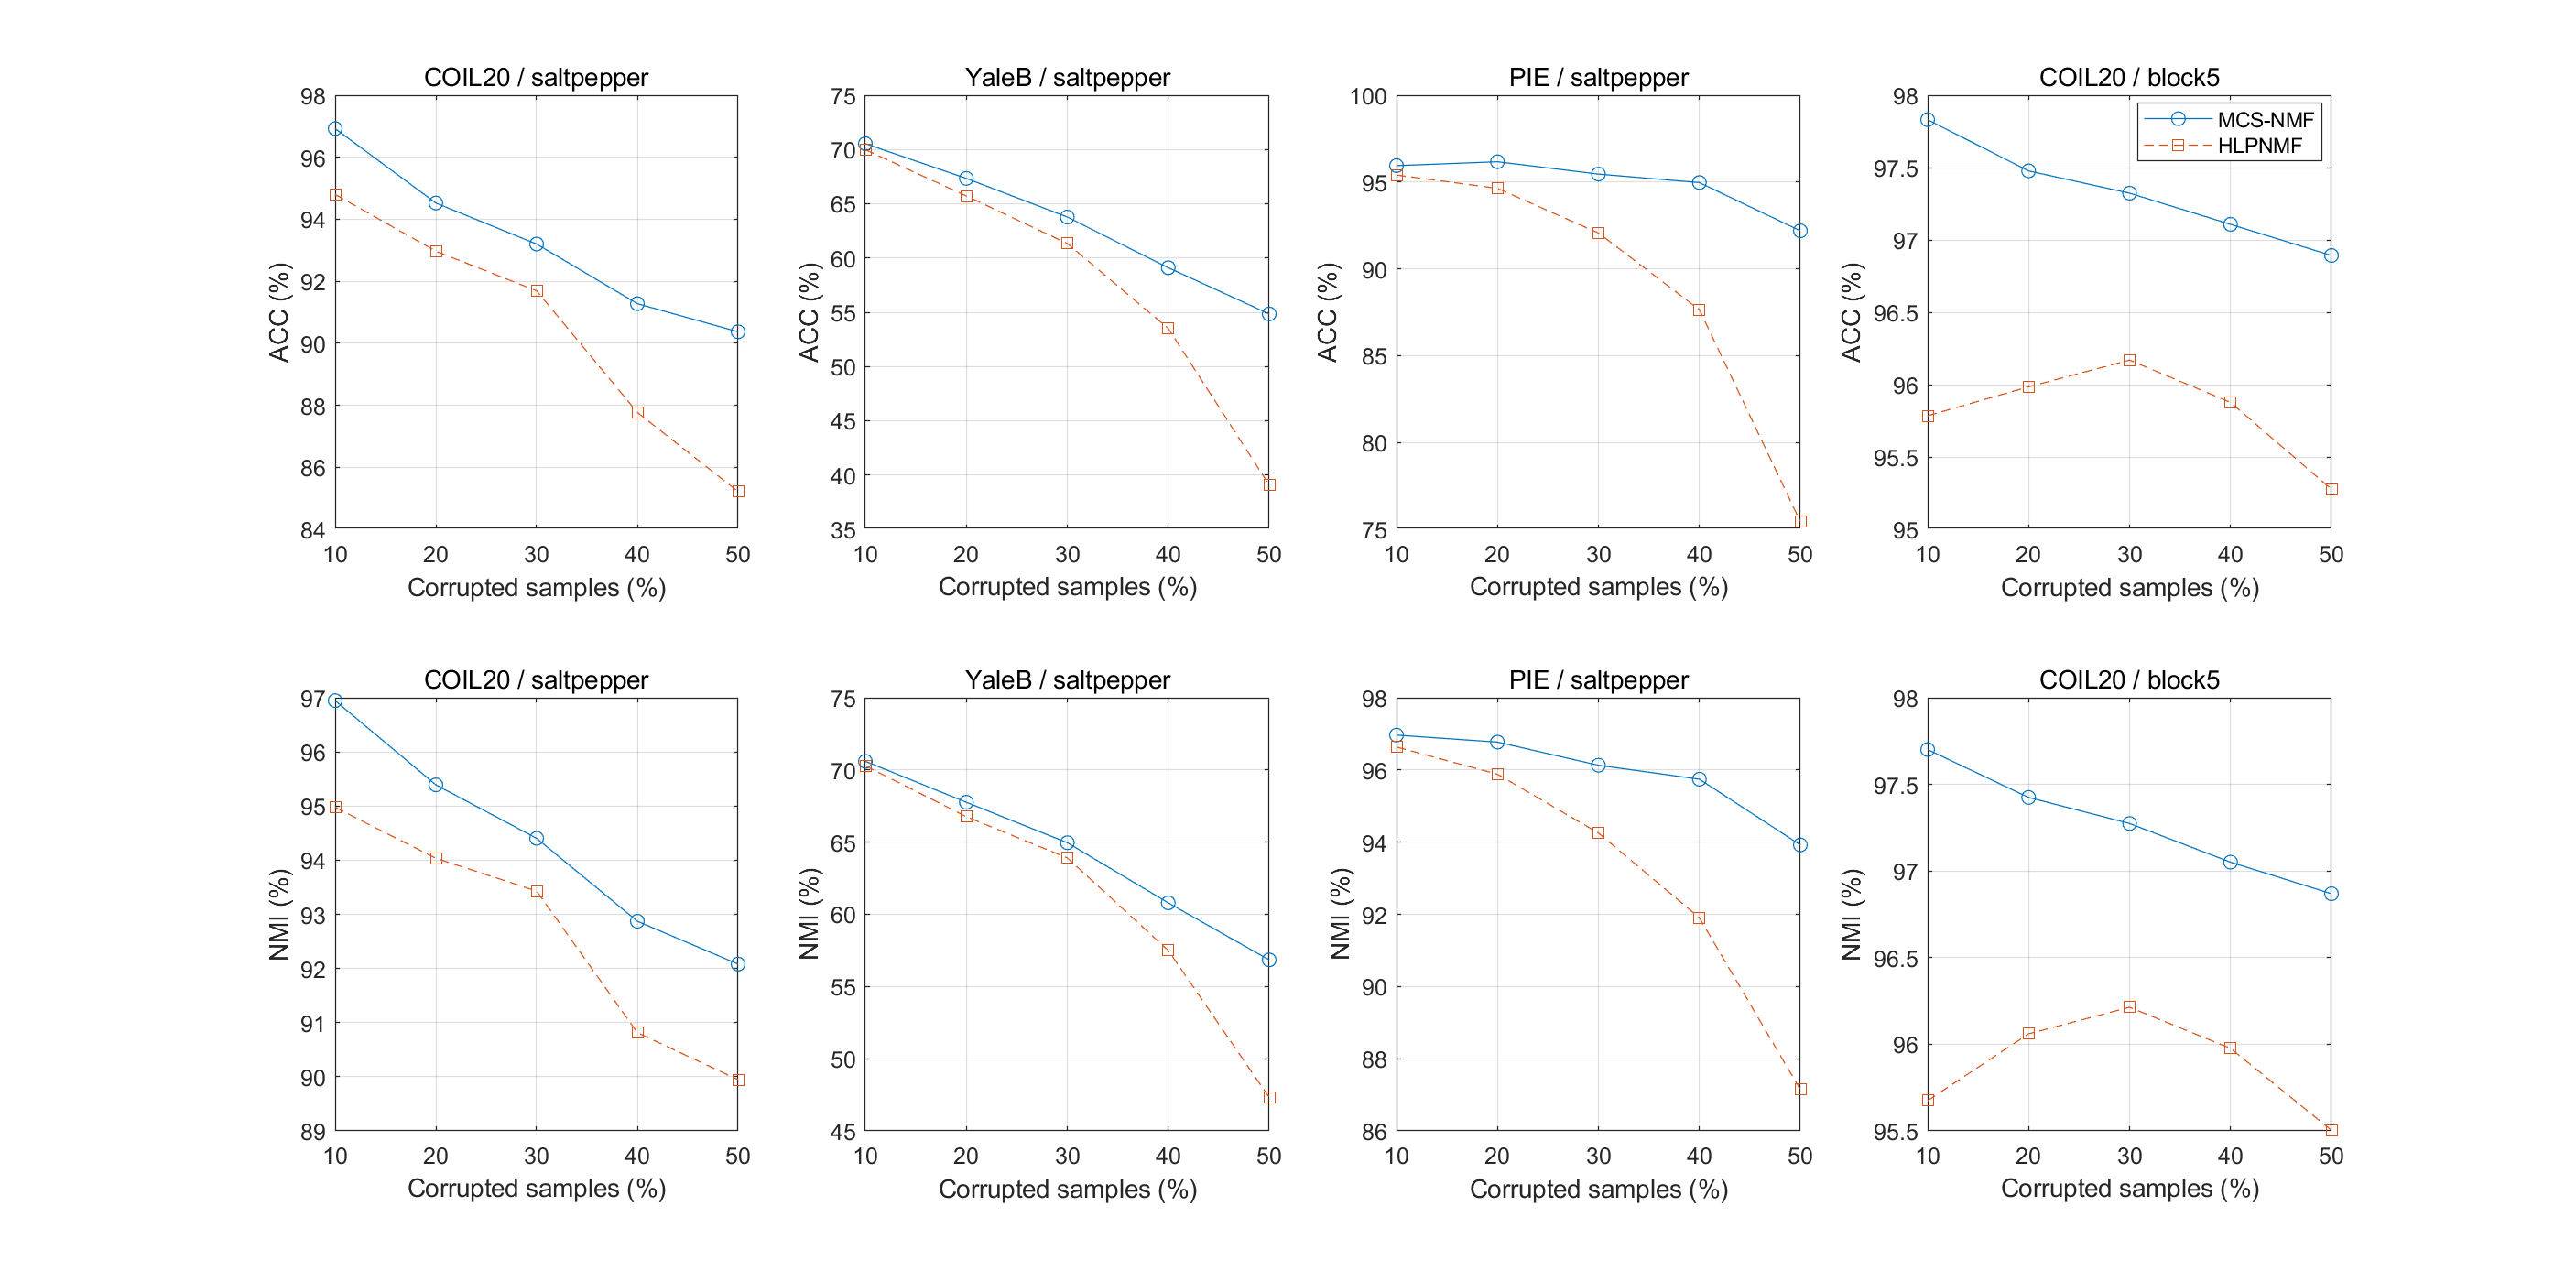
\includegraphics[width=0.99\textwidth]{noise_robustness_full.png}
\caption{ACC and NMI of MCS-NMF and HLPNMF under salt-and-pepper noise on COIL20, YaleB, and PIE, together with the representative COIL20 block-occlusion result.}
\label{fig:noiserobustness}
\end{figure}

\begin{figure}[!htbp]
\centering
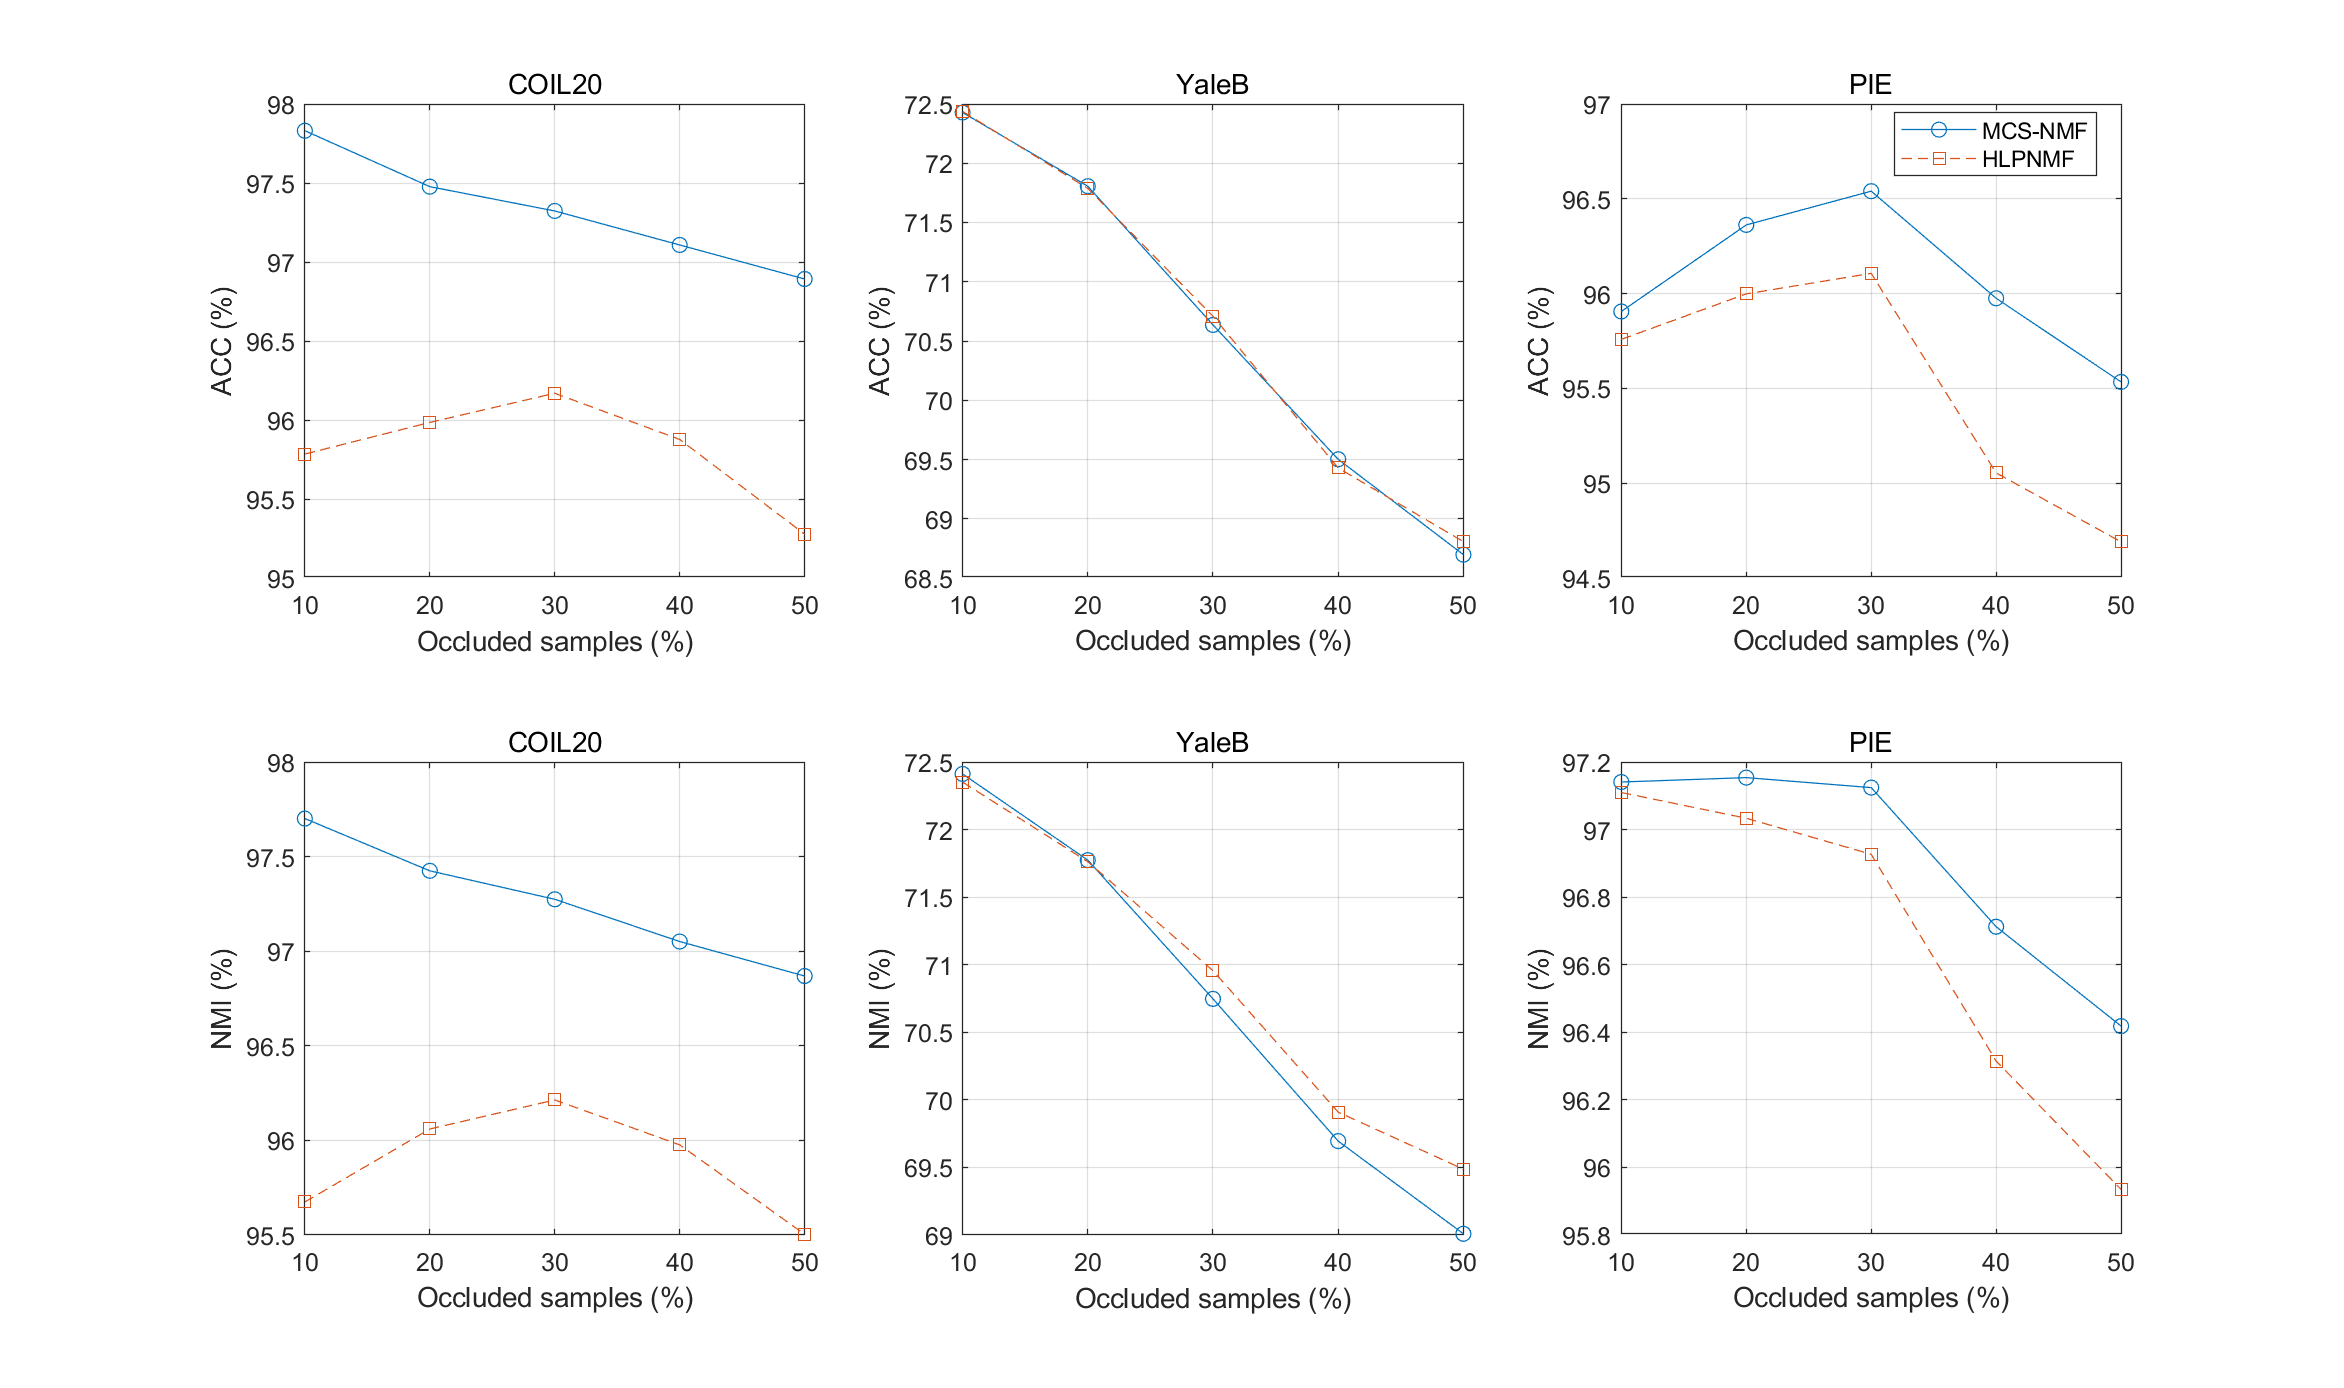
\includegraphics[width=0.94\textwidth]{block_robustness.png}
\caption{ACC and NMI under block occlusion on three image datasets.}
\label{fig:robustness}
\end{figure}

We further tested incorrect supervision by replacing $0\%$--$40\%$ of the labeled targets, within each class, by uniformly selected incorrect classes. The class-stratified $10\%$ labeled masks, corrupted targets, and initializations were paired across MCS-NMF, HLPNMF, SNMFWLP, and OCSNMF over 20 runs. Figures~\ref{fig:labelnoiseacc} and \ref{fig:labelnoisenmi} show that MCS-NMF achieves the strongest overall results on COIL20 and outperforms SNMFWLP and OCSNMF on PIE and YaleB. MCS-NMF and HLPNMF produce adjacent curves on PIE and YaleB. At $40\%$ label noise on MNIST, MCS-NMF records ACC of $87.93\%$ and NMI of $75.14\%$; HLPNMF records the highest scores at the largest corruption levels. The discrete class-wise corruption counts produce the small nonmonotonic changes on PIE and YaleB.

\begin{figure}[H]
\centering
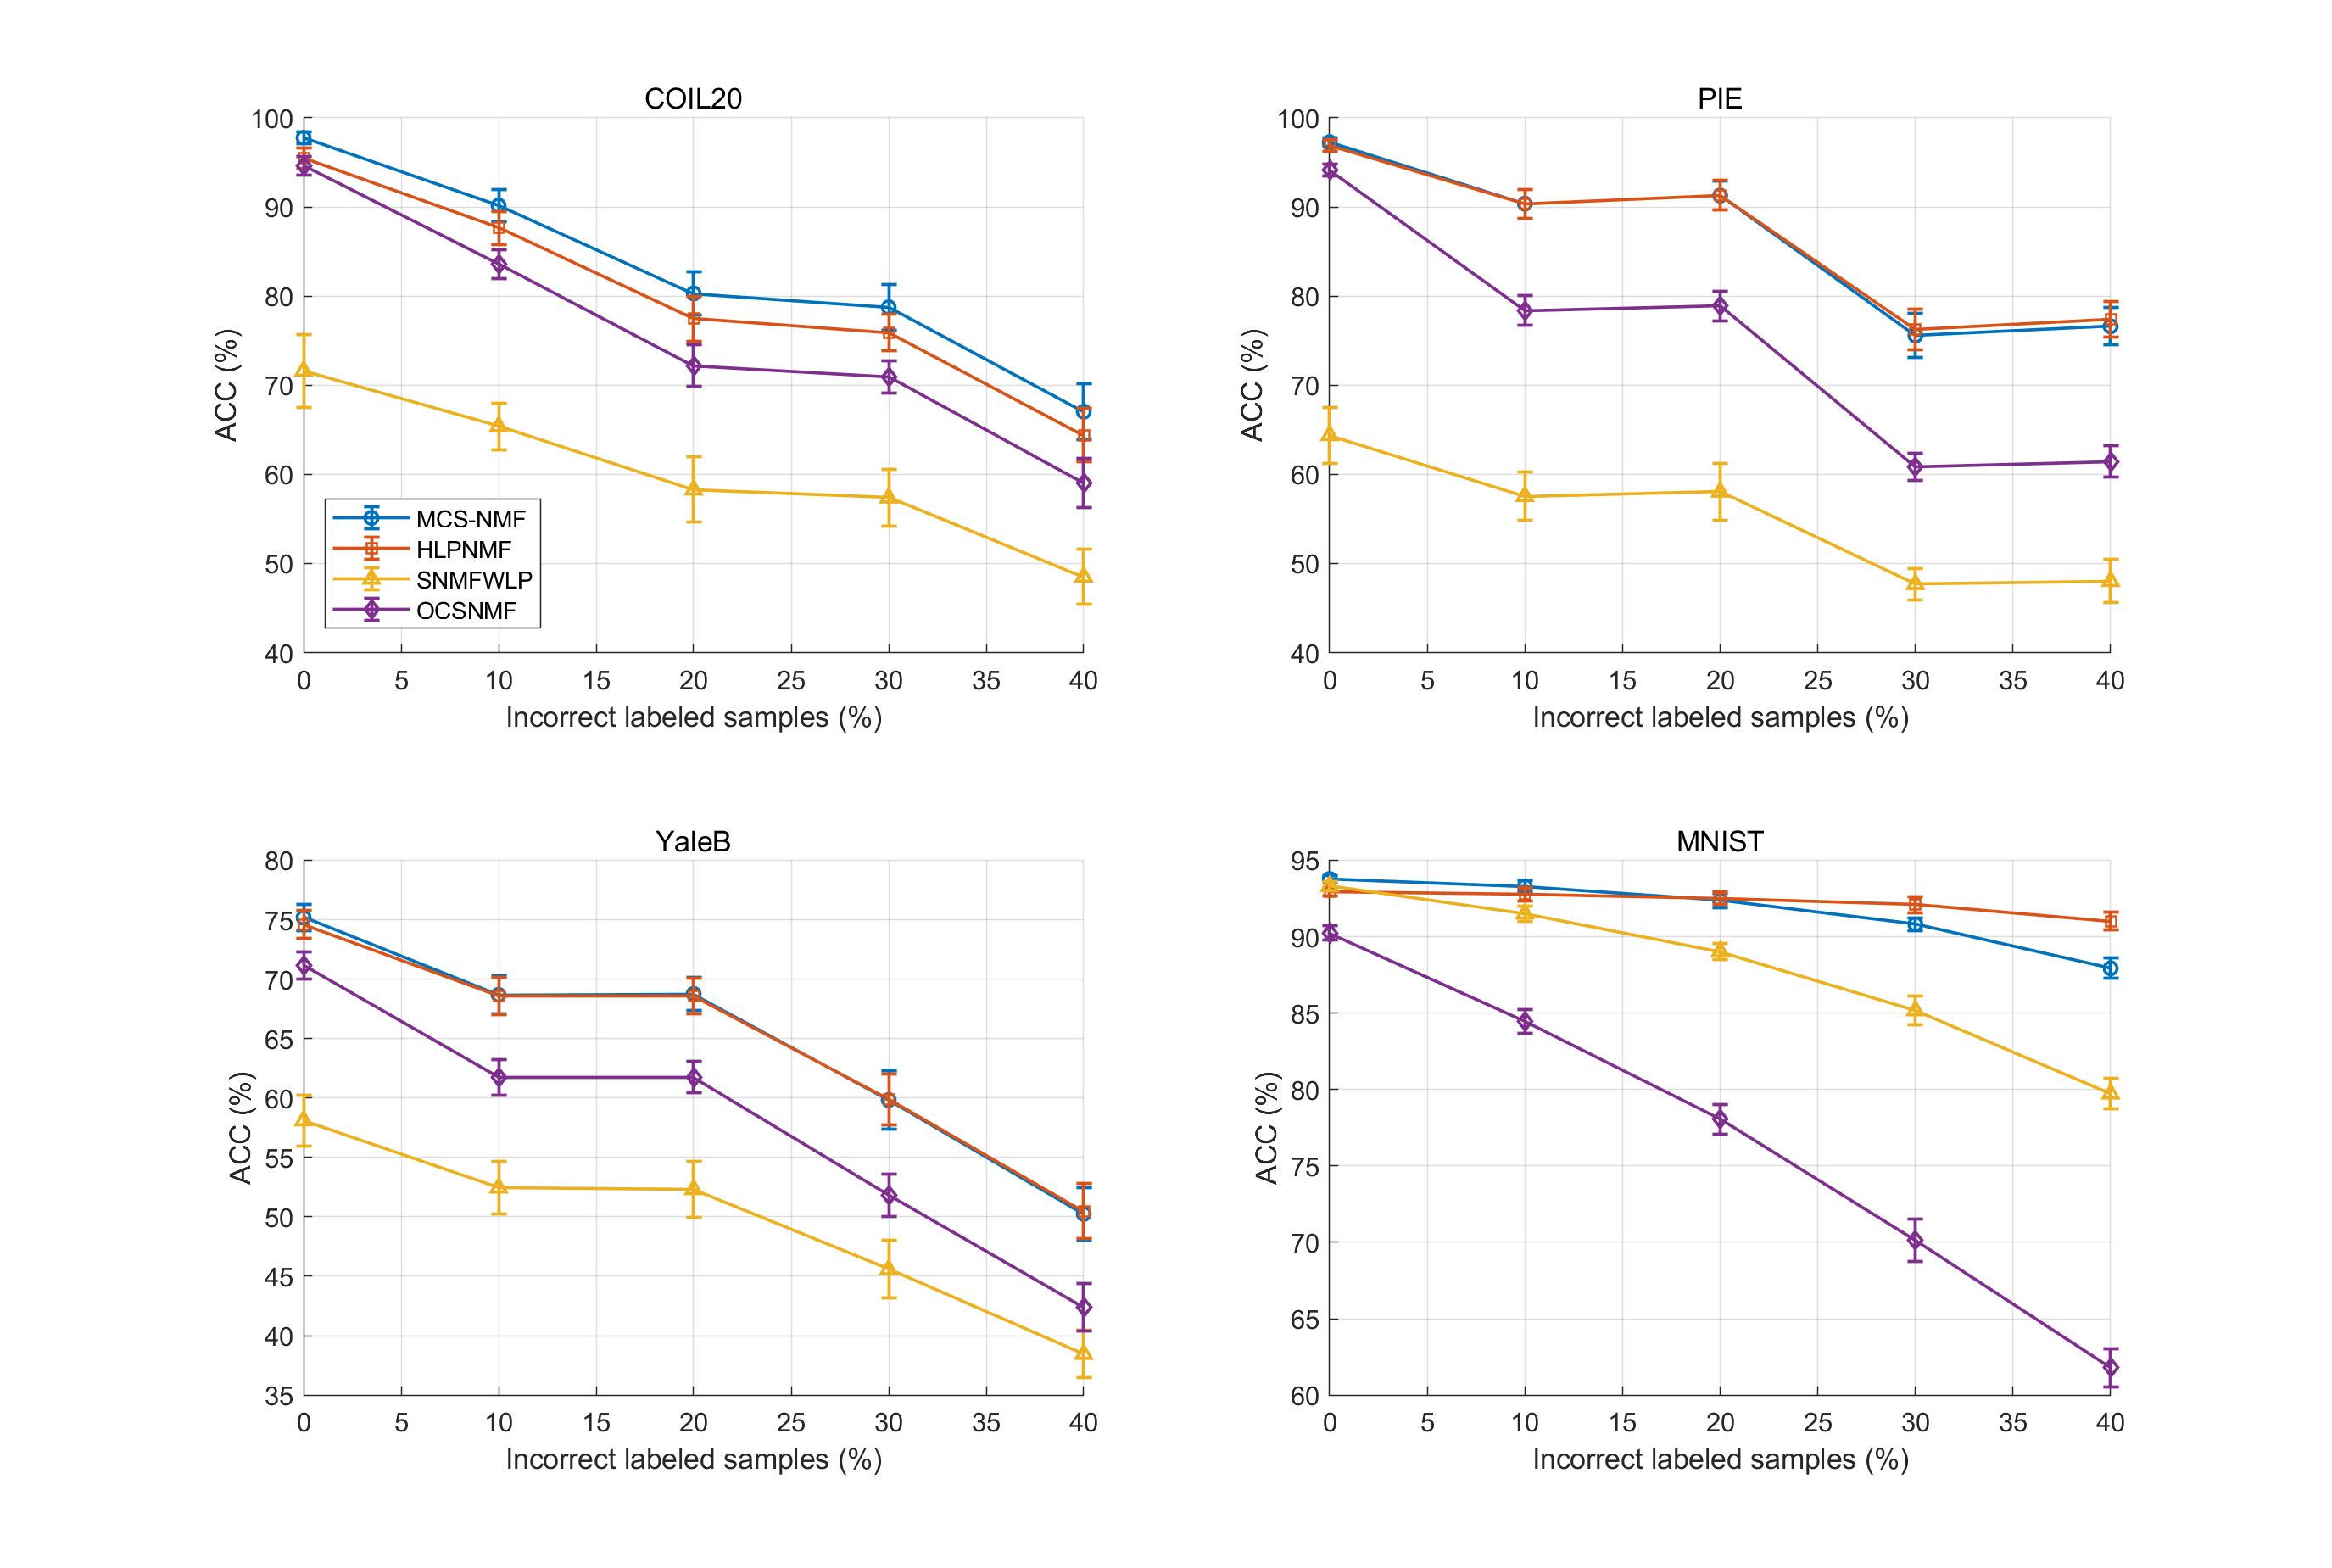
\includegraphics[width=0.82\textwidth]{label_noise_acc.png}
\caption{ACC under incorrect labels. Curves report means from 20 paired runs using common labeled masks and corrupted targets.}
\label{fig:labelnoiseacc}
\end{figure}

\begin{figure}[H]
\centering
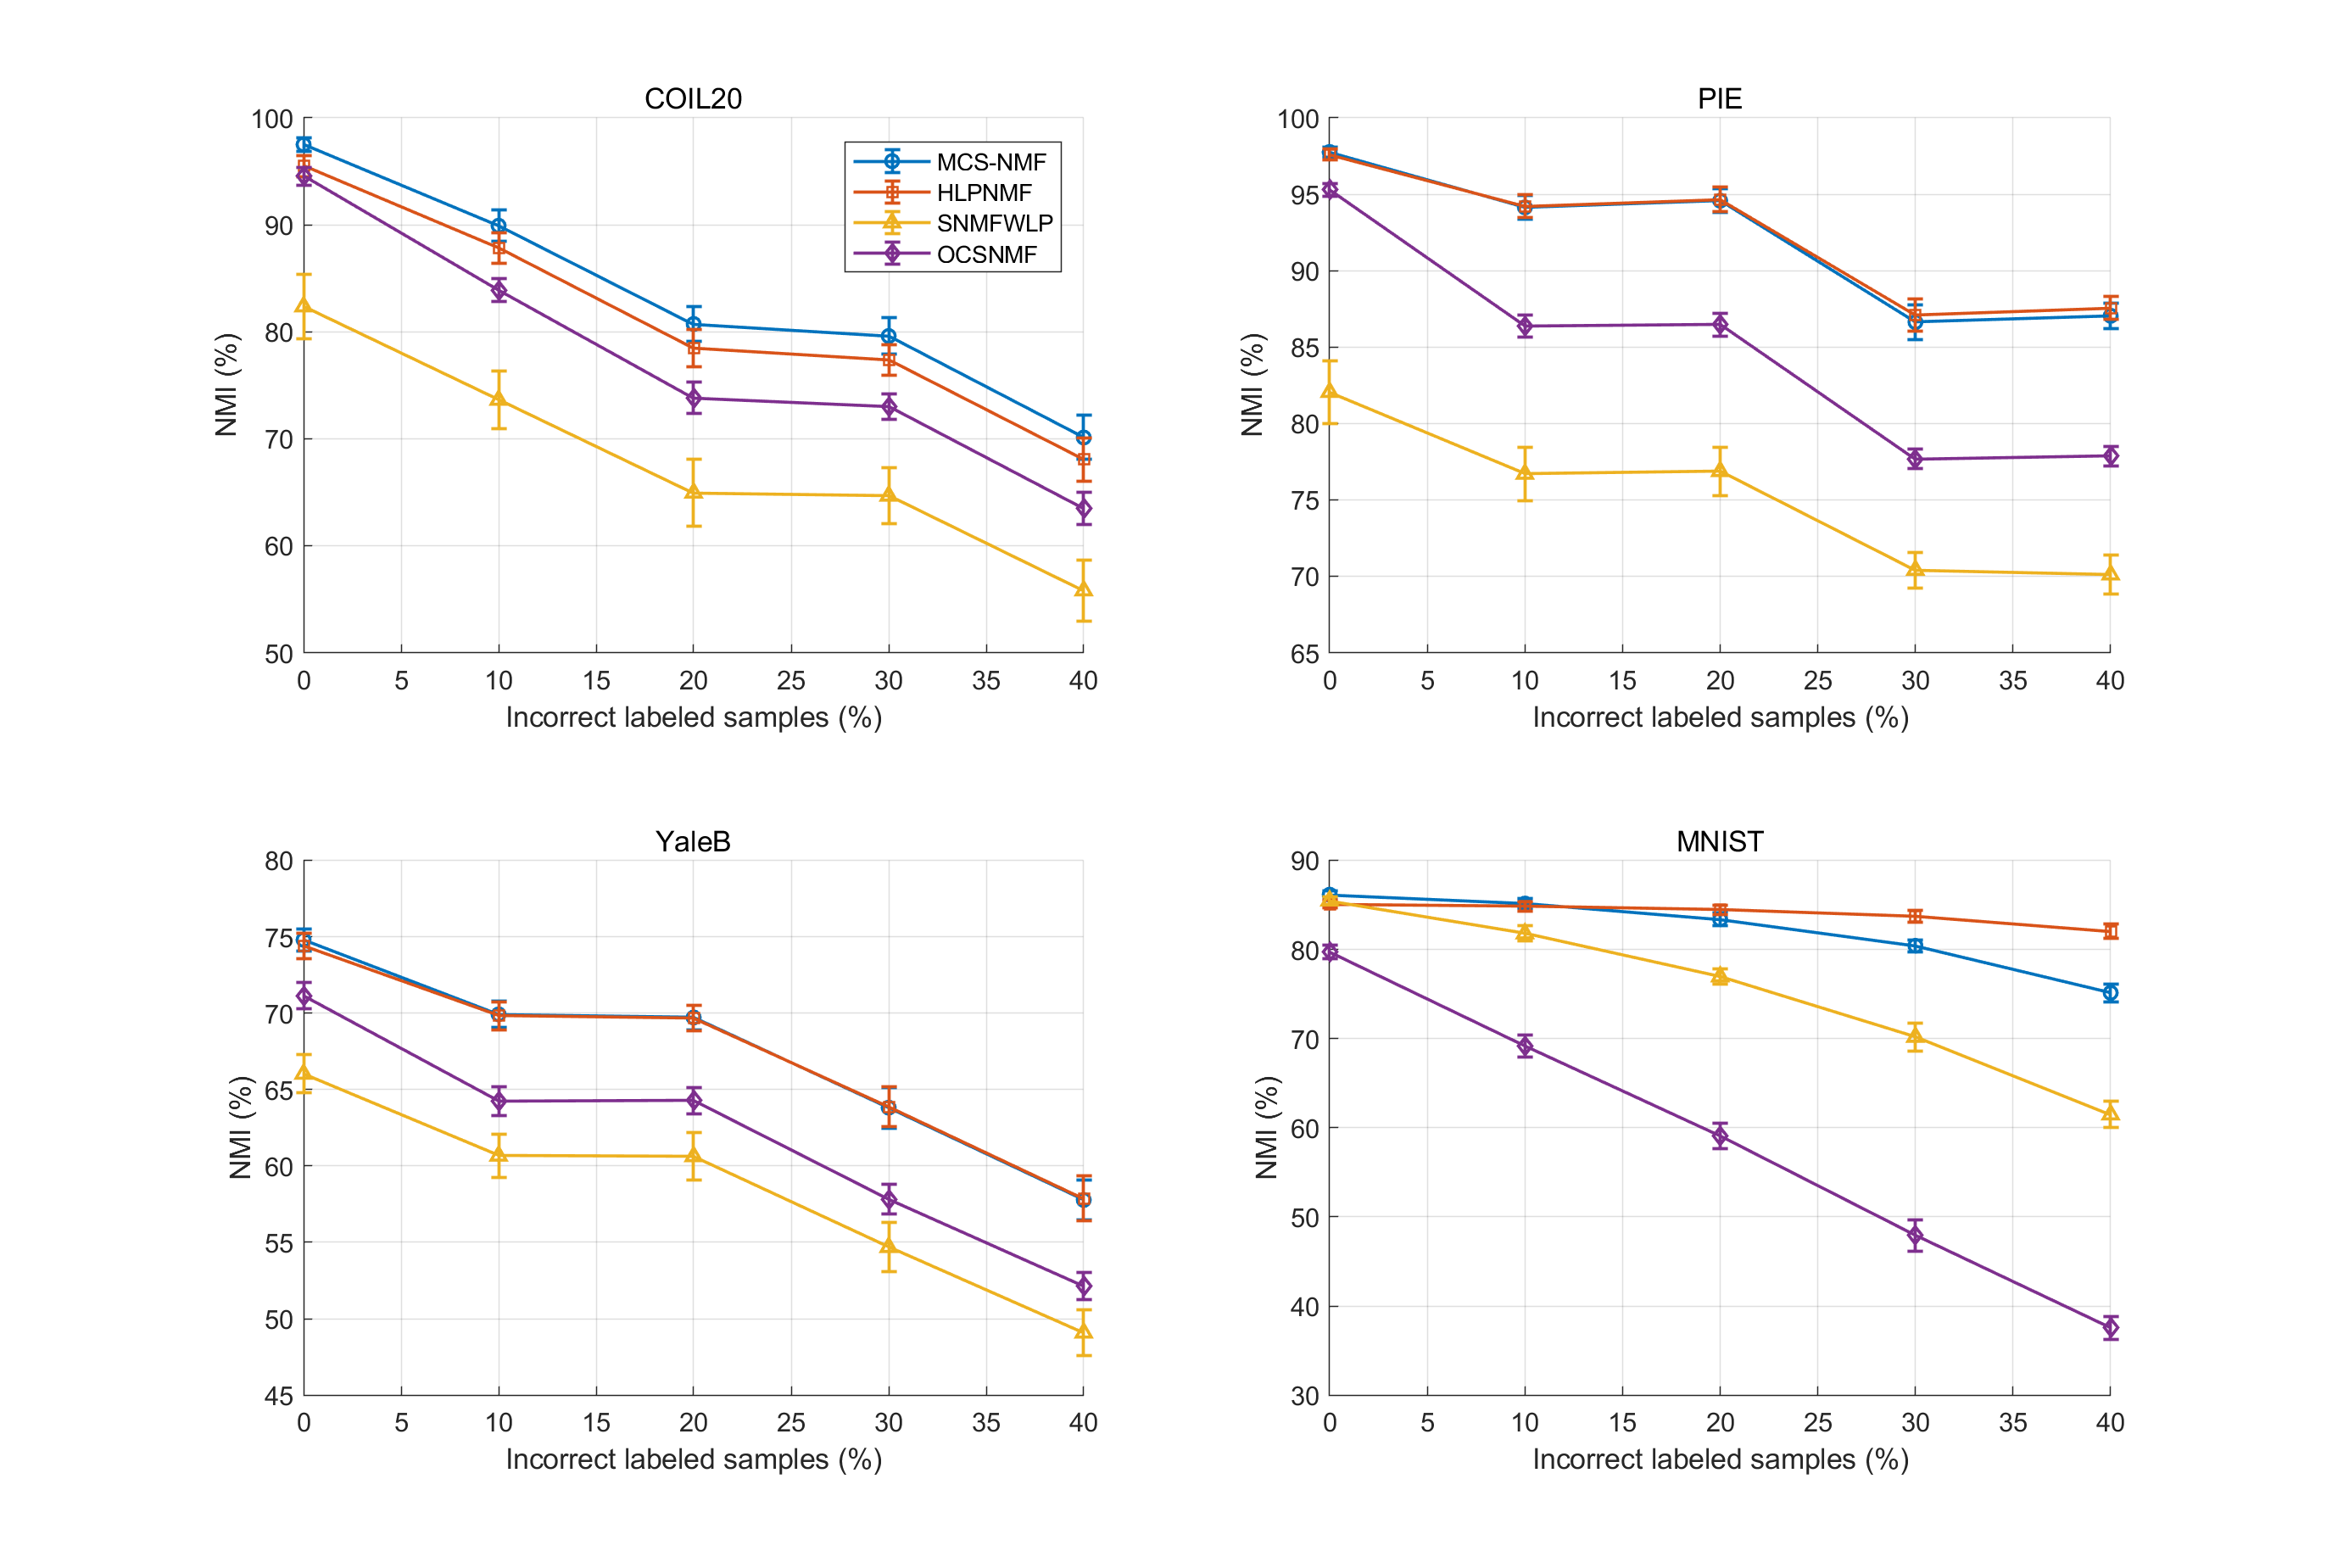
\includegraphics[width=0.82\textwidth]{label_noise_nmi.png}
\caption{NMI under incorrect labels under the protocol of Fig.~\ref{fig:labelnoiseacc}.}
\label{fig:labelnoisenmi}
\end{figure}

We next audited the aggregate class mass produced by HLPNMF under the same 20 paired labeled masks used in the main comparison. Figure~\ref{fig:massdrift}(a) reports total-variation distance from the labeled class prior. The labeled prior closely tracks the true unlabeled proportion, whereas HLPNMF produces excess mass drift on every dataset, reaching $19.53\%$ on AR, $8.46\%$ on YaleB, and $6.56\%$ on COIL100. MCS-NMF matches its prescribed target by construction. Within-dataset Spearman correlations between excess drift and clustering error exceed $0.5$ on six datasets [Fig.~\ref{fig:massdrift}(b)], connecting the controlled quantity directly to clustering behavior.

\begin{figure}[H]
\centering
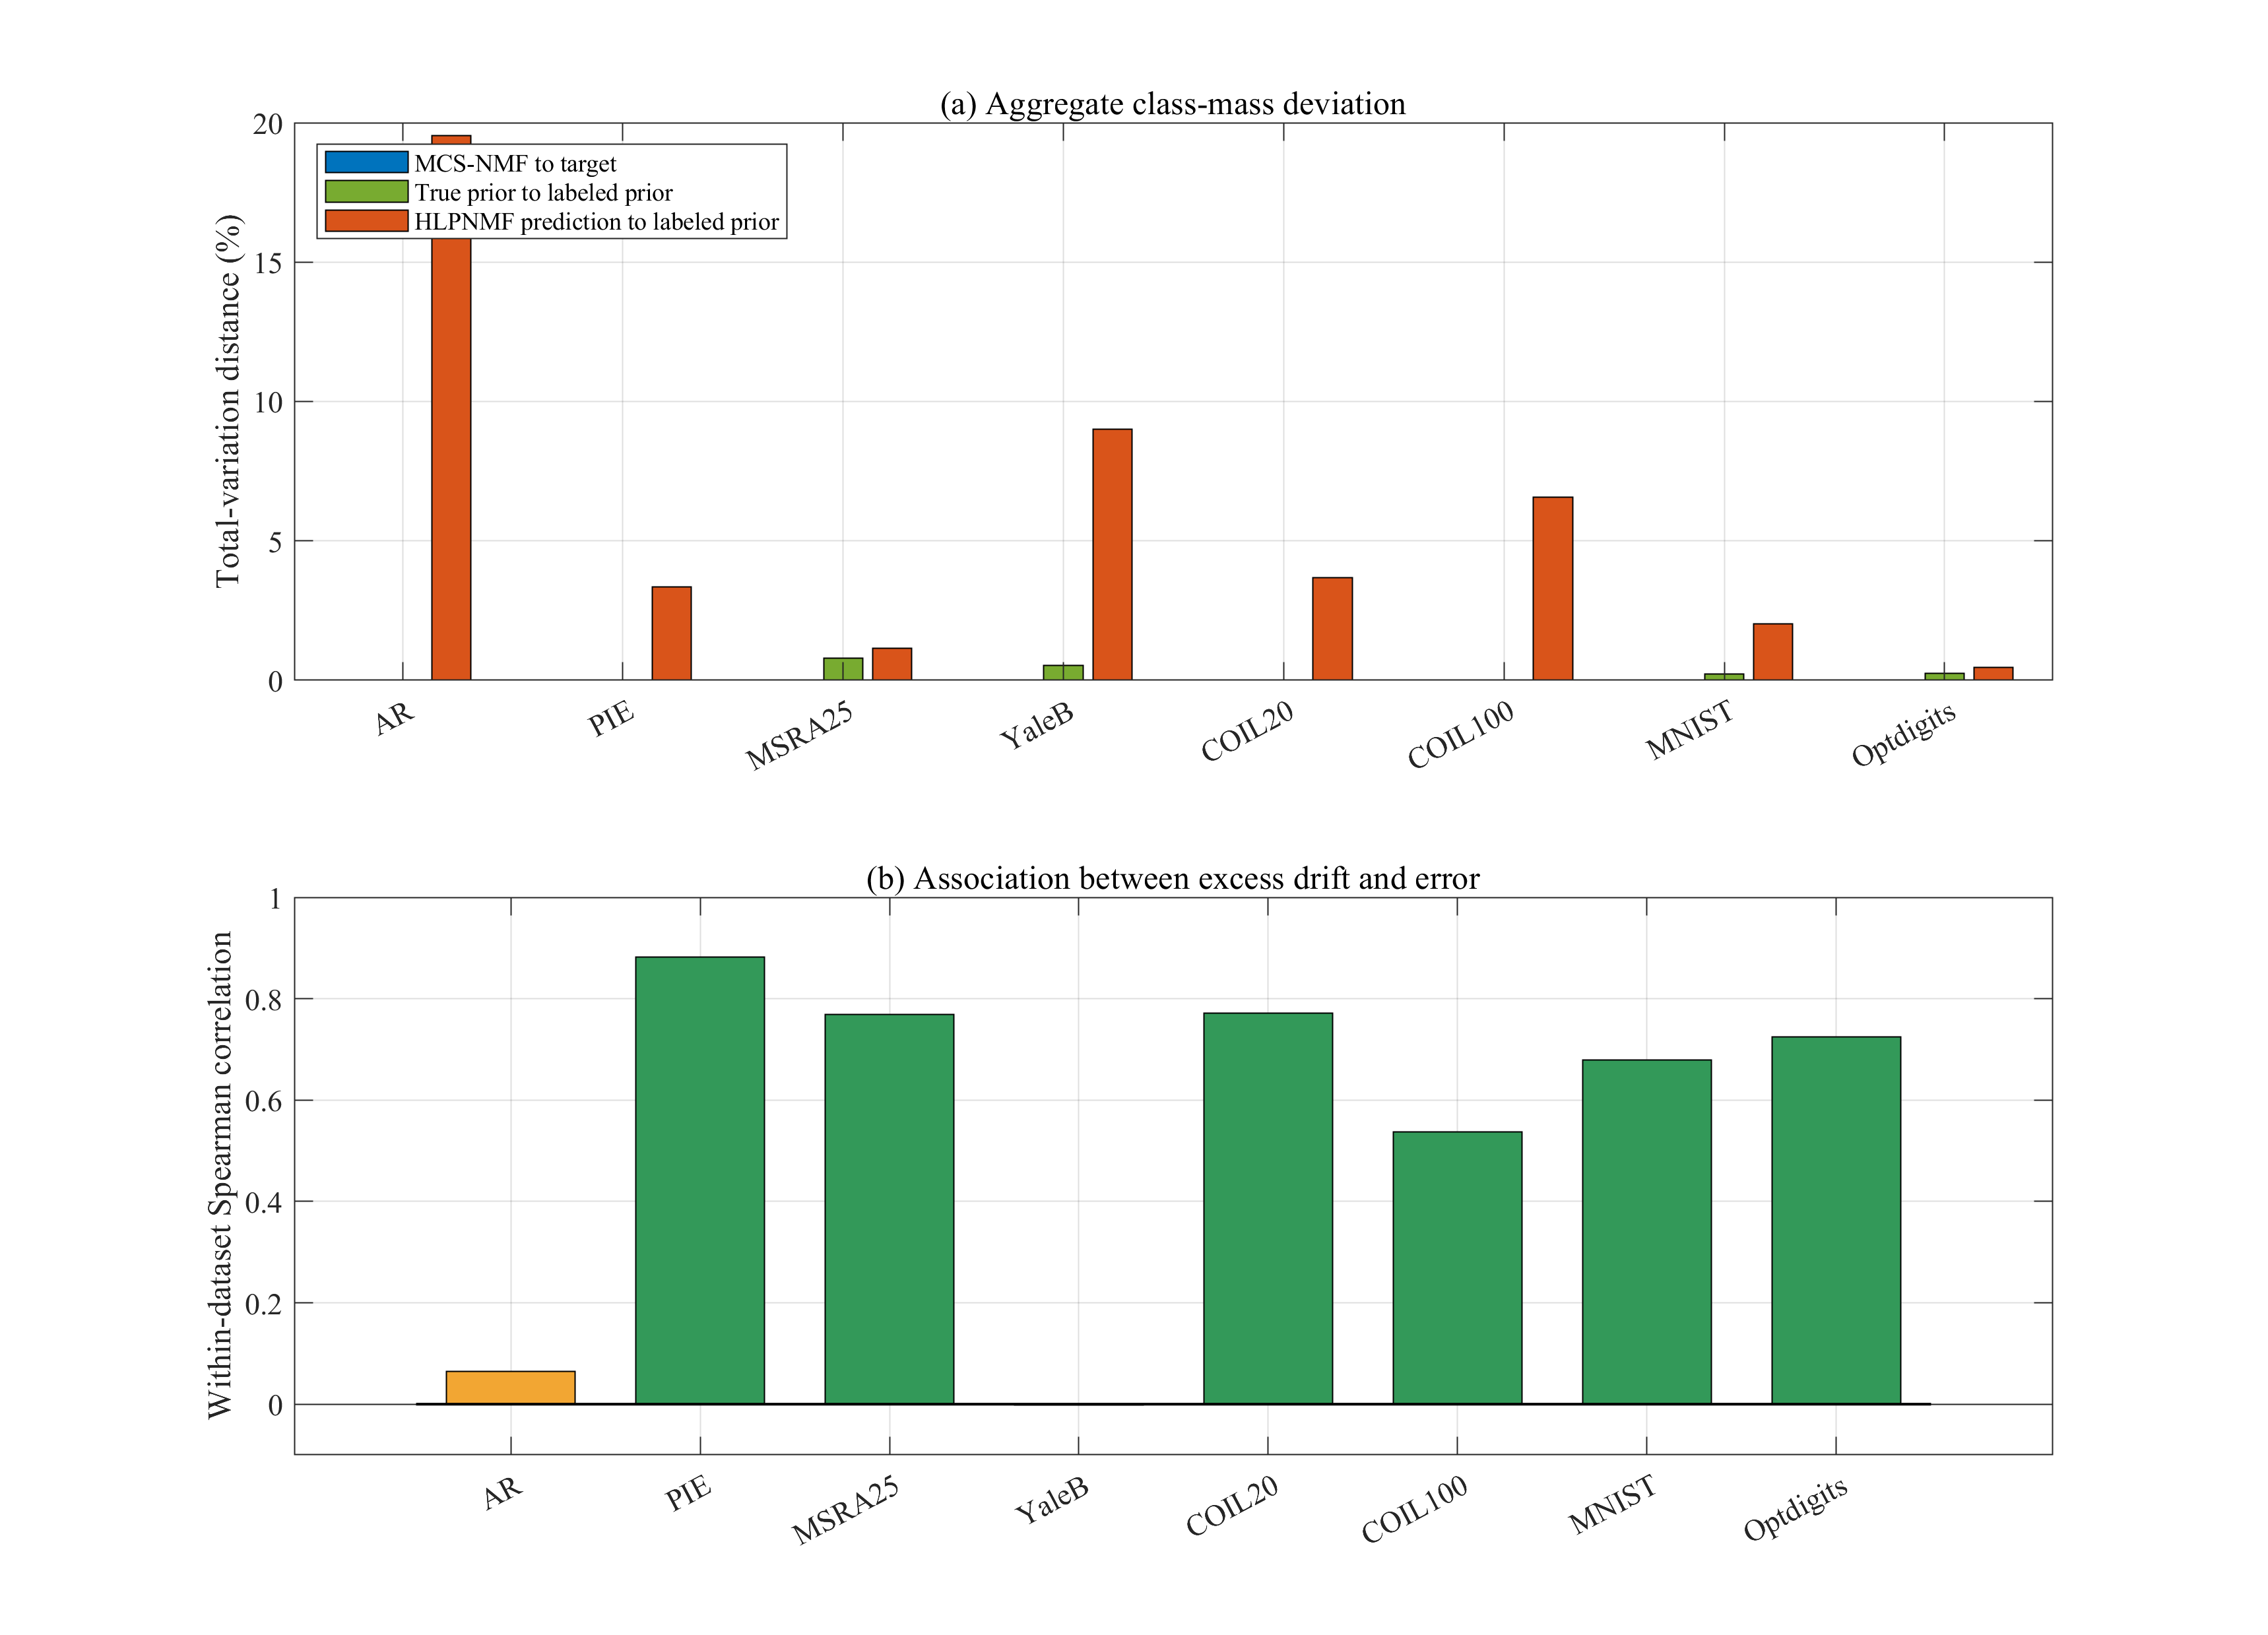
\includegraphics[width=\textwidth]{class_mass_drift.png}
\caption{Class-mass audit over 20 paired runs. (a) Deviation of the labeled prior from the true unlabeled proportion and deviation of predicted aggregate semantics from the labeled prior. (b) Within-dataset association between HLPNMF excess mass drift and clustering error.}
\label{fig:massdrift}
\end{figure}

Figure~\ref{fig:masstrajectory} traces the same quantity during optimization. MCS-NMF maintains the prescribed aggregate semantic mass throughout all accepted cycles. Under the identical labeled masks, HLPNMF drift increases from below $0.5\%$ to $7.9\%$ on COIL20 and to $10.0\%$ on PIE. The trajectories show that the global allocation distortion develops progressively during unconstrained propagation.

\begin{figure}[H]
\centering
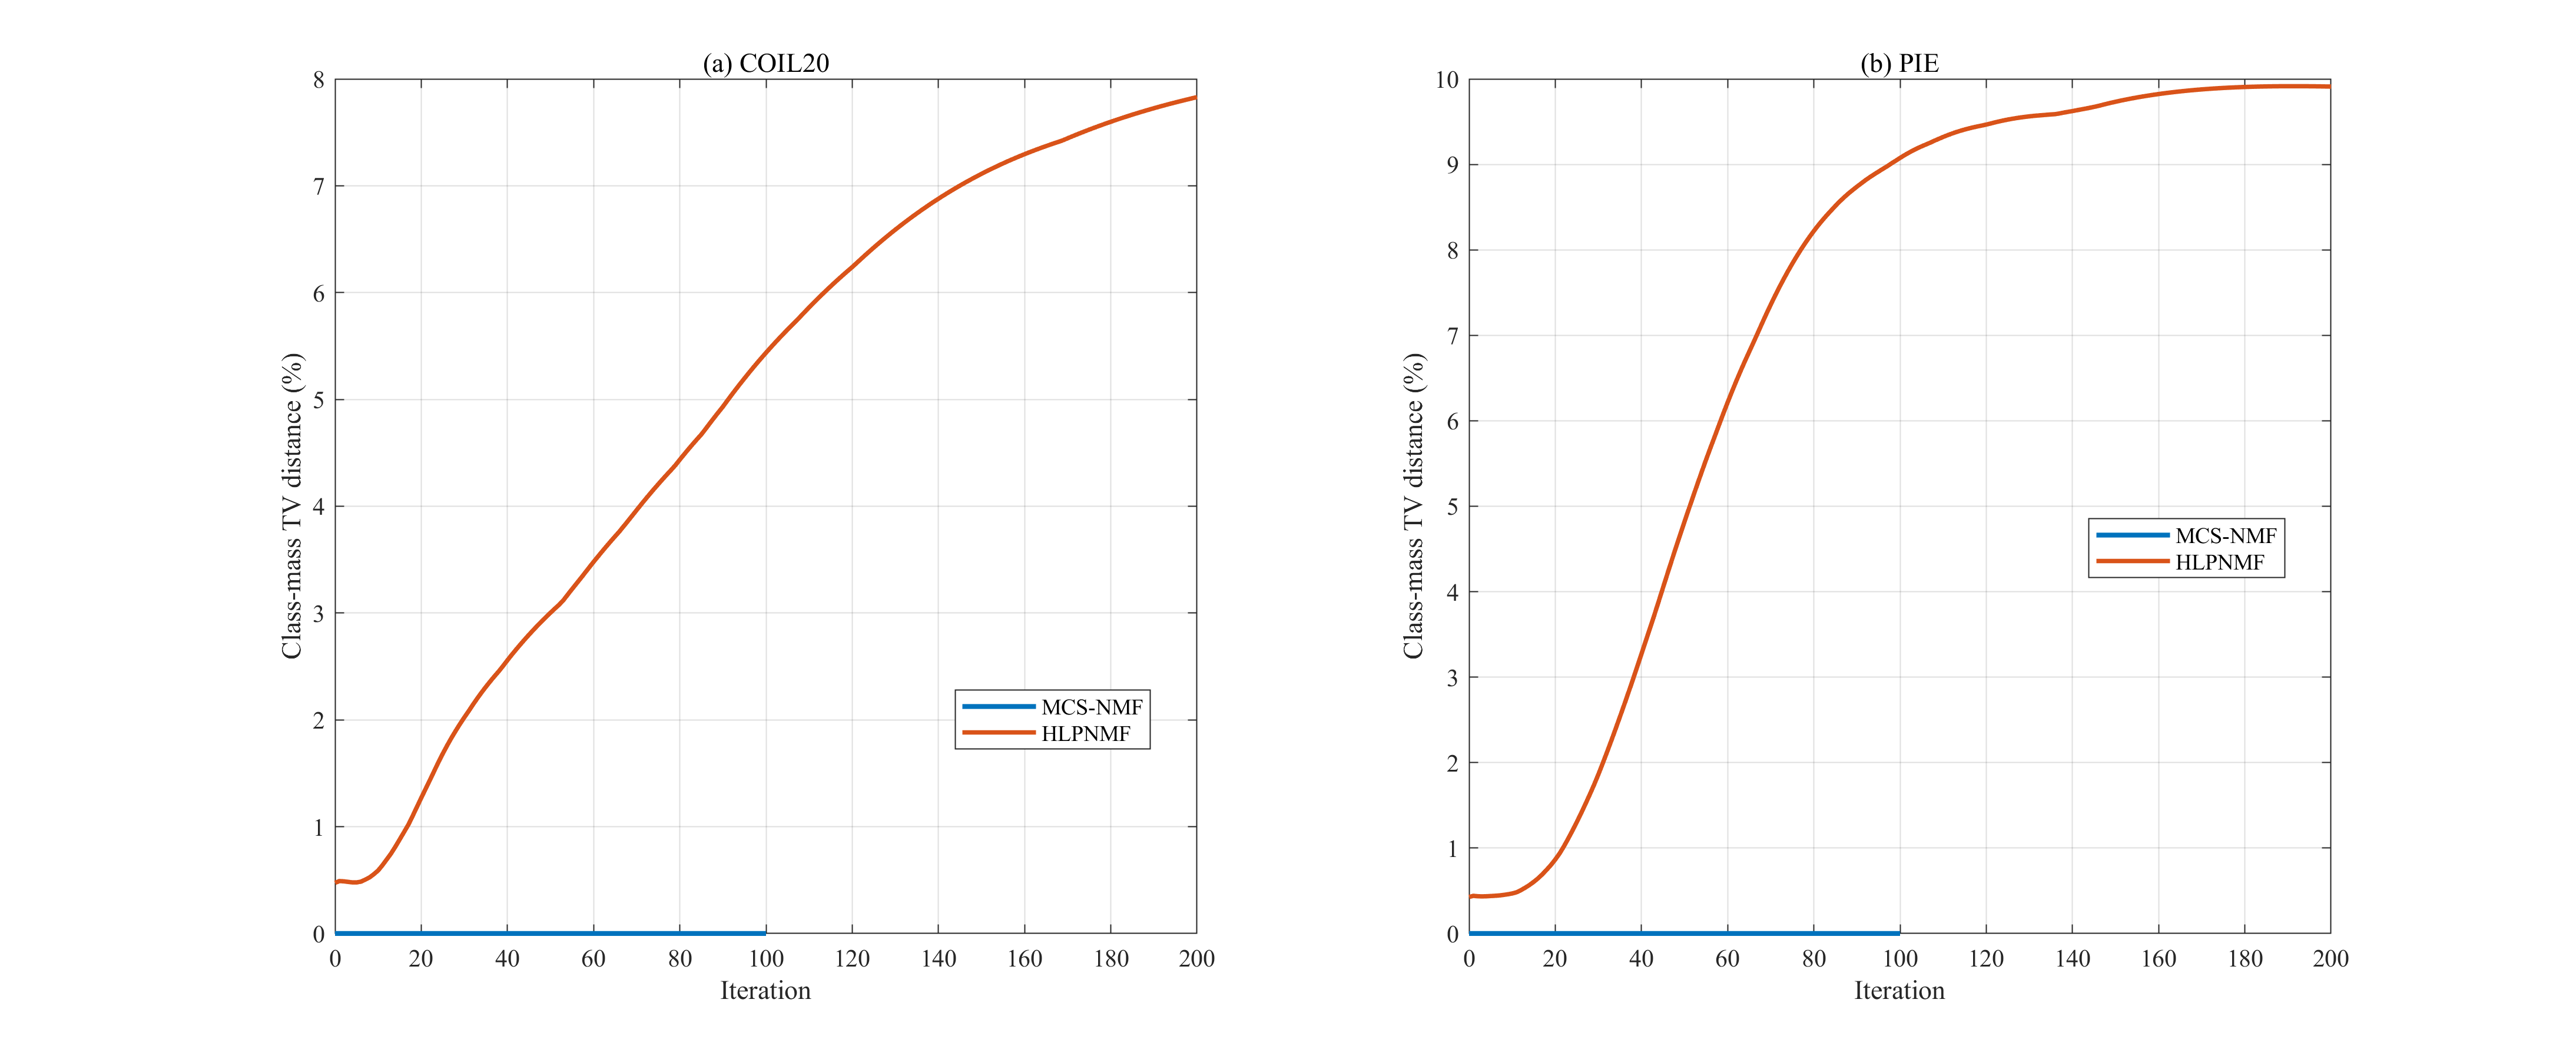
\includegraphics[width=\textwidth,trim=55 10 55 10,clip]{mass_trajectory.png}
\caption{Evolution of aggregate class-mass deviation on representative paired runs. Total-variation distance is measured from the labeled class prior after row normalization of the semantic coefficients.}
\label{fig:masstrajectory}
\end{figure}

Figure~\ref{fig:ablation} and Table~\ref{tab:controlled_ablation} isolate three components under the same labeled masks and five paired runs. The row-only variant removes the column marginal, the no-diffusion variant sets $\alpha=0$, and the first-order variant replaces the selected $k>1$ by $k=1$. The first two comparisons cover all eight core datasets; the propagation-order comparison uses the four datasets for which the selected full model has $k>1$. Diffusion contributes the largest mean change, while mass conservation and high-order propagation provide smaller positive gains. Because the target marginal is estimated from labeled samples, Fig.~\ref{fig:prior} additionally varies controlled prior bias.

\begin{figure}[!htbp]
\centering
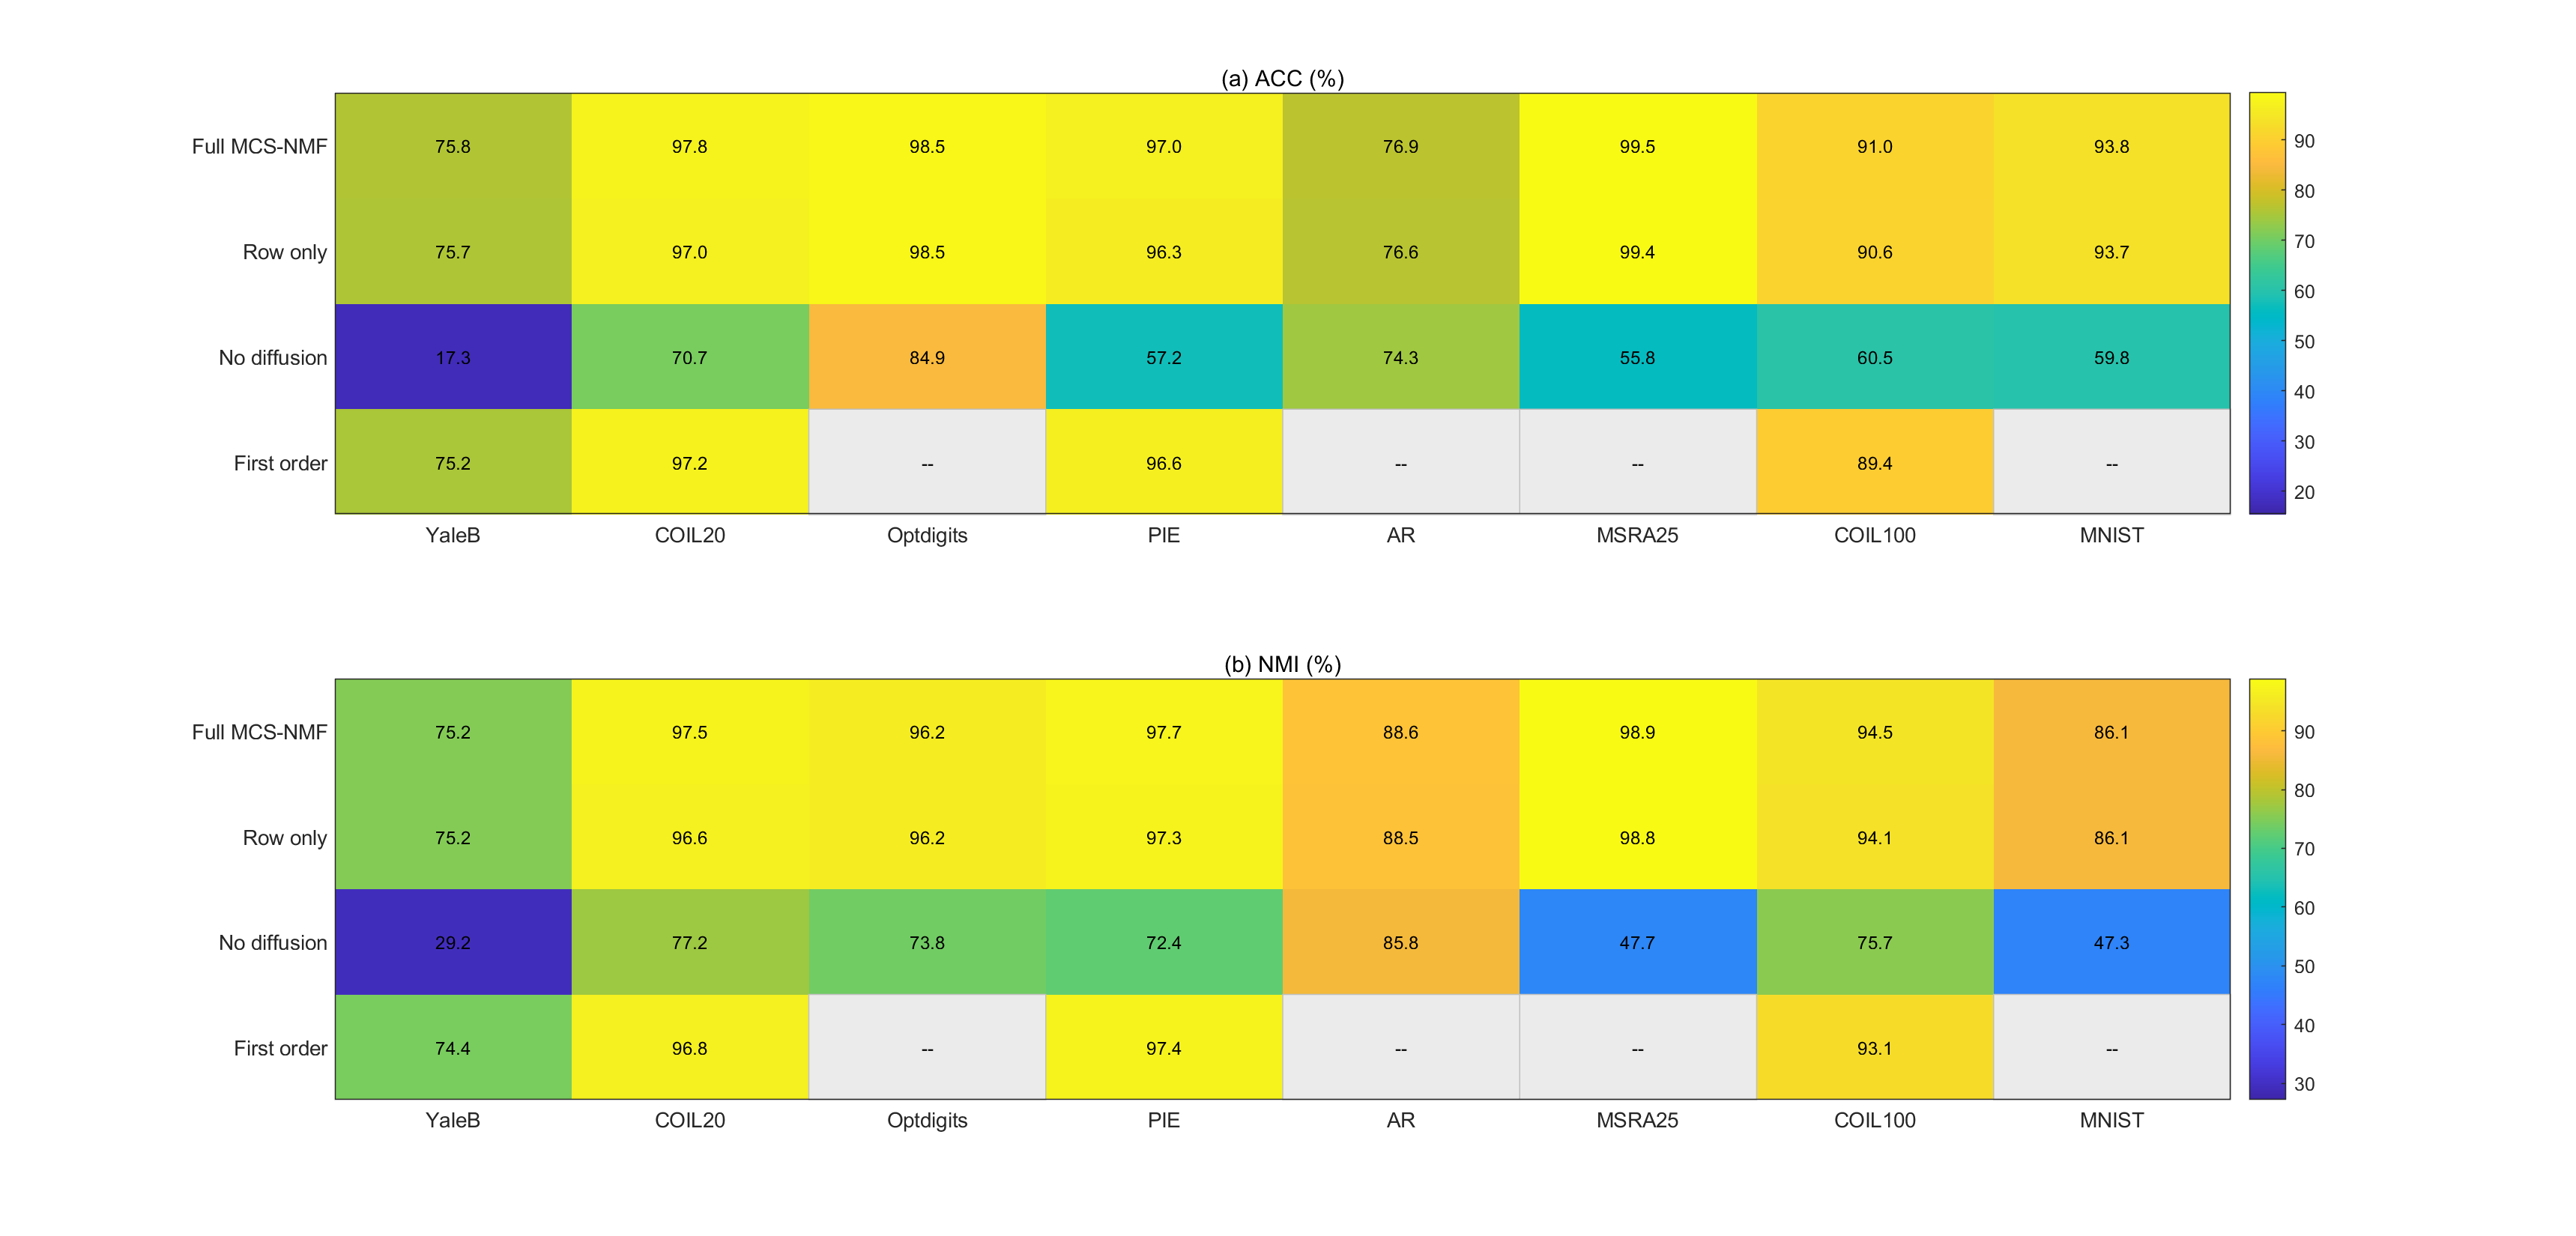
\includegraphics[width=0.98\textwidth]{controlled_ablation.png}
\caption{Controlled ablation of mass conservation, diffusion regularization, and propagation order. Dashes mark datasets whose selected full model already uses $k=1$.}
\label{fig:ablation}
\end{figure}

\begin{table}[!htbp]
\centering
\caption{Controlled ablation of the three MCS-NMF mechanisms. Gains are full-model minus ablated-model mean differences in percentage points.}
\label{tab:controlled_ablation}
\footnotesize
\begin{tabular}{llrrr}
\toprule
Factor & Comparison & Datasets & ACC gain & NMI gain \\
\midrule
Mass conservation & Row only $\rightarrow$ full & 8 & 0.309 & 0.212 \\
Diffusion regularization & No diffusion $\rightarrow$ full & 8 & 31.241 & 28.182 \\
High-order propagation & First order $\rightarrow$ selected order & 4 & 0.795 & 0.802 \\
\bottomrule
\end{tabular}
\end{table}


\begin{figure}[H]
\centering
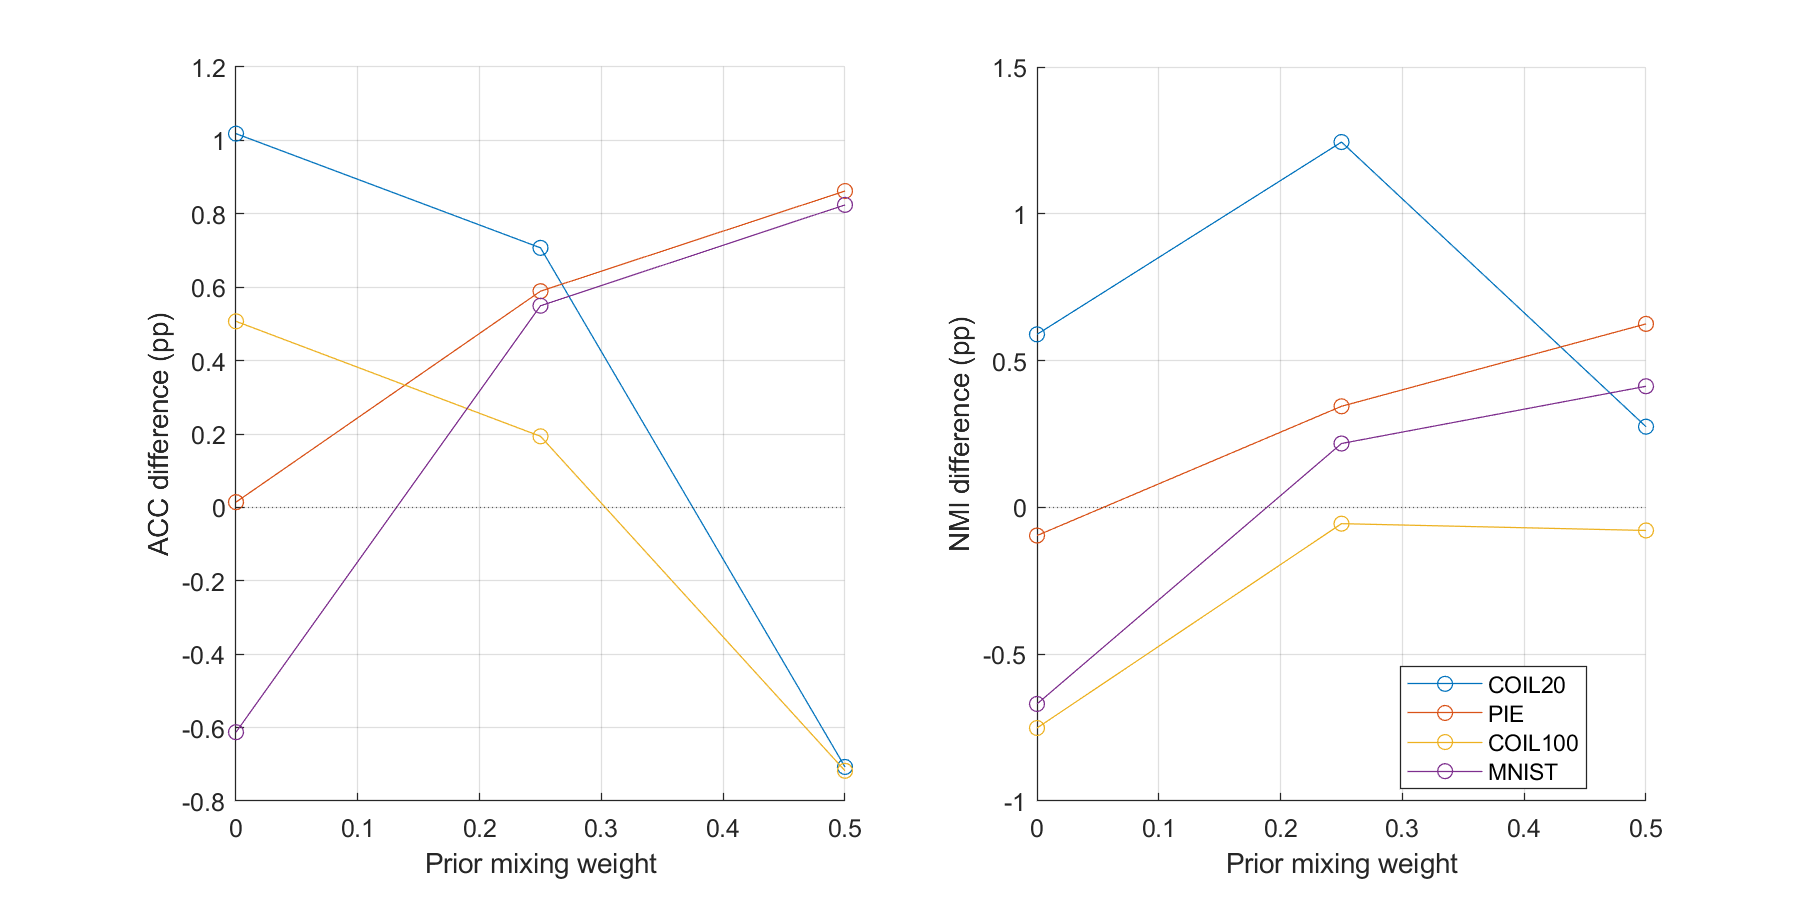
\includegraphics[width=0.88\textwidth]{prior_sensitivity.png}
\caption{Sensitivity of MCS-NMF to controlled perturbations of the class-mass prior.}
\label{fig:prior}
\end{figure}

We also evaluated class imbalance using exponential long-tail subsets whose smallest class retained one quarter of the samples in the largest class. The class-stratified $10\%$ supervision protocol and 20 paired runs were retained. Figure~\ref{fig:longtail} shows that MCS-NMF achieves the highest ACC, NMI, and macro-F1 on COIL20 and PIE. Its paired improvements over HLPNMF are $3.50$, $1.68$, and $4.94$ percentage points on COIL20 and $2.09$, $0.90$, and $2.77$ points on PIE; all six $95\%$ bootstrap intervals exclude zero. On MNIST, SNMFWLP achieves the highest four metrics, followed by MCS-NMF in ACC, NMI, and macro-F1. OCSNMF and SNMFWLP obtain higher tail-class recall on several conditions. The result separates overall partition quality from minority-class recovery under a strongly skewed class distribution.

\begin{figure}[H]
\centering
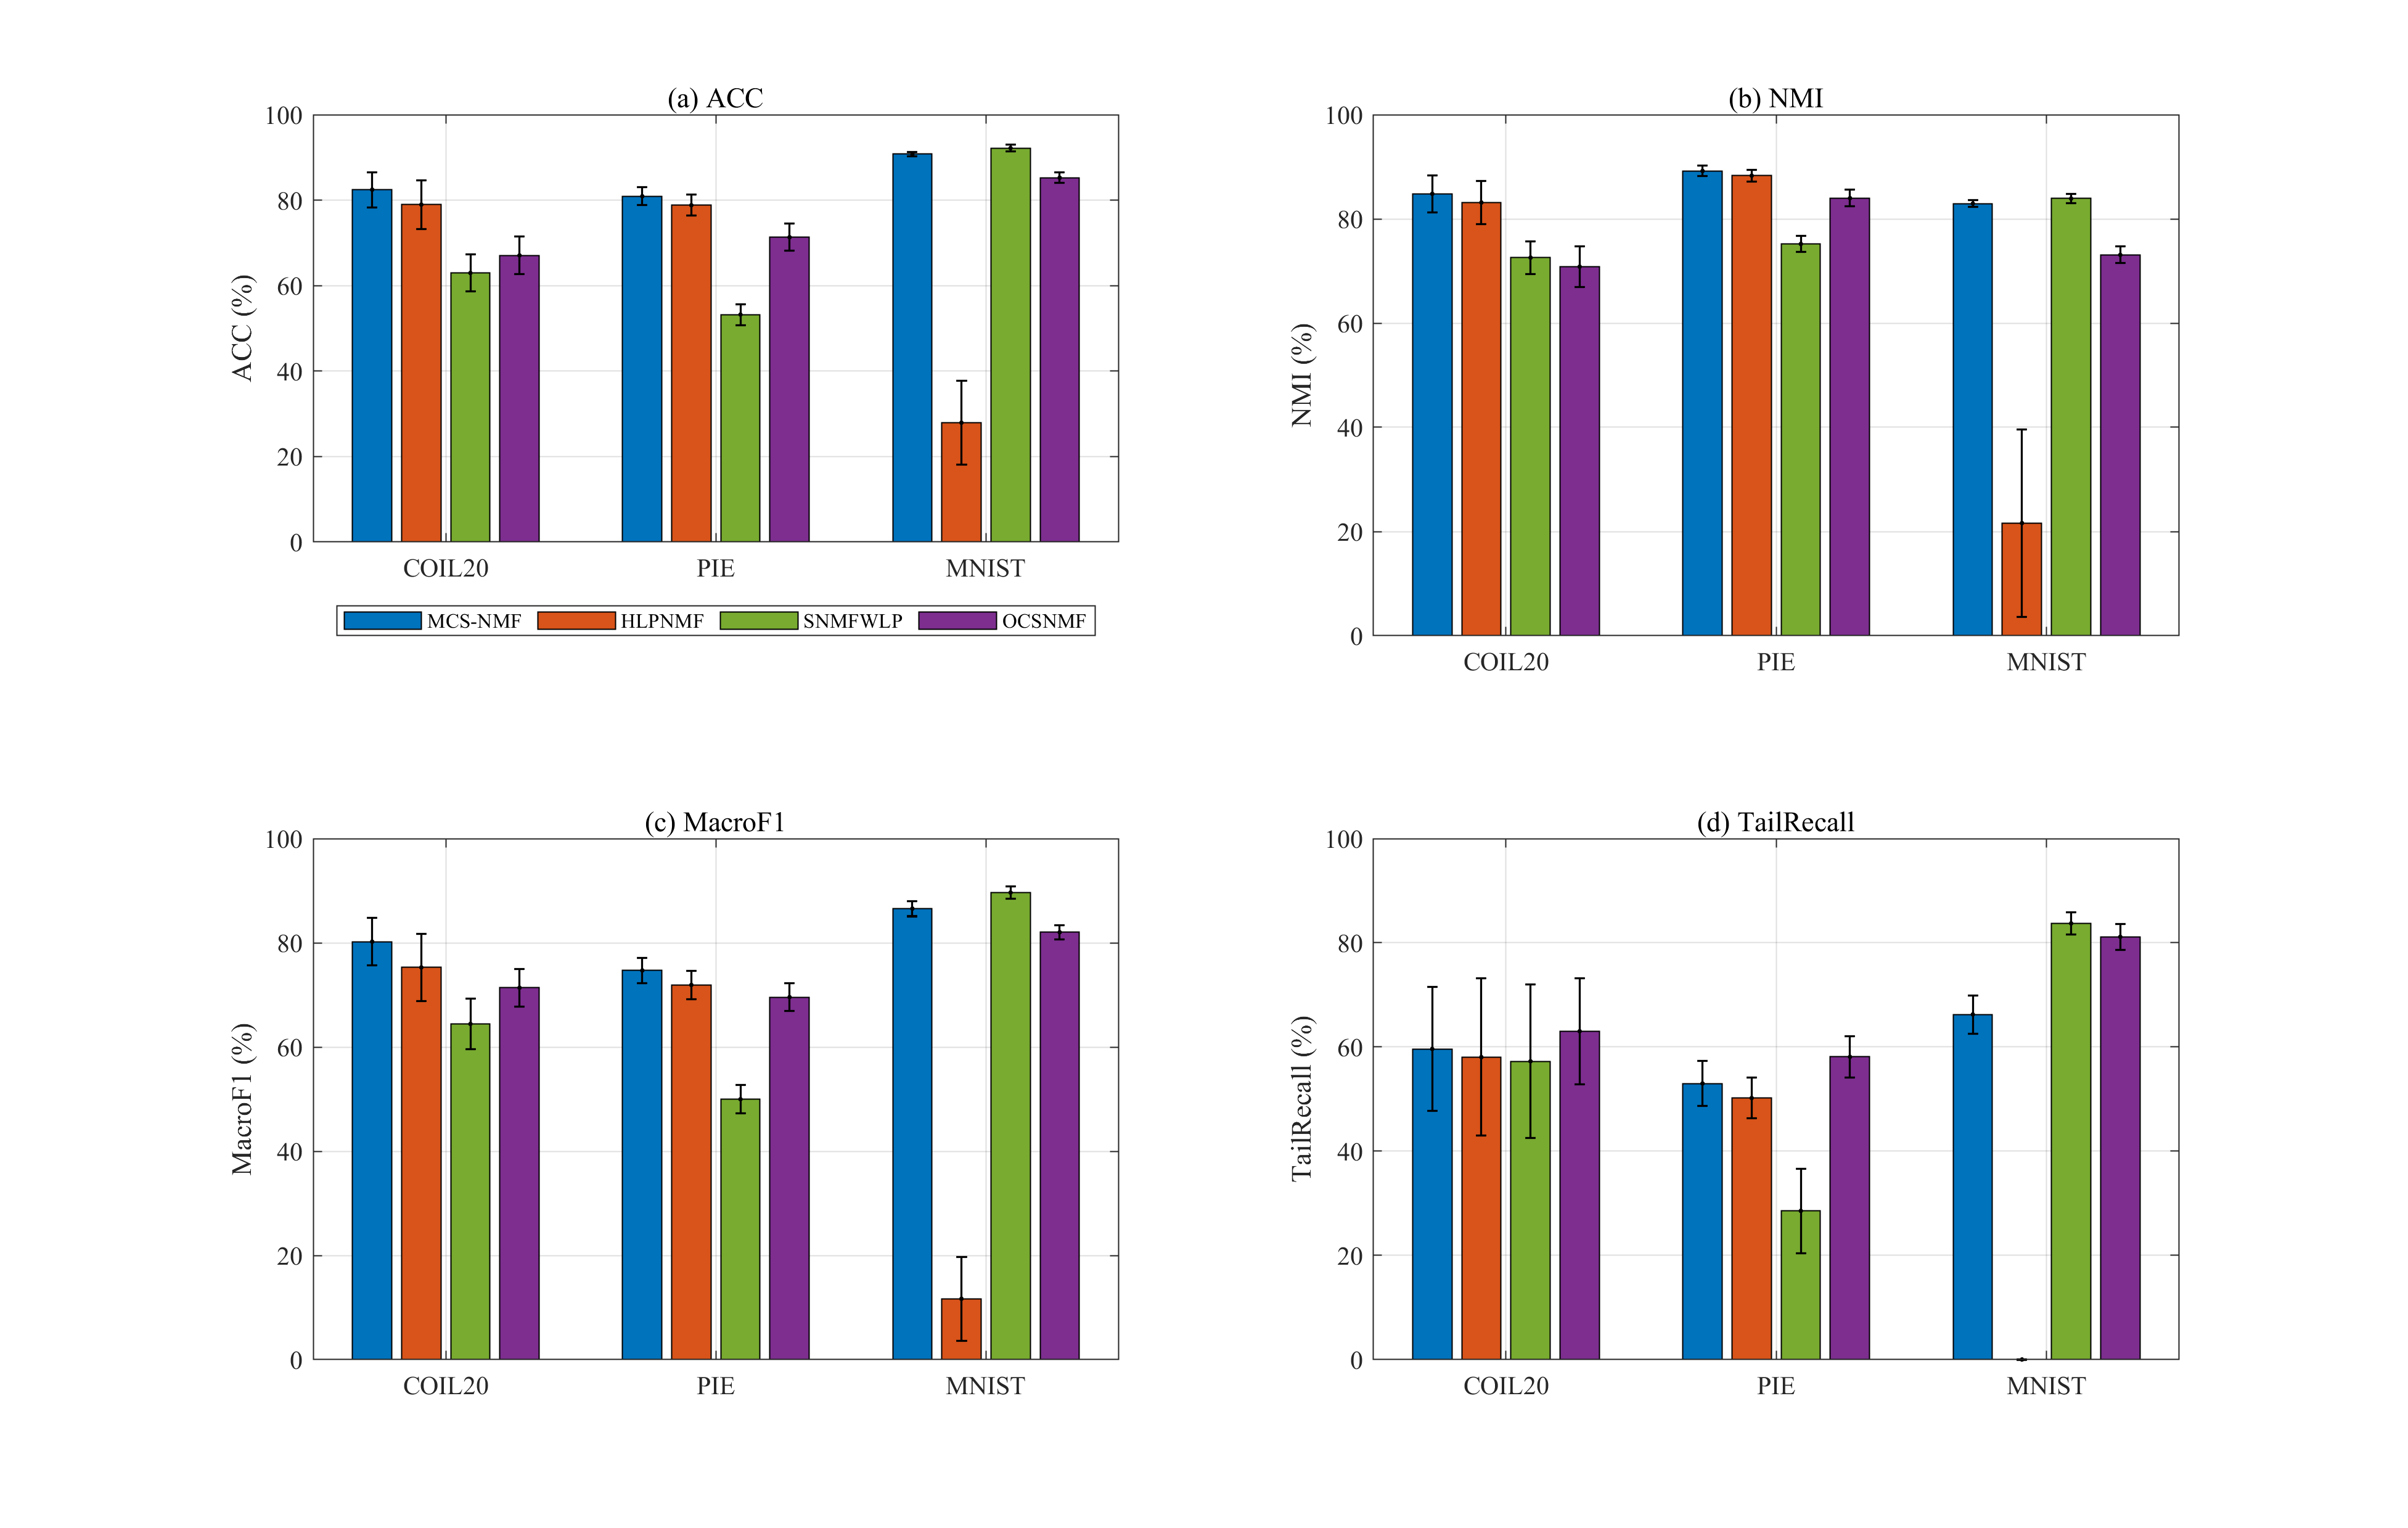
\includegraphics[width=\textwidth]{longtail_comparison.png}
\caption{Long-tail clustering under a $4{:}1$ head-to-tail sample ratio. Bars and error bars report means and standard deviations over 20 paired runs. Tail recall averages recall over the smallest quarter of classes.}
\label{fig:longtail}
\end{figure}

\subsection{Scalability and runtime}

Using the available PIE benchmark, we formed nested subsets containing 420, 840, 1680, and 2856 samples from 10, 20, 40, and 68 classes. Figure~\ref{fig:scaling} compares MCS-NMF with SPNMF and GOCNMF using identical subsets and paired labeled masks. MCS-NMF retains ACC above $96\%$ and NMI above $97\%$ at every scale; GOCNMF remains above $94\%$ on both metrics, whereas SPNMF declines as the number of classes increases. MCS-NMF runtime grows from 1.86 to 33.64 seconds, stored graph arrays from 0.44 to 3.75 MiB, and transition-structure sparsity from $91.57\%$ to $98.16\%$. Table~\ref{tab:runtime} compares nine methods using end-to-end timings that include graph construction, optimization, and the native decision step. MCS-NMF is faster than HLPNMF on COIL100, MNIST, and Optdigits and faster than SPNMF and CSDCP on every dataset. Its additional class-mass and semantic optimization makes it slower than the simpler LP, GOCNMF, OCSNMF, and LpCNMF pipelines.

\begin{figure}[H]
\centering
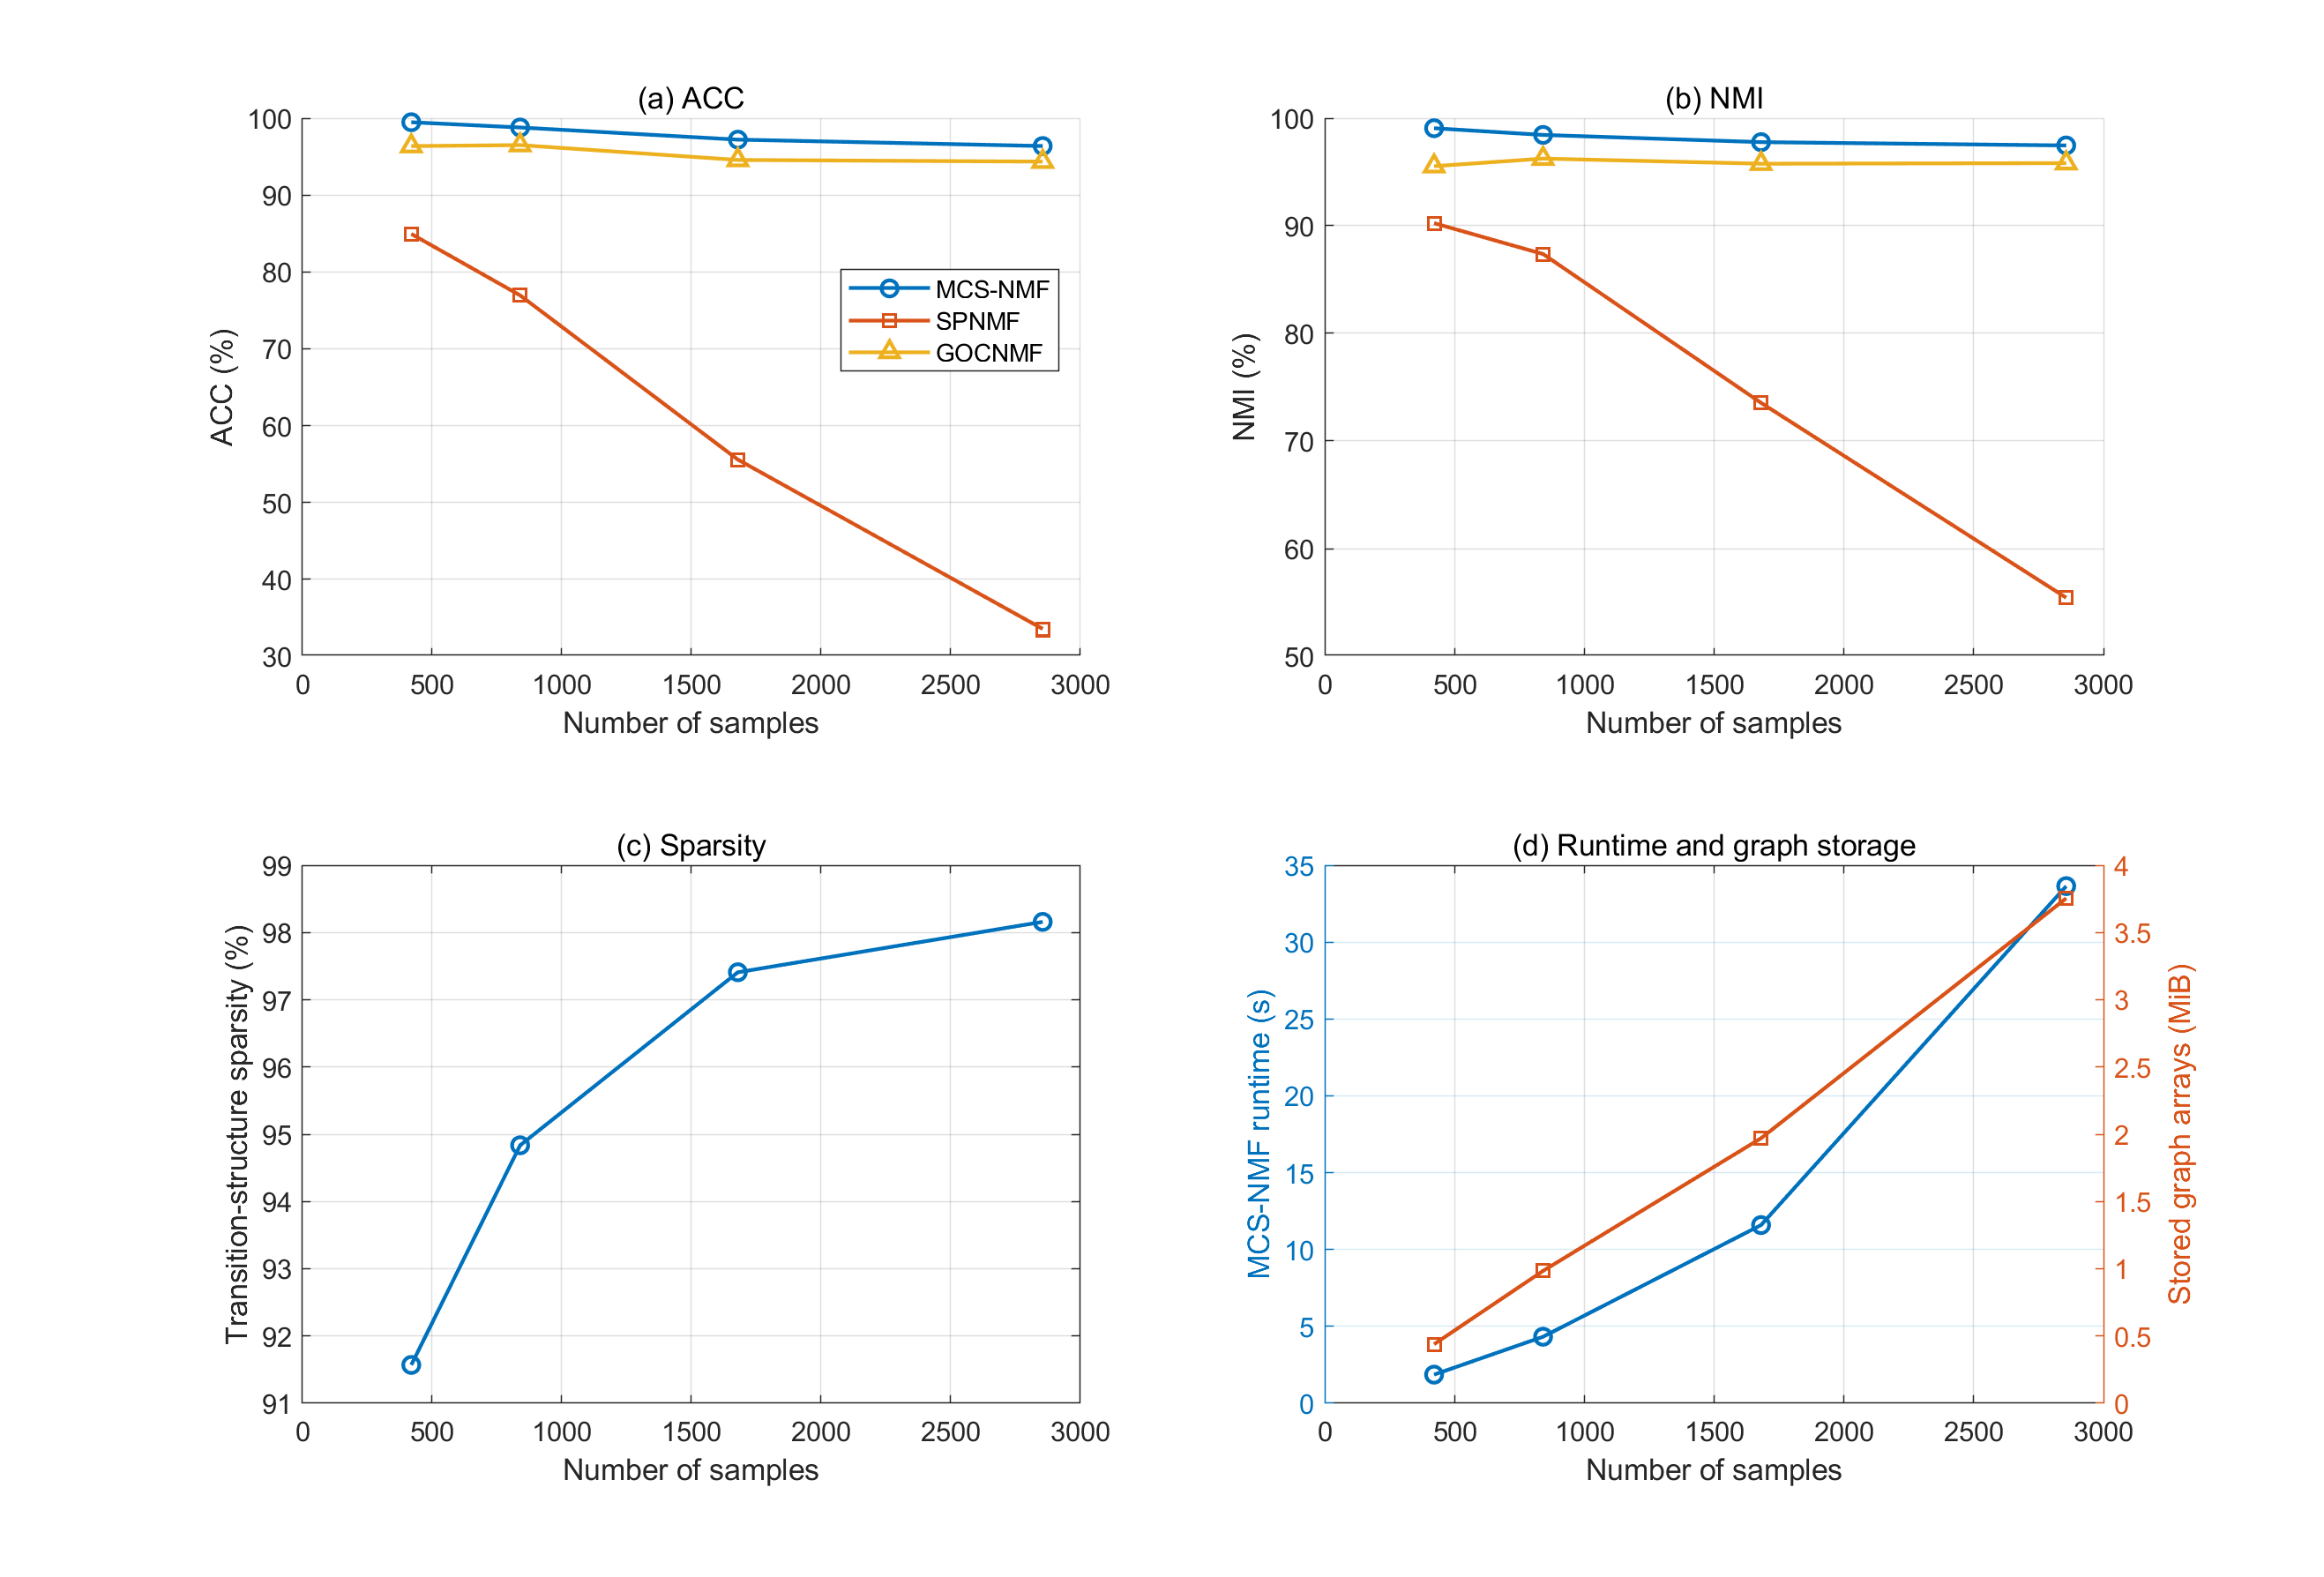
\includegraphics[width=0.90\textwidth]{pie_scaling_reference.png}
\caption{PIE scalability. ACC and NMI compare MCS-NMF with SPNMF and GOCNMF; the lower panels report MCS-NMF transition sparsity, runtime, and stored graph-array size.}
\label{fig:scaling}
\end{figure}

The empirical scaling trend agrees with the operation-count analysis. Across the four PIE subsets, the logarithm of measured runtime has correlation $0.994$ with the logarithm of the normalized complexity proxy, and the fitted runtime slope with respect to $n$ is $1.49$. Figure~\ref{fig:complexityruntime} confirms the predicted growth trend.

\begin{figure}[H]
\centering
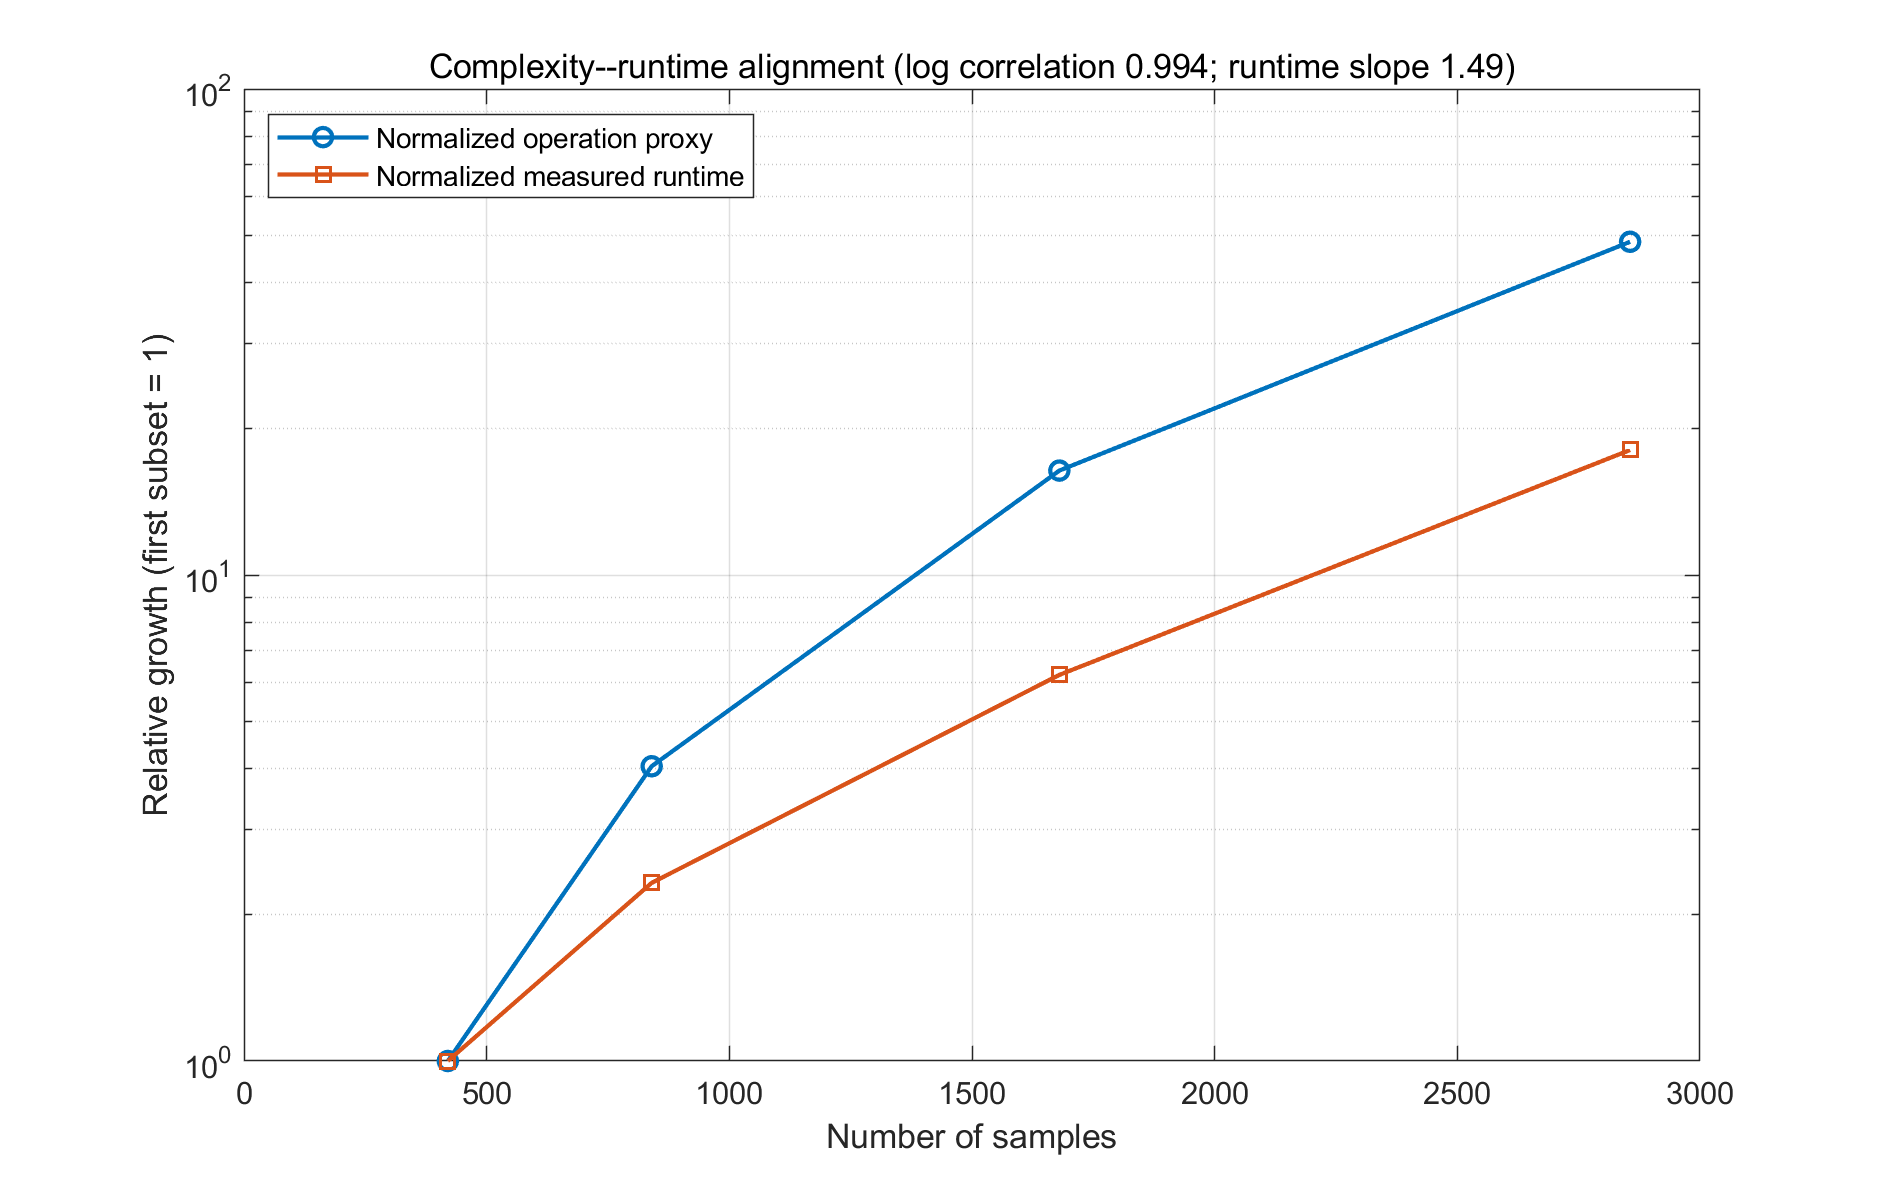
\includegraphics[width=0.78\textwidth]{complexity_runtime_alignment.png}
\caption{Alignment between measured MCS-NMF runtime and the normalized operation-count proxy on nested PIE subsets. Both axes use logarithmic scaling.}
\label{fig:complexityruntime}
\end{figure}

\begin{table}[!htbp]
\centering
\caption{End-to-end runtime under the unified MATLAB protocol (mean $\pm$ standard deviation over five paired runs, seconds).}
\label{tab:runtime}
\scriptsize
\resizebox{\textwidth}{!}{%
\begin{tabular}{lrrrrrrrr}
\toprule
Method & AR & PIE & MSRA25 & YaleB & COIL20 & COIL100 & MNIST & Optdigits \\
\midrule
MCS-NMF & 29.44 $\pm$ 0.46 & 25.92 $\pm$ 0.11 & 2.33 $\pm$ 0.37 & 14.07 $\pm$ 0.84 & 7.07 $\pm$ 0.22 & 78.45 $\pm$ 5.10 & 23.86 $\pm$ 4.15 & 5.66 $\pm$ 0.08 \\
HLPNMF & 7.48 $\pm$ 1.09 & 13.68 $\pm$ 2.22 & 2.15 $\pm$ 0.47 & 9.27 $\pm$ 0.12 & 3.45 $\pm$ 0.06 & 107.45 $\pm$ 3.58 & 52.69 $\pm$ 8.30 & 30.46 $\pm$ 4.18 \\
LpCNMF & 8.41 $\pm$ 0.68 & 7.52 $\pm$ 1.20 & 0.68 $\pm$ 0.07 & 4.51 $\pm$ 0.32 & 2.06 $\pm$ 0.08 & 21.13 $\pm$ 0.29 & 9.96 $\pm$ 0.11 & 1.82 $\pm$ 0.12 \\
PNLPSCONMF & 11.47 $\pm$ 2.09 & 16.12 $\pm$ 3.09 & 2.55 $\pm$ 0.19 & 9.06 $\pm$ 1.98 & 2.96 $\pm$ 0.50 & 94.81 $\pm$ 5.76 & 55.40 $\pm$ 6.54 & 25.56 $\pm$ 0.47 \\
SPNMF & 21.53 $\pm$ 2.21 & 33.45 $\pm$ 1.87 & 10.06 $\pm$ 0.30 & 22.70 $\pm$ 0.17 & 8.54 $\pm$ 0.24 & 247.96 $\pm$ 28.15 & 154.56 $\pm$ 4.87 & 103.65 $\pm$ 7.00 \\
CSDCP & 43.77 $\pm$ 8.44 & 46.01 $\pm$ 8.40 & 11.84 $\pm$ 2.32 & 36.81 $\pm$ 6.72 & 16.88 $\pm$ 0.10 & 232.21 $\pm$ 24.54 & 186.12 $\pm$ 21.61 & 81.66 $\pm$ 2.59 \\
LP & 0.44 $\pm$ 0.27 & 0.58 $\pm$ 0.01 & 0.13 $\pm$ 0.00 & 0.44 $\pm$ 0.00 & 0.38 $\pm$ 0.50 & 3.88 $\pm$ 0.04 & 3.36 $\pm$ 0.04 & 1.24 $\pm$ 0.01 \\
GOCNMF & 1.22 $\pm$ 0.28 & 0.70 $\pm$ 0.18 & 0.05 $\pm$ 0.04 & 0.47 $\pm$ 0.13 & 0.19 $\pm$ 0.05 & 2.62 $\pm$ 1.02 & 0.94 $\pm$ 0.87 & 0.20 $\pm$ 0.35 \\
OCSNMF & 0.42 $\pm$ 0.04 & 0.63 $\pm$ 0.03 & 0.15 $\pm$ 0.01 & 0.45 $\pm$ 0.02 & 0.17 $\pm$ 0.01 & 4.14 $\pm$ 0.06 & 3.36 $\pm$ 0.03 & 1.25 $\pm$ 0.04 \\
\bottomrule
\end{tabular}}
\end{table}


\subsection{Representation visualization and convergence}

Figure~\ref{fig:tsne} compares t-SNE projections of the original features, HLPNMF coefficients, and MCS-NMF semantic coefficients using identical stratified samples within each dataset. Both factorization methods improve class organization relative to the original space. MCS-NMF produces compact semantic groups on COIL20 and MSRA25 and organizes the overlapping YaleB representation into clearer local groups.

\begin{figure}[!htbp]
\centering
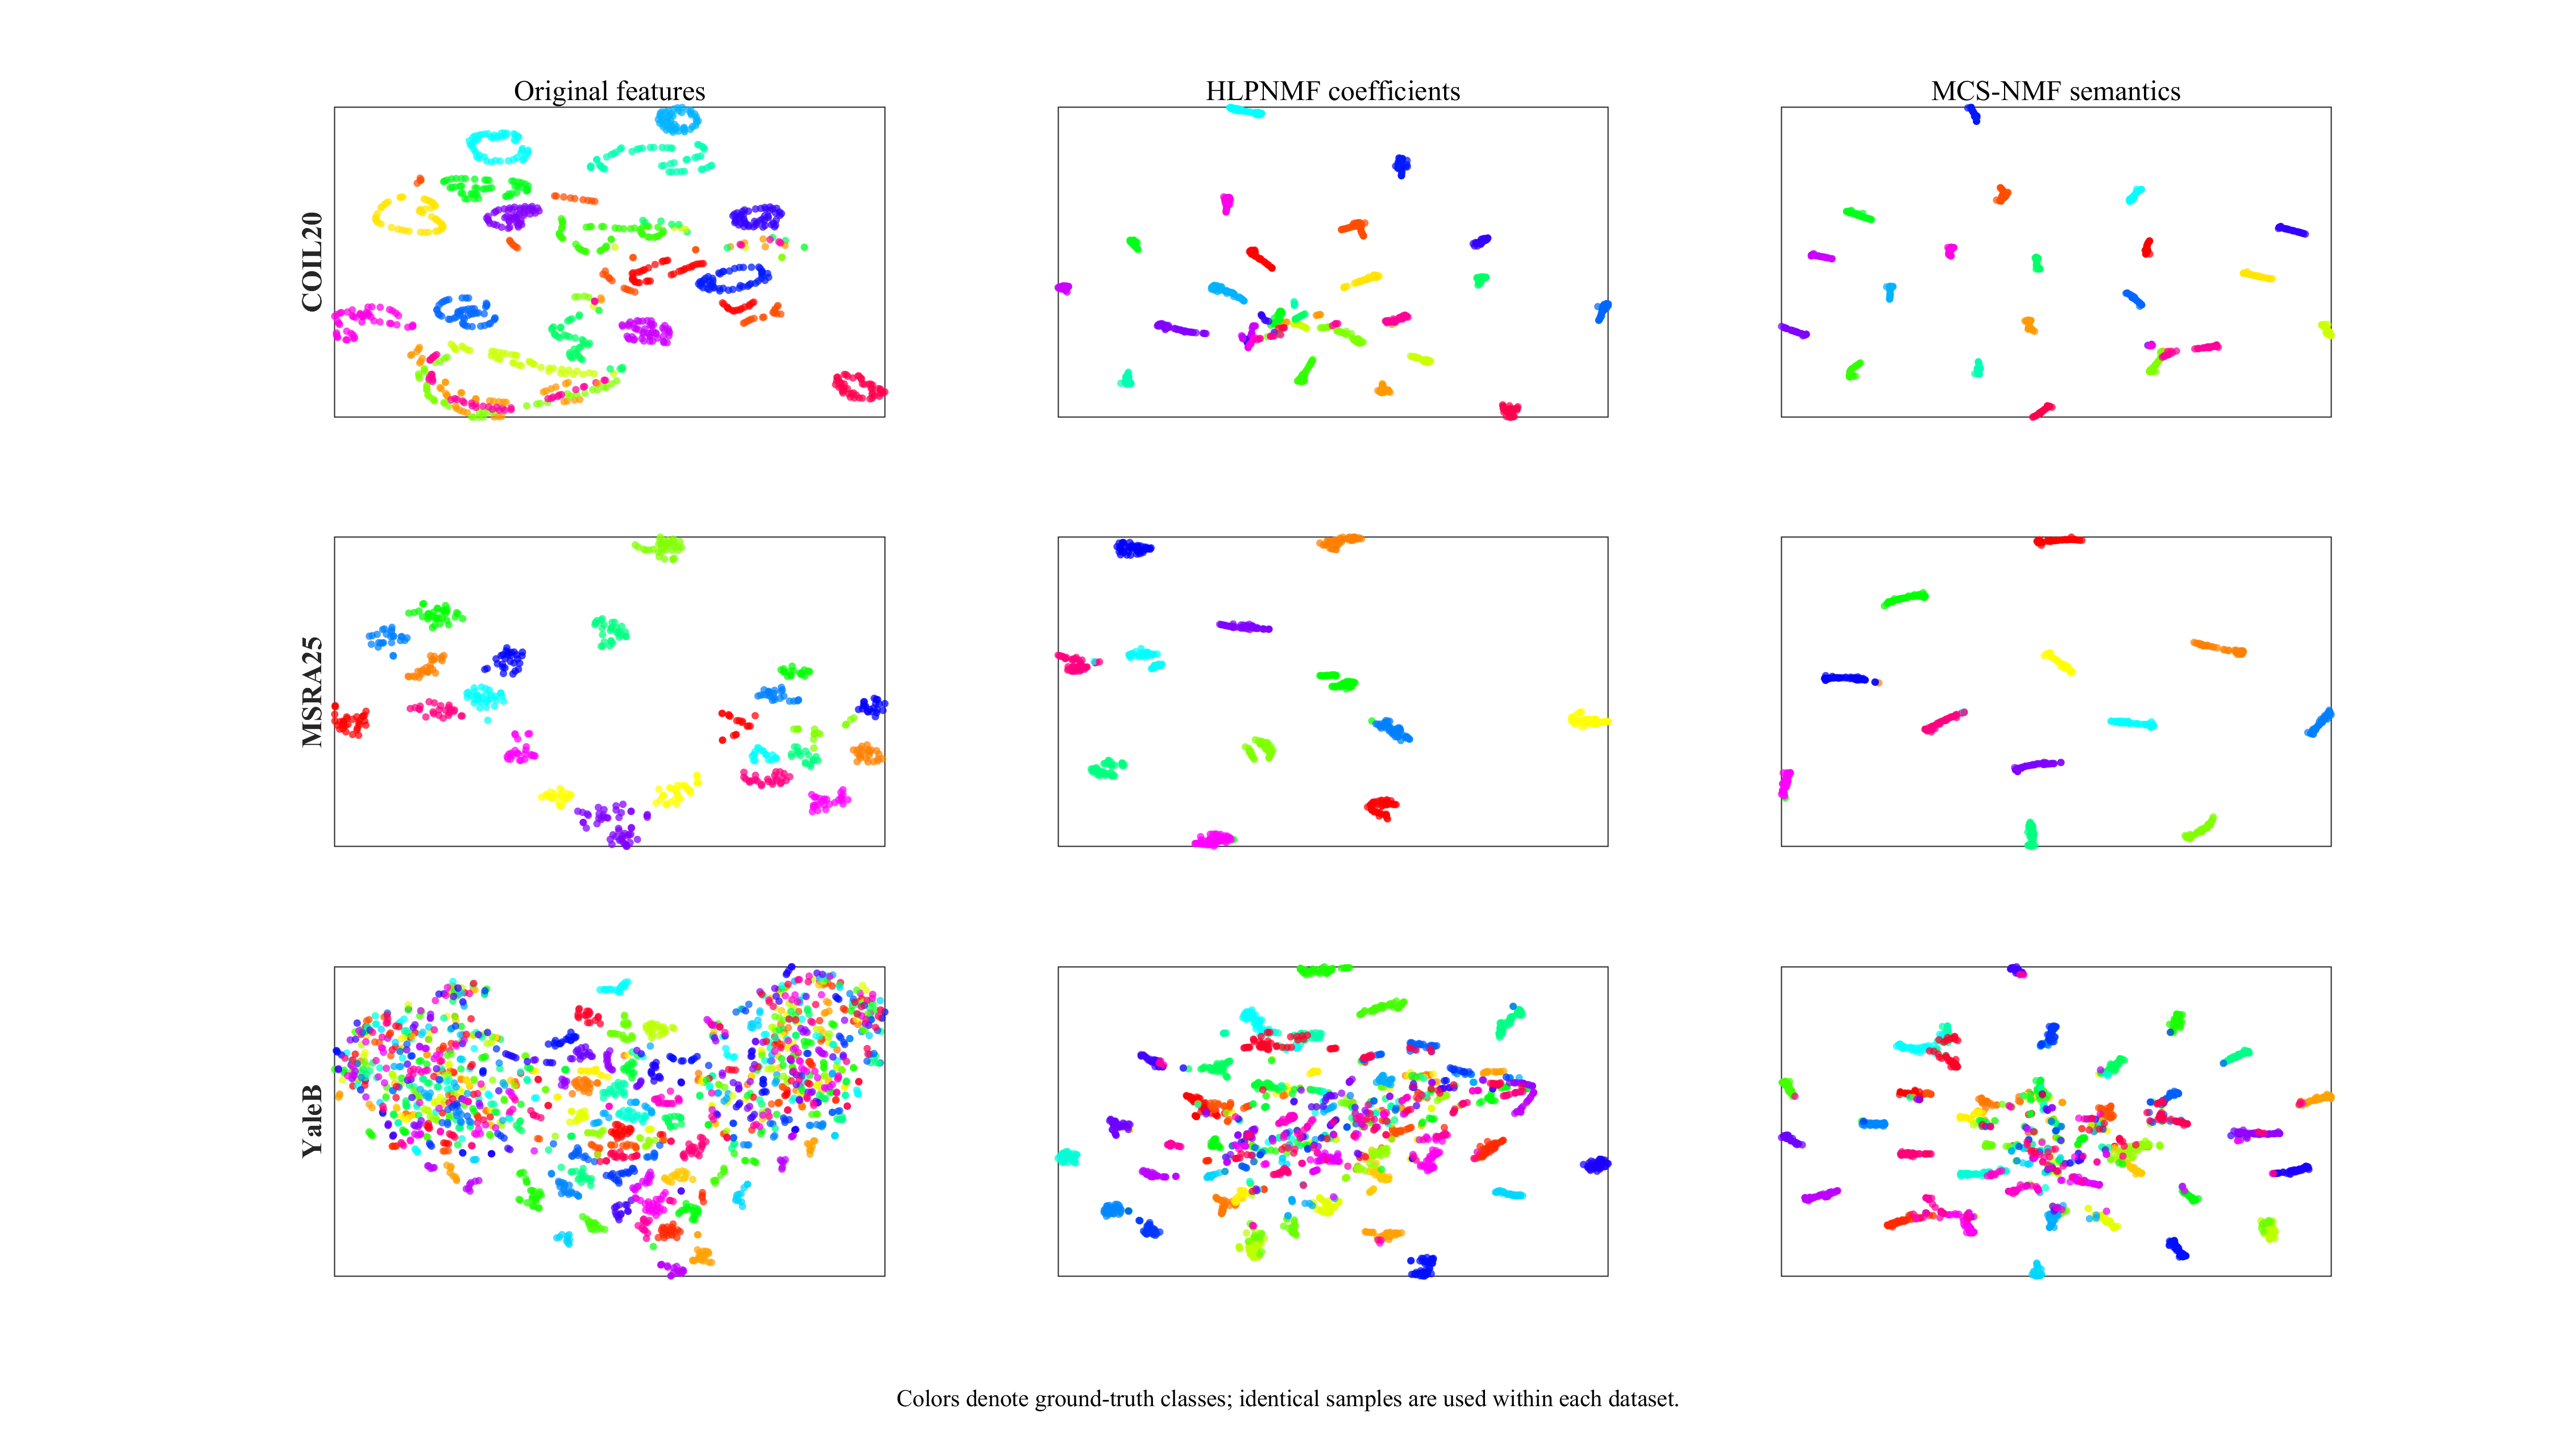
\includegraphics[width=0.98\textwidth]{tsne.png}
\caption{t-SNE projections of original features, HLPNMF coefficients, and MCS-NMF semantic coefficients. Colors denote ground-truth classes; identical samples and color maps are used within each dataset.}
\label{fig:tsne}
\end{figure}

The objective trajectories in Fig.~\ref{fig:convergence} decrease rapidly and then stabilize. Across the audited core runs, all factors and objective values were finite, the maximum final row-marginal error was below $9.65\times10^{-11}$, and the maximum column-marginal error was below $7.05\times10^{-12}$.

\begin{figure}[H]
\centering
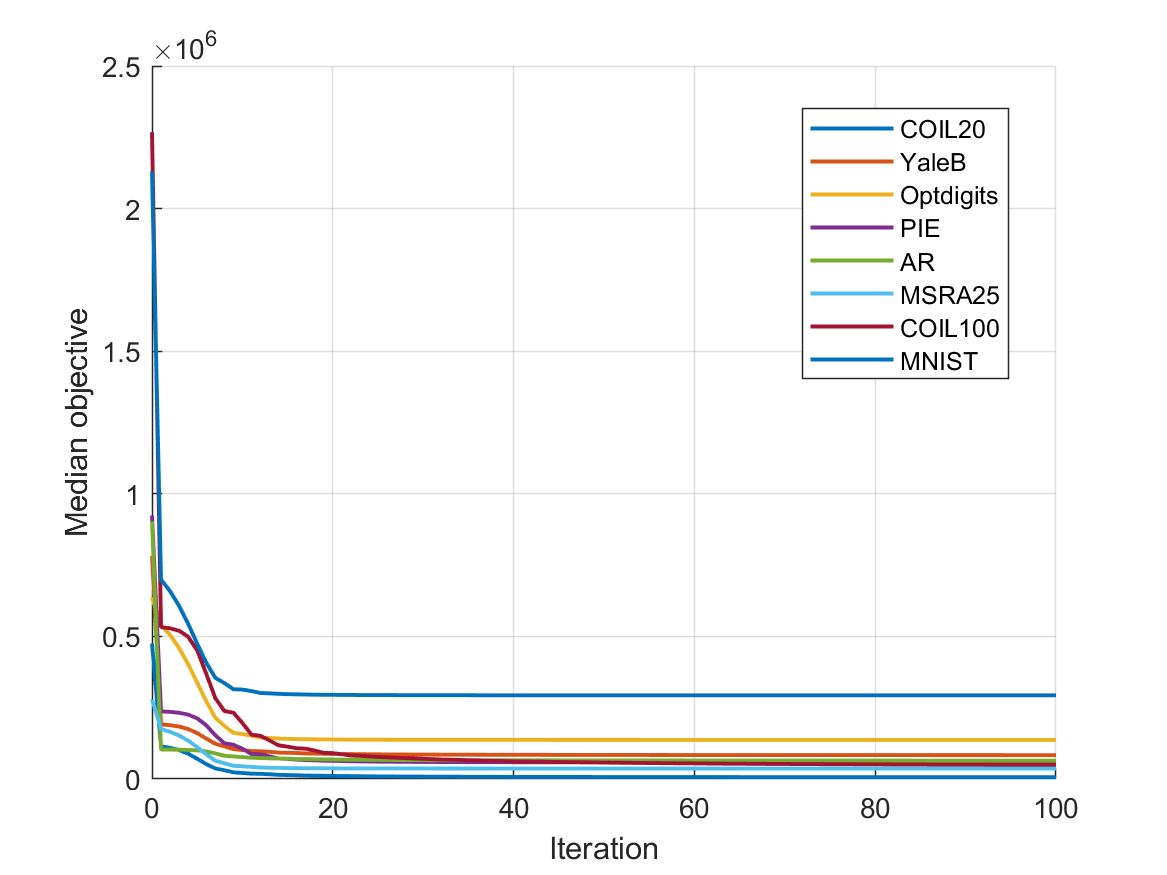
\includegraphics[width=0.86\linewidth]{convergence.png}
\caption{Median MCS-NMF objective value over alternating cycles.}
\label{fig:convergence}
\end{figure}
\FloatBarrier

\section{Discussion}

The experiments identify two roles of the transport constraint. First, it prevents unrestricted drift of aggregate class evidence during diffusion. Second, it acts as a global regularizer coupled to reconstruction. Its effect therefore depends on the labeled marginal and the dataset geometry. The empirical labeled prior is parameter free and effective across the main benchmarks, while the row-only ablation and prior-shift audit show that it is not equivalent to knowing the true unlabeled class proportions.

On AR, ERDNMF achieves the highest ACC and MCS-NMF achieves the highest NMI. On Optdigits, the paired NMI interval for MCS-NMF versus HLPNMF crosses zero. These results assign the leading method separately by dataset and metric. The solver preserves feasibility and monotone objective values, with numerical projection and relative-objective change defining its stopping behavior.

\section{Conclusion}

We presented MCS-NMF, a semi-supervised factorization model that places the unlabeled semantic coefficients in a labeled-prior transport polytope. The model combines reconstruction, high-order diffusion, row-simplex semantics, and aggregate class-mass conservation without adding a new regularization coefficient. An alternating multiplicative and exponentiated-gradient solver preserves feasibility and converges in objective value. Paired experiments on nine datasets and 12 baselines establish the performance gains and quantify the metric-specific outcomes on AR and Optdigits. Parameter, robustness, ablation, class-mass, long-tail, convergence, scalability, and t-SNE results characterize the global semantic constraint.

\section*{Data and code availability}
The benchmark data follow the public HLPNMF experimental collection, with Optdigits obtained from the standard UCI version. The implementation, fixed supervision masks, per-run outputs, and scripts used to generate the tables and figures are available at \url{https://github.com/matrix-research-lab-Wf/ScaleSem-NMF}.

\section*{Declaration of competing interest}
The authors declare no competing interests.

\section*{Declaration of generative AI use}
During the preparation of this work, the authors used a generative AI tool to improve the language and readability of the manuscript. The authors reviewed and edited the resulting text and take full responsibility for the content of the article.

\begin{thebibliography}{99}
\bibitem{Jain1999Clustering} A. K. Jain, M. N. Murty, P. J. Flynn, Data clustering: A review, ACM Computing Surveys 31(3) (1999) 264--323.
\bibitem{Jain2010Clustering} A. K. Jain, Data clustering: 50 years beyond K-means, Pattern Recognition Letters 31(8) (2010) 651--666.
\bibitem{Bair2013SSC} E. Bair, Semi-supervised clustering methods, WIREs Computational Statistics 5(5) (2013) 349--361.
\bibitem{VanEngelen2020Survey} J. E. van Engelen, H. H. Hoos, A survey on semi-supervised learning, Machine Learning 109(2) (2020) 373--440.
\bibitem{Lee1999NMF} D. D. Lee, H. S. Seung, Learning the parts of objects by non-negative matrix factorization, Nature 401 (1999) 788--791.
\bibitem{Lee2001Algorithms} D. D. Lee, H. S. Seung, Algorithms for non-negative matrix factorization, Advances in Neural Information Processing Systems 13 (2001) 556--562.
\bibitem{Gillis2014WhyHow} N. Gillis, The why and how of nonnegative matrix factorization, in: Regularization, Optimization, Kernels, and Support Vector Machines, Chapman and Hall/CRC, 2014, pp. 275--310.
\bibitem{Liu2012CNMF} H. Liu, Z. Wu, X. Li, D. Cai, T. S. Huang, Constrained nonnegative matrix factorization for image representation, IEEE TPAMI 34(7) (2012) 1299--1311.
\bibitem{Cai2011GNMF} D. Cai, X. He, J. Han, T. S. Huang, Graph regularized nonnegative matrix factorization for data representation, IEEE TPAMI 33(8) (2011) 1548--1560.
\bibitem{Zeng2014HypergraphNMF} K. Zeng, J. Yu, C. Li, J. You, T. Jin, Image clustering by hypergraph regularized non-negative matrix factorization, Neurocomputing 138 (2014) 209--217.
\bibitem{Yi2015LpSNMF} Y. Yi, Y. Shi, H. Zhang, J. Wang, J. Kong, Label propagation based semi-supervised non-negative matrix factorization for feature extraction, Neurocomputing 149 (2015) 1021--1037.
\bibitem{Lan2022LPNMF} L. Lan, T. Liu, X. Zhang, C. Xu, Z. Luo, Label propagated nonnegative matrix factorization for clustering, IEEE TKDE 34(1) (2022) 340--351.
\bibitem{Wang2015ConstraintNMF} D. Wang, X. Gao, X. Wang, Semi-supervised nonnegative matrix factorization via constraint propagation, IEEE Transactions on Cybernetics 46(1) (2016) 233--244.
\bibitem{Wang2022PNLP} C. Wang, J. Zhang, T. Wu, M. Zhang, G. Shi, Semi-supervised NMF with positive and negative label propagations, Applied Intelligence 52(9) (2022) 9739--9750.
\bibitem{Yin2023HSSNMF} J. Yin, S. Peng, Z. Yang, B. Chen, Z. Lin, Hypergraph based semi-supervised symmetric NMF for image clustering, Pattern Recognition 137 (2023) 109274.
\bibitem{Mo2024PNLPSCNMF} Y. Mo, X. Li, J. Mei, Semi-supervised NMF with label propagation and constraint propagation, Engineering Applications of Artificial Intelligence 133 (2024) 108196.
\bibitem{Li2025GOCNMF} J. Li, C. Li, Graph regularized one-hot-constrained NMF for data representation, Engineering Applications of Artificial Intelligence 156 (2025) 111224.
\bibitem{Li2025OCSNMF} J. Li, C. Li, One-hot constrained symmetric NMF for image clustering, Pattern Recognition 162 (2025) 111427.
\bibitem{Yang2025SPNMF} X. Yang, T. Zhu, S. Peng, F. Nie, Z. Lin, Semi-supervised pivotal-aware NMF with label and pairwise constraint propagation, Pattern Recognition 157 (2025) 110933.
\bibitem{Li2026HLPNMF} J. Li, X. Zhou, X. Shen, C. Li, High-order label propagation-guided NMF for semi-supervised clustering, Pattern Recognition 180 (2026) 114657.
\bibitem{Yang2016Doubly} Z. Yang, J. Corander, E. Oja, Low-rank doubly stochastic matrix decomposition for cluster analysis, Journal of Machine Learning Research 17 (2016) 1--25.
\bibitem{Tai2021Sinkhorn} K. S. Tai, P. Bailis, G. Valiant, Sinkhorn label allocation: Semi-supervised classification via annealed self-training, in: ICML, 2021, pp. 10065--10075.
\bibitem{Wang2026BSNMF} J. Wang, B. Yao, Y. Ma, G. Wu, R. Zhao, F. Nie, Balanced symmetric non-negative matrix factorization, Neurocomputing 695 (2026) 134013.
\bibitem{Li2022SinkhornNMF} S. Li, W. Li, P. Gan, L. Jiang, Multi-constrained non-negative matrix factorization algorithm based on Sinkhorn distance feature scaling, Journal of Electronics \& Information Technology 44(12) (2022) 4384--4394.
\bibitem{Xing2021DSSNMF} Z. Xing, M. Wen, J. Peng, J. Feng, Discriminative semi-supervised NMF for data clustering, Engineering Applications of Artificial Intelligence 103 (2021) 104289.
\bibitem{Li2025EDNMF} J. Li, X. Shen, C. Li, Y. Li, Elements discriminative NMF for data clustering, Engineering Applications of Artificial Intelligence 156 (2025) 111210.
\bibitem{Xing2021GNMFLD} Z. Xing, Y. Ma, X. Yang, F. Nie, Graph regularized NMF with label discrimination for data clustering, Neurocomputing 440 (2021) 297--309.
\bibitem{Peng2021CSNMF} S. Peng, W. Ser, B. Chen, Z. Lin, Robust semi-supervised NMF for image clustering, Pattern Recognition 111 (2021) 107683.
\bibitem{Chavoshinejad2023S4NMF} J. Chavoshinejad, S. A. Seyedi, F. Akhlaghian Tab, N. Salahian, Self-supervised semi-supervised NMF for data clustering, Pattern Recognition 137 (2023) 109282.
\bibitem{Zhu2003GaussianFields} X. Zhu, Z. Ghahramani, J. Lafferty, Semi-supervised learning using Gaussian fields and harmonic functions, in: ICML, 2003, pp. 912--919.
\bibitem{Zhou2004LGC} D. Zhou, O. Bousquet, T. N. Lal, J. Weston, B. Sch"olkopf, Learning with local and global consistency, Advances in Neural Information Processing Systems 16 (2004).
\bibitem{Jing2026SNMFWLP} W. Jing, L. Lu, W. Ou, Semi-supervised NMF with weighted label propagation for data representation, Signal Processing 241 (2026) 110407.
\bibitem{Qiao2018GraphReview} L. Qiao, L. Zhang, S. Chen, D. Shen, Data-driven graph construction and graph learning: A review, Neurocomputing 312 (2018) 336--351.
\bibitem{Gao2022HypergraphReview} Y. Gao, Z. Zhang, H. Lin, X. Zhao, S. Du, C. Zou, Hypergraph learning: Methods and practices, IEEE TPAMI 44(5) (2022) 2548--2566.
\bibitem{Song2023GSSLReview} Z. Song, X. Yang, Z. Xu, I. King, Graph-based semi-supervised learning: A comprehensive review, IEEE TNNLS 34(11) (2023) 8174--8194.
\bibitem{Kuhn1955Hungarian} H. W. Kuhn, The Hungarian method for the assignment problem, Naval Research Logistics Quarterly 2 (1955) 83--97.
\bibitem{Vinh2010NMI} N. X. Vinh, J. Epps, J. Bailey, Information theoretic measures for clusterings comparison, Journal of Machine Learning Research 11 (2010) 2837--2854.
\end{thebibliography}

\end{document}
